\documentclass[a4paper,oneside,12pt]{report}

\usepackage{../custom}

\newcommand{\barg}{\si{\bar}\text{g}} 

\usepackage{fancyhdr} 
\fancyhf{}
\fancyhead[R]{P3 – 2014 - gr25 }   
\fancyfoot[C]{\thepage}                     
\renewcommand\headrulewidth{0pt}
\pagestyle{fancy}
\newcommand{\barg}{\si{\bar}\text{g}} 
\usepackage[backend=biber]{biblatex}
\addbibresource{../biblio.bib}

\begin{document}

\begin{titlepage}
    \begin{center}
        \vspace*{1cm}
        
        \Huge
	\textbf{Procédé de production d'ammoniac}
        
        \vspace{1cm}
        
        \textbf{Groupe 1225}
        
        \vspace{0.5cm}
        
        \large
        Un rapport réalisé dans le cadre du cours\\
        
        \LARGE
        Projet Q3 - LFSAB1503
        \vspace{0,5cm}
        
        %\includegraphics[scale = 0.25]{img/divers/coverpicture.png}        
        %\vfill
        
        %\includegraphics[scale = 0.2]{img/divers/epl-logo.jpg}
        %\vspace{1cm}

        \vfill 
        \large
        
	de Bellefroid Cédric ($32631100$) \\
	Dénos Cyril ($62811300$) \\
        de Wasseige John ($52241300$) \\
	Dispas David ($71891200$) \\
	Libeer Cassian  ($65161200$) \\
        Malengreau Tim ($66081300$) \\
	Paquet Arnaud ($36681300$) \\       
        
    \end{center}
\end{titlepage}


\tableofcontents

\chapter{T\^ache 1}
<<<<<<< HEAD
\documentclass[a4paper, oneside, 12pt]{article}

\usepackage{../custom}

\usepackage[backend=biber]{biblatex}
\addbibresource{biblio.bib}

\title{Rapport 2}
\author{Groupe 1225}
\date{\today}

\begin{document}

\maketitle

\section{Introduction}

Ce second rapport est une extension et une amélioration du rapport rendu 
en S2 et a pour but d'étudier plus en détail la production d'ammoniac. 
Il comprend un flow sheet qui permet de voir les flux de matières en 
les différentes étapes de la synthèse par le procédé Haber-Bosh. 
Il comprend aussi un calcul détaillé des aspects énergétiques dans le réformateur primaire.
S’y trouve ensuite une explication du fonctionnement de l’outil de calcul
réalisé sur \textsc{matlab} (ainsi que l'outis de calcul en annexe).
Celui-ci permet le calcul des flux entrants et sortants en fonction 
de la quantité d'ammoniac voulue dans la journée ainsi que de la 
température dans le réformateur primaire. Il calcul également les aspects énergétiques 
lors des différentes étapes. 
Et enfin ce rapport se termine par une analyse de l'effet du changement 
des variables que sont la température et la quantité d'ammoniac produite 
sur le bilan de matière.

\section{Bilan de matière}
\label{sec:bilan_matiere}

Une partie de la t\^ache 1 consiste à réaliser un outil de gestion
pour pouvoir déterminer les quantités de matières première nécessaires,
lorsque 2 paramètres varient. 
Les paramètres sont la température à la sortie de réacteur primaire ainsi
que la quantité d'ammoniac produite par jour. 
On les notera respectivement $T$ et $m_{\ce{NH3}}$.

À travers cette section, nous décrirons différentes réactions et nous 
supposons que le lecteur sait quelle réaction a lieu à quel moment ainsi 
que l'ordre des réactions durant tout le processus.
Un flow-sheet simplifié de l'ensemble du processus détaillant chacune
des réactions se trouve à la section \ref{sec:flowsheet}.

\subsection{Quantité d'air}

Nous connaissons la masse d'ammoniac à produire par jour, 
et par conséquent son nombre de moles ($n_{\ce{NH3}} = m_{\ce{NH3}}/M_{\ce{NH3}}$).
Les nombres de moles seront généralement écrits en fonction de $m_{\ce{NH3}}$ 
de façon à montrer la relation par rapport au paramètre qui varie.

À partir de la réaction suivante,

\begin{equation*}
	\ce{\frac{3}{2} \, H2 + \frac{1}{2} \, N2 -> NH3} 
\end{equation*}

on détermine les quantités de \ce{H2} et de \ce{N2} nécessaires.

\begin{align}
	n_{\ce{H2}} = \frac{3}{34} \, m_{\ce{NH3}} 
	\label{eq:moles_H2} \\
	n_{\ce{N2}} = \frac{1}{34} \, m_{\ce{NH3}} \nonumber
\end{align}

Or la seule source d'azote est lorsque l'air entre dans le réacteur secondaire.
En connaissant les proportions de l'azote, de l'oxygène et de l'argon dans 
l'air, on peut facilement obtenir les quantités de \ce{O2} et de \ce{Ar}.

\begin{align*}
	n_{\text{air}} = \frac{1}{0.78} \, n_{\ce{N2}} = \frac{25}{663} \, m_{\ce{NH3}} \\
	n_{\ce{O2}} = 0.21 \, n_{\text{air}} = \frac{7}{884} \, m_{\ce{NH3}} \\
	n_{\ce{Ar}} = 0.01 \, n_{\text{air}} = \frac{1}{2652} \, m_{\ce{NH3}} 
\end{align*}

\subsection{Quantité de méthane et d'eau}

Il nous reste maintenant à déterminer les quantités de \ce{CH4} et de \ce{H2O}.
On voit que la seule réaction nécessitant de l'oxygène est celle du 
réformage secondaire. Ceci nous permet de conna\^itre toutes les quantités 
associées à cette réaction. 
Afin de ne pas oublier à quelle réaction est associée chaque quantité, 
on notera \textit{rp} (resp. \textit{rs}) pour réformage primaire (resp. secondaire)
et \textit{wgs} pour Water-Gas-Shift.

\begin{equation*}
	\ce{2CH4 + O2 -> 2CO + 4H2}
\end{equation*}

Dès lors, 

\begin{align}
	n_{\ce{CO}, rs} = n_{\ce{CH4}, rs} 
	= 2 \, n_{\ce{O2}} = \frac{7}{442} \, m_{\ce{NH3}} 
	\label{eq:moles1_ref_sec} \\
	n_{\ce{H2}, rs} = 4 \, n_{\ce{O2}} = \frac{7}{221} \, m_{\ce{NH3}}
	\label{eq:moles2_ref_sec}
\end{align}

Interessons nous maintenant au réformage primaire.
\begin{align*}
	&\ce{CH4 + H2O <-> CO + 3H2} \\
	&\ce{CO + H2O <-> CO2 + H2}
\end{align*}

Comme les deux réactions sont à l'équilibre,
il va falloir déterminer leurs constantes d'équilibres sans
oublier qu'elles s'influencent mutuellement.
C'est ici qu'intervient le paramètre $T$. On va donc commencer
par calculer les $\Delta_r G^{\circ}$ afin de conna\^itre les constantes
d'équilibres $K(T)$, pour finalement déterminer les quantités des différents composés
à l'équilibre.

\paragraph{Calcul des constantes d'équilibres $K(T)$}

On a déjà vu précedement que les valeurs des capacités calorifiques
à pression constante varient avec la température. Afin d'avoir un outil de gestion
le plus précis possible, nous allons utiliser les équations de Shomate pour calculer 
les enthalpies et entropies standards. 
Lors du précédent rapport, nous avions décris que $C_{p,m}^{\circ} = A + B \, T + C \, T^2$,
on ajoute un degré de précision en posant

\begin{equation}
	C_{p,m}^{\circ} = A + B \, t + C \, t^2 + D \, t^3 + \frac{E}{t^2}
	\quad \text{avec} \quad t = \frac{T[K]}{1000}
	\label{eq:shomate}
\end{equation}

les valeurs des différents coefficients\footnote{Il faut ajouter deux autres 
coefficients F et G à cause des constantes d'intégrations pour les
enthalpies et entropies.} se trouvent \cite{shomate} dans \texttt{getCoefficients}.
On en déduit donc les valeurs des enthalpies et entropies
à partir de l'équation \ref{eq:shomate} dans \texttt{getDeltaH\_and\_S}  

\begin{align*}
	\Delta_f H_{T2}^{\circ} &= \Delta_f H_{T1}^{\circ} 
	+ \int_{T1}^{T2} C_{p,m} \, \dif{T} \\ 
				 &= \Delta_f H_{T1}^{\circ} 
	+ A \, t + B \, \frac{t^2}{2}  + C \,  \frac{t^3}{3} 
	+ D \, \frac{t^4}{4} - \frac{E}{t} + K_{1} \\		 
	S_{T2}^{\circ}  &= S_{T1}^{\circ} + \int_{T1}^{T2} 
	\frac{C_{p,m}}{T} \, \dif{T} \\
			&= S_{T1}^{\circ} + A \, \ln{t} 
	+ B \, t + C \, \frac{t^2}{2} 
	+ D \, \frac{t^3}{3} - \frac{E}{2 t^{2}} + K_{2} 
\end{align*}

Afin de ne pas trop alourdir ce document, les détails des calculs sont ignorés. 

On détermine ensuite l'enthalpie libre de Gibbs via la relation 

\begin{equation*}
	\Delta_r G^{\circ} = \Delta_r H^{\circ} 
	- T \, \Delta_r S^{\circ}
\end{equation*}

et finalement la constante d'équilibre 

\[ 
K(T) = \exp{\left(\frac{- \Delta_r G}{R \, T}\right)} 
\]

Les constantes d'équilibre des deux réactions du réformage primaire 
sont calculées dans \texttt{getEqConstantsRef}.

\paragraph{Calcul des pressions partielles à l'équilibre}

Les tableaux \ref{tab:reaction1_primaire} et \ref{tab:reaction2_primaire} nous 
permettent de conna\^itre les quantités des réactifs et des produits à l'équilibre. 

\begin{table}
	\centering
	\begin{tabular}{l|c|c|c|c|c}
		 & $\ce{CH4}$ & $\ce{H2O}$ & $\ce{CO}$ & $\ce{3H2}$ & $n_{gaz}$ \\
		\hline
		$p_{i}$ & $n_{\ce{CH4}}$ & $n_{\ce{H2O}}$ & $0$ & $0$ &
		$n_{\ce{CH4}} + n_{\ce{H2O}}$ \\
		$p_{eq}$ & $n_{\ce{CH4}} - \xi_1$ & $n_{\ce{H2O}} - \xi_1$ & 
		$\xi_1$ & $3 \, \xi_1$ & $n_{\ce{CH4}} + n_{\ce{H2O}} + 2 \, \xi_1 $\\
	\end{tabular}
	\caption{Première réaction du réformage primaire à l'équilibre}
	\label{tab:reaction1_primaire}
\end{table}

\begin{table}
	\centering
	\begin{tabular}{l|c|c|c|c|c}
		 & $\ce{CO}$ & $\ce{H2O}$ & $\ce{CO2}$ & $\ce{H2}$ & $n_{gaz}$ \\
		\hline
		$p_{i}$ & $\xi_1$ & $n_{\ce{H2O}} - \xi_1$ & $0$ & $3 \, \xi_1$ &
		$n_{\ce{H2O}} + 3 \, \xi_1$ \\
		$p_{eq}$ & $\xi_1 - \xi_2$ & $n_{\ce{H2O}} - \xi_1 - \xi_2$ & 
		$\xi_2$ & $3 \, \xi_1 + \xi_2$ & $n_{\ce{H2O}} + 3 \, \xi_1 $\\
	\end{tabular}
	\caption{Deuxième réaction du réformage primaire à l'équilibre}
	\label{tab:reaction2_primaire}
\end{table}

Il s'agit maintenant de résoudre 4 équations afin de déterminer nos inconnues que 
sont $\xi_1$, $\xi_2$, $n_{\ce{CH4}}$ et $n_{\ce{H2O}}$. 
On a tout d'abord les deux liées aux activités et constantes $K$, que nous déduisons
à partir des informations des réactions à l'équilibre.

\begin{align}
	K_1 &= \frac{p_{tot}^2 \, (\xi_1 - \xi_2) \, (3 \xi_1 + \xi_2)^3}
	{p_{0}^2 \, (n_{\ce{CH4}} + n_{\ce{H2O}} + 2 \xi_2)^2 \, (n_{\ce{CH4}} - 
	\xi_1) \, (n_{\ce{H2O}} - \xi_1 - \xi_2 )} 
	\label{eq:systeme1} \\
	K_2 &= \frac{\xi_2 \, (3 \xi_1 + \xi_2)}
	{(\xi_1 - \xi_2) \, (n_{\ce{H2O}} - \xi_1 - \xi_2)}
	\label{eq:systeme2}
\end{align}

Les deux suivantes s'appuyent sur le fait que si une mole d'un composé $X$ est
produite à une réaction $\alpha$, une mole de ce même composé sera disponible 
dans la réaction suivante.

On a pu voir dans le tableau \ref{tab:reaction1_primaire} qu'il reste après 
équilibre exactement $n_{\ce{CH4}} - \xi_1$ moles de \ce{CH4}, qui seront 
entièrement consommées pendant le réformage secondaire. 
Par l'équation \ref{eq:moles1_ref_sec}, on a que 

\begin{equation}
	n_{\ce{CH4}} - \xi_1 = \frac{7}{442} \, m_{\ce{NH3}}
	\label{eq:systeme3}
\end{equation}

Pour finir, on remarque que 

\begin{equation*}
	n_{\ce{H2}} = n_{\ce{H2}, rp} + n_{\ce{H2}, rs} + n_{\ce{H2}, wgs}
\end{equation*}

on vient de voir (tableau \ref{tab:reaction2_primaire})
que $n_{\ce{H2}, rp} = 3 \, \xi_1 + \xi_2$, nous connaissons égalemment
$n_{\ce{H2}}$ (équation \ref{eq:moles_H2})
et $n_{\ce{H2}, rs}$ (équation \ref{eq:moles2_ref_sec}), on a ensuite 

\begin{align*}
	n_{\ce{H2}, wgs} = n_{\ce{CO}, \text{total}} 
	&= n_{\ce{CO}, rp} + n_{\ce{CO}, rs} \quad &\text{(voir flow-sheet)} \\
	&= \xi_1 - \xi_2 + \frac{7}{442} \, m_{\ce{NH3}} 
	\quad &\text{(voir tableau \ref{tab:reaction2_primaire} et eq \ref{eq:moles1_ref_sec})}
\end{align*}

Ce qui nous donne 

\begin{equation}
	4 \, \xi_1 = \frac{9}{221} \, m_\ce{NH3}
	\label{eq:systeme4}
\end{equation}

Nous résolvons le système de 4 équations 
(\ref{eq:systeme1}, \ref{eq:systeme2}, \ref{eq:systeme3}, \ref{eq:systeme4})
dans \texttt{solveG}.

\section{Fonctionnement de l'outil de calcul}

L'outil de calcul a été réalisé en matlab et prends en considération 
deux variables : la température du réacteur primaire (en K) et la quantité 
d'ammoniac (en tonnes) que l'on souhaite produire en 24h. 

Nous commençons tout d'abord par calculer les enthalpies (incl. Gibbs) 
et entropies des réactions du réacteur primaire (vaporeformage).
Nous calculons ensuite les constantes d'équilibres pour les deux réactions. 
Avec les hypothèses posées sur les réactions (toutes sont complètes 
exceptées celles s'effectuant dans le réacteur primaire),
et avec la masse désirée de \ce{NH3}, nous calculons les masses 
nécessaires de \ce{H2}, \ce{N2}. Puisque l'azote est fourni
par l'air, nous déterminons la masse de \ce{O2} fournie (ainsi que la masse de \ce{Ar}, 
mais l'argon est un gaz noble et n'intervient pas dans la réaction). 

Avec les hypothèses et la masse de \ce{O2}, nous déterminons la quantité de \ce{CH4} 
utilisé dans le réacteur secondaire et donc la production de \ce{H2} dans ce réacteur. 
Nous savons désormais déterminer la quantité de \ce{H2} à produire dans 
le réacteur primaire, et grâce à la constante d'équilibre déterminée plus tôt, 
nous pouvons déterminer la quantité de \ce{CH4} nécessaire pour les deux réactions.
L'outil nous permet également de calculer la quantité minimum de \ce{H2O} à fournir
pour que toutes les équations se passent comme prévu. 

Il est à noter que l'outil nous fourni des valeurs en tonnes par jour.

\section{Tubes}

Nous recherchons le nombre de tubes nécaissaire à l'acheminement du 
méthane et de l'eau dans le reformateur primaire.

Soit $x$ le nombre de tubes, nous avons l'équation suivante :
\[
	\dot{V} = A \, \dot{c} \, x
\]

Avec $\dot{V}$ le débit, $A$ la section d'un tuyau 
et $\dot{c}$ la vitesse superficielle à l'entrée du réacteur.
Le volume peut être calculé grace à la loi des gaz parfaits,
on considère donc que \ce{H2O} se comporte comme un gaz parfait,
pour plus de précision on pourra éventuellement utiliser l'équation
d'état de van der Waals.
\[
	V = \frac{n R T}{p}
\]

Si l'on considère notre calcul en un temps d'une seconde, 
la simplification des deux formules ci-dessus nous amène à
\[
	x = \frac{n R T}{A \dot{c} \, p}
\]

Or nous savons que la vitesse superficielle à l'entrée des tubes 
vaut $2 \si{\meter\per\second}$,
que leurs diamètre est de $1 \si{\centi\meter}$ 
(la section d'un tube est $A = \pi r^2$),
et qu'il y a une pression de $31 \si{\bar}$ à l'entrée.
Les seules inconnues sont donc la température et les nombres de moles
de produit entrant, c'est-à-dire de \ce{CH4} et de \ce{H2O},
que nous avons déterminé dans la section \ref{sec:bilan_matiere}.

Prenons l'exemple, pour une quantité d'ammoniac de $1500 \si{\tonne}$.

\begin{align*}
	n_{CH_{4}} = 7,56 \si{\kilo\per\second} / 0,016 \si{\kilo\per\mole} 
	= 472,18 \si{\mole\per\second} \\
	n_{H_{2}O} = 18,94 \si{\kilo\per\second}/ 0,016 \si{\kilo\per\mole}
	= 1052,22 \si{\mole\per\second}
\end{align*}

Grâce aux autres valeurs données dans l'énoncé 
nous pouvons calculer le nombre de tubes nécessaire 

\[
	x = \frac{(n_{CH_{4}}+n_{H_{2}O}) \cdot 8,314 \cdot1080}
	{\pi(0,05^2) \cdot 2 \cdot (31.10^5)} = 281,1
\]

Il faut donc 282 tuyaux pour assurer l'approvionnnement 
des composés dans le reformateur primaire.

La fonction \texttt{getTubesNumber} donne le
nombre de tubes requis en fonction des paramètres de départ (la masse d'ammoniac 
à produire et la température du réformeur primaire).

\section{Bilan énergétique de la partie réformeur primaire-four}

La première réaction - le craquage du méthane - qui se produit dans le réformeur primaire,
est une réaction endothermique. Nous devons donc lui fournir de l'énergie sous 
forme de chaleur, ce r\^ole va être rempli par le four. 
La réaction de combustion qui a lieu dans le four est la suivante

\[
	\ce{CH4 + 2O2 -> CO2 + 2H2O}
\]

Afin de connaître les quantités de méthane et d'oxygène qu'il faut
introduire dans le four, nous devons étudier les bilans énergétiques
des réactions ayant lieu dans ce réformateur. Les calculs exposés dans cette section 
sont fait pour une température dans le réformateur de $1080 \si{\kelvin}$
et pour une production journalière d'ammoniac de $1500 \si{\tonne}$. 
Bien sur ces résultats sont facilement transposables
à d'autres données à l'aide de notre outil de gestion.

Il faut tout d'abord calculer la chaleur nécessaire dans le réformeur primaire.
La différence d'enthalpie de réaction du craquage du méthane vaut $+225.7 \si{\kilo\joule}$
à $1000 \si{\kelvin}$, et celle de la deuxième réaction
vaut $-34.8 \si{\kilo\joule}$ à la même température.
La première est fortement endothermique tandis que la deuxième est exothermique.
Il faut fournir une quantité de chaleur $Q$ pour que la réaction endothermique
puisse avoir lieu, tout en tenant compte que le rendement énergétique de 
la réaction de combustion du four vaut $\eta = 0.75$.
Le nombre de moles qui vont réagir dans les réactions du réformeur primaire 
sont $\xi_1$ et $\xi_2$ (tableaux \ref{tab:reaction1_primaire} 
et \ref{tab:reaction2_primaire}).

On a donc que 
\[
	Q = n_{\ce{CH4},\text{four}} \cdot \Delta_r H_{\text{four}} \cdot \eta
\]

et 
\[
	-Q = \xi_1 \cdot \Delta_r H_{rp,1} + \xi_2 \cdot \Delta_r H_{rp,2}
\]

On obtient une équation à résoudre pour obtenir $n_{\ce{CH4},\text{four}}$, et on a ensuite
la quantité d'oxygène qu'il faut insérer $n_{\ce{O2},\text{four}} = 2 \cdot n_{\ce{CH4},\text{four}}$.

Ce bilan énergétique est modélisé dans \texttt{getHovenMasses}.

\section{Flow-sheet}
\label{sec:flowsheet}

La figure \ref{fig:flowsheet} présente un flow-sheet simplifié du processus 
de production d'ammoniac que nous étudions.

\begin{figure}[h!]
	\begin{center}
		\begin{tikzpicture}
[node distance = 7em]

\tikzstyle{output} = [diamond, draw, fill=blue!20, 
    text width=3em, text badly centered, node distance=3cm, inner sep=0pt]
\tikzstyle{block} = [rectangle, draw, fill=blue!20, 
    text width=15em, text centered, rounded corners, minimum height=4em]
\tikzstyle{line} = [draw, -latex']
\tikzstyle{input} = [draw, ellipse,fill=red!20, node distance=3cm,
    minimum height=2em]
    
\node [block] (primaire) {Reformage primaire (T)\\
	\ce{CH4 + H2O <=> CO + 3H2} \\
	\ce{CO + H2O <=> CO2 + H2}};
\node [input, left = 2em of primaire] (H2O) {\ce{H2O}};
\node [block, right = 2em of primaire] (four) {Four: Combustion \ce{CH4} ($\eta = 75\%$) 
($\simeq 1300K$)\\
	\ce{CH4 + 2O2 -> CO2 + 2H2O}};
\node [input, above = 3em of four] (O2) {\ce{O2}};
\node [input, above = 3em of primaire] (CH4) {\ce{CH4}};
\node [block, below of=primaire] (secondaire) {Reformage secondaire ($\simeq 1200K$)\\
	\ce{2CH4 + O2 -> 2CO + 4H2}};
\node [input, right = 1em of secondaire] (air) {Air ($21\% \ce{O2} 78\% \ce{N2} 
	1\% \ce{Ar}$)};
\node [block, below of=secondaire] (wgs) {Water-Gas-Shift ($\simeq 500-700K$)
	\ce{CO + H2O -> CO2 + H2}};
\node [block, below of=wgs] (abso) {Absorbtion du \ce{CO2} et compression};	
\node [output, right = 2em of abso] (CO22) {\ce{CO2}};	
\node [output, left = 2em of abso] (H2O2) {\ce{H2O}};
\node [block, below of=abso] (synthese) {Synthèse \ce{NH3} et séparation de l'argon \\
(Sortie réacteur: 270bar, 750K) \\
	\ce{3H2 + N2 <=> 2NH3}};
\node [output, below of=synthese] (NH3) {\ce{NH3}};
\node [output, right = 2em of synthese] (argon) {\ce{Ar}};


\path [line] (primaire) -- node[anchor = east] {\ce{H2} \ce{CH4} \ce{CO2} \ce{CO} \ce{H2O}}
	(secondaire);
\path [line] (four) -- node[anchor = south] {\textbf{E}}(primaire);
\path [line,dashed] (CH4) -- (four);
\path [line,dashed] (CH4) -- (primaire);
\path [line,dashed] (O2) -- (four);
\path [line] (secondaire) -- node[anchor = east] {\ce{H2} \ce{N2} \ce{CO2} \ce{CO} \ce{Ar} 
	\ce{H2O}}(wgs);
\path [line] (wgs) -- node[anchor = east] {\ce{H2} \ce{H2O} \ce{CO2} \ce{N2} \ce{Ar}}(abso);
\path [line] (abso) -- node[anchor = east] {\ce{H2} \ce{N2} \ce{Ar}}(synthese);
\path [line,dashed] (synthese) -- (NH3);
\path [line,dashed] (synthese) -- (argon);
\path [line,dashed] (air) -- (secondaire);
\path [line,dashed] (H2O) -- (primaire);
\path [line,dashed] (abso) -- (CO22);
\path [line,dashed] (abso) -- (H2O2);

\end{tikzpicture}


	\end{center}
	\caption{Flow-sheet simplifié.}
	\label{fig:flowsheet}
\end{figure}
\section{Débit d'eau nécessaire}

Afin de maintenir les réacteurs à température constante, 
on refroidit ceux-ci avec de l'eau.
Il faut tout d'abord calculer la chaleur dégagée par jour par les réacteurs,
pour ensuite déterminer la quantité d'eau nécessaire pour absorber cette chaleur,
sachant que l'eau entre à $25 \si{\degreeCelsius}$ et 
est évacuée à $90 \si{\degreeCelsius}$.
Les calculs suivants sont présentés pour une quantité d'ammoniac de $1000\si{\tonne}$ par jour, 
la fonction \texttt{refroidissement} permet d'avoir le débit nécessaire (en litres par seconde) 
en fonction de la quantité de \ce{NH3} désirée.

\paragraph{In}

La chaleur dégagée par la réaction \ref{eq:ammoniac} correspond à la 
différence entre l'enthalpie de formation des produits et celle des réactifs. 

\begin{equation}
	\Delta H_{reaction} = \Delta H_{f, \ce{NH3}} 
	- \frac{1}{2} \Delta H_{f, \ce{N2}}
	- \frac{3}{2} \Delta H_{f, \ce{H2}}
	\label{eq:enthalpie_reaction}
\end{equation}

La réaction se passe à $500 \si{\degreeCelsius}$, 
on détermine donc les $\Delta H_{f}$ des différents 
composés à partir des valeurs des enthalpies standard
de formation \cite{atkins} (à $25 \si{\degreeCelsius}$)
et des capacités calorifiques molaires ($C_p$), gr\^ace 
à l'équation suivante.

\begin{equation*}
	\Delta H_{f, T2} = \Delta H_{f, T1} 
	+ \int_{T1}^{T2} C_p \, \dif{T}
\end{equation*}

Étant donné que nous travaillons avec des quantités importantes de matière,
nous ne pouvons pas considérer que $C_p$ est constant.
On sait que $C_p$ varie en fonction de la température 
selon une fonction $a + b T + c T^2$, 
où $a$, $b$ et $c$ sont des constantes \cite{capcaloUPMC}. 

Nous pouvons à présent calculer les enthalpies 
de formation à $500 \si{\degreeCelsius}$

\begin{equation}
	\Delta H_f = \Delta H_{f}^{\si{\degree}} + 
	\int_{298}^{773} (a + b T + c T^2) \, \dif{T}
	\label{eq:enthalpie_500C}
\end{equation}

À partir de l'équation \ref{eq:enthalpie_500C}, 
on obtient les valeurs suivantes

\begin{align*}
	\Delta H_{\ce{H2}} &= 14 \, \si{\kilo\joule\per\mole} \\
	\Delta H_{\ce{N2}} &= 14.19 \, \si{\kilo\joule\per\mole} \\
	\Delta H_{\ce{NH3}} &= -26.21 \, \si{\kilo\joule\per\mole} 
\end{align*}

Pour finir, on trouve l'enthalpie de réaction par l'équation \ref{eq:enthalpie_reaction}

\[
	\Delta H_{reaction} = -54.31 \, \si{\kilo\joule\per\mole}
\]

\paragraph{Out}

Le raisonnement pour la chaleur absorbée est similaire 
au précédent, sauf que cette fois ci, 
on considère que la capacité calorifique est constante.
Cette hypothèse peut être raisonnablement envisagée 
étant donné que \cite{janaf}
$C_{p, 298 \si{\kelvin}} \approx 75.35 \, \si{\joule\per\kelvin\per\mole}$ 
et $C_{p, 368 \si{\kelvin}} \approx 75.78 \, \si{\joule\per\kelvin\per\mole}$.
La différence étant très petite, 
nous prendrons la moyenne de ces deux valeurs. 

La chaleur absorbée par une mole d'eau vaut exactement

\begin{equation}
	\Delta H = \int_{298}^{363} C_{p, \ce{H2O}} \, \dif{T}
	= 75.565 \cdot 65 = 4911.73 \, \si{\joule\per\mole}
\end{equation}

\paragraph{Débit}

Il s'agit maintenant de déterminer la quantité d'eau nécessaire par jour.
Il faut que

\[
	\frac{\Delta H_{in}}{\mathrm{jour}} 
	= - \frac{\Delta H_{out}}{\mathrm{jour}}
\]

En sachant qu'on produit $1000 \si{\tonne}$ de \ce{NH3} par jour
(cela équivaut à $5.88\e{7} \, \si{\mole}$),
et à partir des données trouvées ci-dessus, 
on trouve que

\begin{align*}
	n_{\ce{H2O}} &= \frac{n_{\ce{NH3}} \, \Delta H_{in}}{\Delta H_{out}} \\
	&= 6.5\e{8} \si{\mole} 
\end{align*}

Il faut donc $11703 \si{\tonne}$ d'eau par jour, 
ou encore 136 litres par seconde.


\appendix
\section{Bilan de masse (rapport 1)}

Nous faisons l'hypothèse que la réaction est parfaite, 
c'est-à-dire que tous les réactifs sont consommés 
et que l'on obtient uniquement le produit.

Il faut déterminer la quantité de dihydrogène (\ce{H2}) et d'azote (\ce{N2}) 
nécéssaire pour produire $1000 \si{\tonne}$ d'ammoniac (\ce{NH3}).

\begin{equation}
	\ce{\frac{3}{2} \, H2 + \frac{1}{2} \, N2 -> NH3} 
	\label{eq:ammoniac}
\end{equation}

La masse molaire de l'ammoniac vaut $17 \si{\gram\per\mole}$,
il faut donc en produire $5.88\e{7} \si{\mole}.$

On obtient les nombres de moles de réactifs à partir de la réaction pondérée. 

\begin{align*}
	m_{\ce{H2}}  = \frac{3}{2} \, n_{\ce{NH3}} \cdot M_{m, \ce{H2}} 
	= 1.765\e{8} \si{\gram} \\
	m_{\ce{N2}} = \frac{1}{2} \, n_{\ce{NH3}} \cdot M_{m, \ce{N2}} 
	= 8.235\e{8} \si{\gram}
\end{align*}

Les masses de \ce{H2} et de \ce{N2} valent donc 
respectivement $176.5 \si{\tonne}$ et $823.5 \si{\tonne}$.
Le bilan de masse est correct : si on fait la somme des masses des réactifs,
on retrouve la même masse produite.


\printbibliography

\end{document}


\chapter{T\^ache 2}
\documentclass[a4paper, oneside, 12pt]{article}

\usepackage{../custom}

\usepackage[backend=biber]{biblatex}
\addbibresource{biblio.bib}

\title{Tâche 2}
\author{Groupe 1225}
\date{\today}

\begin{document}

\maketitle

\section{Analyse des conditions optimales du réacteur de synthèse d'ammoniac}

Jusqu'ici nous avons considéré la dernière étape du procédé - la synthèse d'ammoniac -
comme une bo\^ite noire. Nous allons maintenant déterminer quelles sont les conditions 
optimales de température et de pression pour ce réacteur. 
Avant de commencer, il nous semble important de rappeler le principe 
de \textsc{Le Ch\^atelier} : \enquote{Si l'on tend à modifier les conditions d'un système en équilibre, 
il réagit de façon à s'opposer, en partie, aux changements qu'on lui impose, 
jusqu'à l'établissement d'un nouvel équilibre.}. \cite{chatelier}

La réaction de synthèse l'ammoniac est la suivante
\[\ce{N2_{(g)} + 3H2_{(g)} <=> 2NH3_{(g)} } \]

\paragraph{Pression}

On voit tout de suite que le nombre de moles de gaz de réactifs est supérieur 
au nombre de moles de gaz des produits, 
plus précisément $n_{g}\text{(réactifs)} = 2 \cdot n_{g}\text{(produits)}$.

Par la loi des gaz parfait, on sait que la pression est directement proportionnelle 
au nombre de moles de gaz. Le principe énoncé ci-dessus
nous permet de dire qu'une \emph{augmentation} de la pression du réacteur ($p_{\text{total}}$),
favorisera le sens de la diminution du nombre de moles de gazs, 
et dans notre cas, favorisera la production de \ce{NH3}.

\[
K = \frac{p_{eq,\ce{NH3}}^2}{p_{eq,\ce{H2}}^3 \cdot p_{eq,\ce{N2}} \cdot p_{\text{total}}^2}
\]
\paragraph{Température}

La réaction de synthèse est une réaction fortement exothermique 
(à $700\si{\kelvin}$, $\Delta_r H^{\circ} = -52.6\si{\kilo\joule}$).
Pour favoriser la réaction dans le sens de production des produits,
il faut donc faire une \emph{diminution} de la température.

\[
K = \exp{\left( \frac{- \Delta_r H^{\circ} + T \, \Delta_r S^{\circ}}{R T}\right)}
\]

\paragraph{Limite sur la température imposée par le catalyseur}

\paragraph{Limite sur la pression imposée par les matériaux du réacteur}

\section{Modélisation par \textsc{Aspen Plus}}
\subsection{Démarrage}

Lors de la première tâche, nous analysions l'installation dans son ensemble, 
mais de manière excessivement simplifiée. 
Dans cette section, nous nous concentrerons sur l'explicitation de la dernière étape 
pour ensuite la simuler sur le logiciel \textsc{Aspen Plus}. 
Nous ne désirons plus la considérer comme une boîte noire, et l'avons donc découpée 
en un certain nombre de processus intermédiaires. 

Le gaz composé d'\ce{N2}, d'\ce{H2} et d'\ce{Ar} passe par un réchauffeur 
et par un compresseur pour atteindre respectivement la température et la pression voulue. 
Il va ensuite dans le réacteur où se déroule la réaction.
Le produit est refroidit dans une installation prévue à cette fin, 
pour arriver enfin dans un séparateur où on extrait l'ammoniac.

Il semblait intéressant de créer un circuit de recyclage pour réutiliser 
le mélange de \ce{N2} et de \ce{H2} issus du processus (la réaction n'est pas complète 
et il reste donc des réactifs). Malheureusement, il y existe également de l'argon 
qu'on ne peut séparer du reste. En effet, sa température d'ébullition est bien trop 
proche de celle des autres composés et les moyens à mettre en œuvre en seraient 
très couteux et/ou à faible rendement.

Notre groupe a donc décidé de faire une purge dans le circuit de recyclage afin d'éviter que l'argon ne s'accumule. Cette purge ne doit pas être trop grande sinon la quantité perdue des réactifs serait conséquente. 
La condition à respecter est donc d'avoir un flux entrant d'argon égal à celui de sortie. 
Les calculs permettant de trouver la quantité parfaite à purger 
sont détaillés dans la sous-section suivante.

Le flowsheet de notre installation correspondant à la modélisation 
du réacteur de synthèse sur \textsc{Aspen Plus} 
se trouve dans la figure \ref{fig:flow_aspen}.
Afin d'apporter plus de précision, nous avons également réalisé un petit 
flowsheet de la même partie du procédé qui détaille le parcours des 
différents réactifs et leurs états à travers le processus.
Le diagramme se trouve dans la figure \ref{fig:flow_synthese}.

\begin{figure}[h!]
	\begin{center}
		\includegraphics[scale=0.45,angle=90]{img_aspen/Flowsheet_ASPEN.jpg}
	\end{center}
	\caption{Flowsheet de la réaction finale sur \textsc{Aspen Plus}.}
	\label{fig:flow_aspen}
\end{figure}

\subsection{La purge}

Dans les calculs qui suivent, nous cherchons $X$ qui n'est autre que 
la fraction du recyclage qui doit être purgée. 
Nous négligeons l'imperfection du séparateur et faisons donc l'hypothèse 
que l'ammoniac sortant est pur, ce qui est bien sur impossible. 
Nous nous référerons au schéma pour ce qu'il en est des notations. 
Rappelons qu'il est aisé de trouver les débits d'entrée des réactifs 
et de sortie de l'ammoniac grâce à notre outil de calcul.

\begin{figure}[h!]
	\begin{center}
		\begin{tikzpicture}
[node distance = 7em]

\tikzstyle{block} = [rectangle, draw, fill=blue!20, 
    text width=7em, text centered, rounded corners, minimum height=3em]
\tikzstyle{block2} = [rectangle, draw, fill=red!60, 
    text width=6em, text centered, minimum height=2em]
\tikzstyle{line} = [draw, -latex']
\tikzstyle{cloud} = [draw, ellipse,fill=red!20, node distance=2cm,
    minimum height=1em]


\node [cloud] (input) {Input};
\node [block, right = 17em of input] (compresseur) {Compresseur\\Synthèse};
\node [block, below = 6em of compresseur] (separation) {Refroidisseur\\Séparation};
\node [block2,left = 15em of separation] (purge) {Purge};
\node [cloud, below = 5em of purge] (residu) {Résidus};
\node [cloud, below = 4em of separation] (output) {Output};

\path [line] (input) -- node[anchor = south] {\ce{N2} \ce{H2} \ce{Ar}}
	(compresseur);
\path [line,dashed] (compresseur) -- node[anchor = west] { \ce{Ar} \ce{NH3_{(g)}} \ce{NH3_{(l)}}} 
	node[anchor = east] {\ce{N2} \ce{H2}} 
	(separation);
\path [line,dashed] (separation) -- node[anchor = north] {\ce{NH3_{(g)}} 
	\ce{H2} \ce{N2} \ce{Ar}} 
	(purge);
\path [line,dashed] (purge) -- node[anchor = east] {\ce{Ar} 
	\ce{N2} \ce{H2} $\quad$}
	node[anchor = west]{$\quad$ \ce{NH3_{(g)}}} 
	(compresseur);
\path [line] (purge) -- node[anchor = east] {\ce{NH3_{(g)}}}
	node[anchor = west] { \ce{N2} \ce{H2} \ce{Ar}}
	(residu);
\path [line] (separation) -- node[anchor = east] {\ce{NH3_{(l)}}} 
	(output);
\end{tikzpicture}


	\end{center}
	\caption{Schéma simplifié de l'étape finale.}
	\label{fig:flow_synthese}
\end{figure}

Comme dit précédemment, une purge optimale doit permettre un débit 
de sortie d'argon égal à celui d'entrée dans le système. 
On peut écrire ça sous la forme:

\begin{equation}
\dot{n}_{\ce{Ar},\text{in}}=\dot{n}_{\ce{Ar},purge}=x_{\ce{Ar},\text{purge}} \dot{n}_{\text{purge}}
\end{equation}

Ceci est donc le bilan total d'argon. 
Il est possible de faire d'autres bilans afin de nous donner d'autres relations utiles.

$\bullet$ Bilan molaire à la purge:
\begin{equation}
\dot{n}_{\text{purge}} = X \cdot \dot{n}_{\text{recyclage}}
\label{eq:bilan_mol_purge}
\end{equation}

$\bullet$ Bilan molaire au séparateur:
\begin{equation}
\dot{n}_{\text{out}}=\dot{n}_{\text{recyclage}}+\dot{n}_{\ce{NH3},\text{out}}
\label{eq:bilan_mol_sep}
\end{equation}

$\bullet$ Bilan d'argon au séparateur:
\begin{equation}
x_{Ar,\text{out}} \dot{n}_{\text{out}}=x_{\ce{Ar},\text{recyclage}} \dot{n}_{\text{recyclage}}
\end{equation}

$\bullet$ Bilan molaire total:

\begin{equation}
	\dot{n}_{in} - 2\xi=\dot{n}_{\ce{NH3},\text{out}} + \dot{n}_{\text{purge}}
	\label{eq:bilan_mol_tot}
\end{equation}

avec $\xi$ étant l'avancement, c'est à dire le nombre de moles de \ce{N2} ayant réagit. 
Faisons attention de noter qu'on ne considère que les réactifs venant du circuit $in$. 
Cela est résumé dans le tableau suivant. 
On analyse le débit de moles à l'entrée du réacteur pour les différents composés, 
ainsi qu'à la sortie (on considère que l'équilibre a été atteint).

\begin{table}[h!]
	\centering
	\begin{tabular}{l|c|c|c|c}
		$\ce{N2}$ & $\ce{H2}$ & $\ce{Ar}$ & $\ce{NH3}$ & $n_{total}$ \\
		\hline
		$n_{\ce{N2},in}$ & $n_{\ce{H2},in}$ & $n_{\ce{Ar},in}$ & $0$  & $n_{in}$\\
		$n_{\ce{N2},in}-\xi$ & $n_{\ce{H2},in}-3\xi$ & $n_{\ce{Ar},in}$ & $2\xi$  & $n_{in}-2\xi$\\
	\end{tabular}
	\caption{Réaction dans le réacteur.}
	\label{tab:reaction1_primaire}
\end{table}

La réaction se déroule à une certaine température T et à une pression p. 
Il est facile de calculer $K$ en trouvant $\Delta_r G$ au préalable. 
Nous pouvons faire cela en utilisant notre outil de calcul.

\[
K=\exp{\left(\frac{-\Delta G}{R \cdot T}\right)}\]

L'expression de la constante d'équilibre $K_p$ est également: 

\[
K_p=\frac{{x_{\ce{NH3},\text{out}}}^2}{x_{\ce{N2},\text{out}}{x_{\ce{H2},\text{out}}}^3} \cdot p^{-2} = 
\frac{{n_{\ce{NH3},\text{out}}}^2}{n_{\ce{N2},out}\cdot {n_{\ce{H2},out}}^3}\cdot {n_{\text{total,out}}}^2\cdot p^{-2}
\]

Comme $n_{\ce{H2}}=3\cdot n_{\ce{N2}}$ (éléments en quantité stœchiométrique), 
on a donc 
$K=\frac{{n_{\ce{NH3},\text{out}}}^2}{27{n_{\ce{N2},out}}^4} \cdot
{n_{\text{total,out}}}^2\cdot p^{-2}$. 
En injectant les quantités des composés du tableaux, fonctions de $\xi$, on obtient:

\[ 
K = 
\frac{({2\xi})^2}{27 \cdot ({{n_{\ce{N2,in}}-\xi})^4}} \cdot
({n_{total,in}-2\xi})^2 \cdot p^{-2} 
\]

Nous pouvons par exemple résoudre cela avec \textsc{matlab}. 
Connaissant $\xi$, on trouve $\dot{n}_{\text{purge}}$
grâce à l'équation \ref{eq:bilan_mol_tot}. 
Nous obtenons directement $x_{\ce{Ar},\text{purge}}$ en injectant 
le résultat dans la première équation. 
$x_{\ce{Ar},\text{purge}}$ est égal à $x_{\ce{Ar},\text{recyclage}}$ 
car la purge n'altère par la concentration.

Nous disposons de la quantité d'ammoniac produite (un paramètre) 
et pouvons donc maintenant connaitre la quantité totale de réactifs restants après réaction. 
Rappelons que les quantité utilisées plus haut ne prenaient pas en compte le recyclage. 
Reprenons l'expression de $K$: 

\[ 
K = 
\frac{{n_{\ce{NH3},\text{out}}}^2}{27{n_{\ce{N2},out}}^4} \cdot 
{n_{\text{total,out}}}^2\cdot p^{-2}
\]

Or nous savons que $\dot{n}_{\text{total,out}} = 
4\dot{n}_{\ce{N2},out}+\dot{n}_{\ce{Ar},out}+\dot{n}_{\ce{NH3},out}$ 

où $\dot{n}_{\ce{Ar},out}$ est successivement:

\[\dot{n}_{\ce{Ar},out}=\dot{n}_{\ce{Ar},\text{recyclage}}\]

\[ \dot{n}_{\ce{Ar},out}=x_{\ce{Ar},\text{recyclage}}\dot{n}_{\text{total,recyclage}} \]

\[ 
\dot{n}_{\ce{Ar},out}\underset{(3)} = 
x_{\ce{Ar},\text{recyclage}}(\dot{n}_{\text{total,out}}-\dot{n}_{\ce{NH3},\text{out}}) 
\]

Nous avons donc 2 équations pour trouver 
les 2 inconnues $n_{\ce{N2},out}$ et $n_{\text{total,out}}$. 
Nous pouvons à nouveau résoudre cela par \textsc{matlab}. 
A présent, il suffit d'utiliser l'équation \ref{eq:bilan_mol_sep} 
pour trouver $\dot{n}_{\text{recyclage}}$. 
Comme nous le dit l'équation \ref{eq:bilan_mol_purge}, 
le rapport de $\dot{n}_{\text{purge}}$ 
et de $\dot{n}_{\text{recyclage}}$ nous donne enfin $X$! 
Ces calculs fastidieux nous permettent donc enfin de trouver la fraction à prélever 
dans le circuit de recyclage. 
Le même cheminement est suivi dans le programme \texttt{purge} 
disponible dans notre outil de gestion. Nous pouvons voir dans la figure %\ref
l'évolution des prédictions faites à 270 bar en fonction de la température.
%METTRE GRAPHE 

\subsection{Validation du modèle}

Le logiciel \textsc{Aspen Plus} propose de nombreuses 
modélisations du comportement des fluides, 
plus ou moins fidèles selon les composés et 
les conditions dans lesquels on les observe. 
Notre recherche s'est limitée aux modèles à haute pression. 

Après en avoir fait l'étude en comparant les bases de données de chacun d'eux, 
nous avons gardé 3 candidats: \texttt{RK-Aspen}, \texttt{PSRK} et \texttt{SRK}. 
Tous trois basés sur les équations de Soave-Redlich-Kwong, 
ils modélisent correctement les gaz légers et non polaires 
comme ceux auxquels nous avons affaire ici. 
Ces modèles sont également les seuls à être capables de faire 
des prédictions correctes à une pression supérieure à $150\si{\bar}$. 
Nous avons donc effectué quelques tests sur chacun des trois 
et nous avons obtenus des résultats assez similaires.
Cependant, le modèle SRK promet de garder sa précision dans des conditions 
quasi critiques, ce qui n'est pas le cas des deux autres. 
La pression dans notre circuit pouvant avoisiner les $270\si{\bar}$, 
c'est ce dernier que nous avons donc choisi pour faire des simulations approfondies.\\
Lors de nos tests, nous avons arbitrairement fixé la température et 
la pression des réactifs entrants respectivement à $25\si{\degreeCelsius}$ et $1\si{\bar}$.

En effet, leurs valeurs exactes nous sont inconnues et n'ont de toute manière 
aucun impact sur le fonctionnement du circuit, grâce à la présence des échangeurs de chaleur 
et du compresseur.

Tout d'abord, nous avons fixé les conditions dans le réacteur à $270\si{\bar}$ 
et $750\si{\kelvin}$. 
Nous avons également choisi de mettre un certain flux de \ce{H2}, \ce{N2}, et d' \ce{Ar} 
pour lesquels nous connaissions le flux théorique correspondant de \ce{NH3} à la sortie,
grâce au tableau de données reçu à la tâche~1. 
Nous avons également fixé le pourcentage du recyclage à purger à $5\%$ pour nos tests.
Ce taux permet à la simulation de converger, contrairement à ce que prévoyait 
notre outil de calcul où la purge devait être plus conséquente. 
Cela est du au grand nombre d'hypothèses simplificatrices utilisées. 
La loi des gaz parfaits donne par exemple des résultats très peu précis 
dans de telles conditions de température et de pression. 
De plus, dans des conditions réelles, 
une séparation parfaite est impossible et une partie du \ce{NH3} part avec l'\ce{Ar}.
Cependant, la variation des paramètres lors des tests ont provoqué 
le type de changements prévu pour la purge minimale à accomplir : 
elle augmente avec la pression et diminue avec la température.

Pour les conditions décrites ci-dessus, 
nous avons obtenu après simulation un flux de \ce{NH3} légèrement inférieur à nos attentes. 
Cela s'explique à nouveau par le fait que pour les résultats attendus, 
nous avions négligé les pertes au niveau du séparateur et considéré la réaction complète.
Par la suite, nous avons essayé de faire varier certains paramètres afin 
de voir si les résultats obtenus étaient en adéquation avec nos prédictions. 
Nous avons commencé par diminuer la température et comme nous l'avions prédit, 
la quantité produite d'ammoniac a augmentée. 
Un test avec une température supérieure à $750\si{\kelvin}$ nous a confirmé cela. 
Nous avons ensuite vérifié que nos attentes concernant la pression étaient respectées. 
Et en effet, lorsque nous avons augmenté la pression, 
la quantité produite de \ce{NH3} a faiblement augmenté.

Pour finir, nous avons fait varier les valeurs du pourcentage de la purge.
Il s'est avéré que notre simulation ne convergeait pas en dessous de $4\%$ 
et nous avions des erreurs.
Nous avons ensuite augmenté le pourcentage 
et observé une diminution de la production de \ce{NH3}. 
Ces résultats sont logiques puisque l'augmentation du pourcentage 
de purge est évidemment la cause de pertes de matières premières. 
La quantité de produits en est donc altérée.

Tous les résultats obtenus lors de nos simulations 
sont disponibles dans l'annexe~\ref{sec:aspen_simulation}.

\appendix
\section{Résultats des simulations sur \textsc{Aspen Plus}}
\label{sec:aspen_simulation}

Nous regroupons dans les figures~\ref{fig:RK-ASPEN} à~\ref{fig:SRK,750,270,1}
tous les résultats produits par nos simulations réalisées sur \textsc{Aspen Plus}. 
Pour chacune d'elles, nous précisons le modèle utilisé,
les conditions de température et de pression dans le réacteur 
et la fraction purgée du recyclage. 
On accorde en particulier de l'attention aux résultats 
concernant les deux flux suivants: \textsc{nh3,out} et \textsc{purge}.

\graphicspath{{./img_aspen/}}

\begin{figure}[h!]
	\begin{center}
		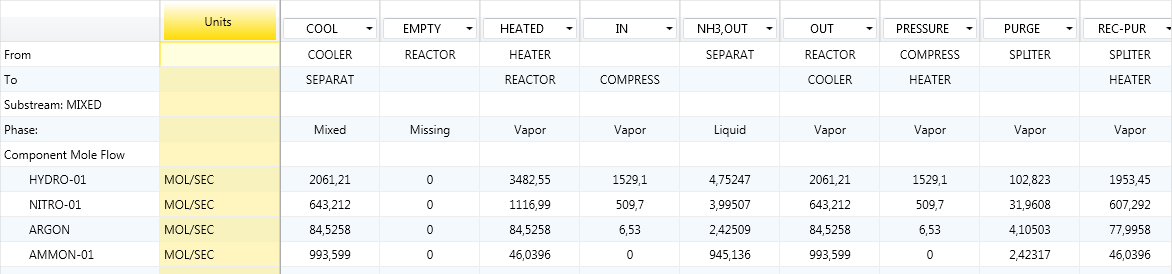
\includegraphics[scale=0.5]{RK-ASPEN.png}
	\end{center}
	\caption{Modèle \texttt{RK-ASPEN}, $750\si{\kelvin}$, $270\si{\bar}$, 5\%}
	\label{fig:RK-ASPEN}
\end{figure}

\begin{figure}[h!]
	\begin{center}
		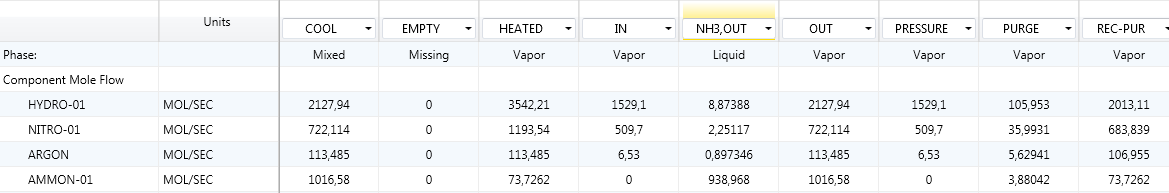
\includegraphics[scale=0.5]{PSRK.png}
	\end{center}
	\caption{Modèle \texttt{PSRK}, $750\si{\kelvin}$, $270\si{\bar}$, 5\%}
	\label{fig:PSRK}
\end{figure}

\begin{figure}[h!]
	\begin{center}
		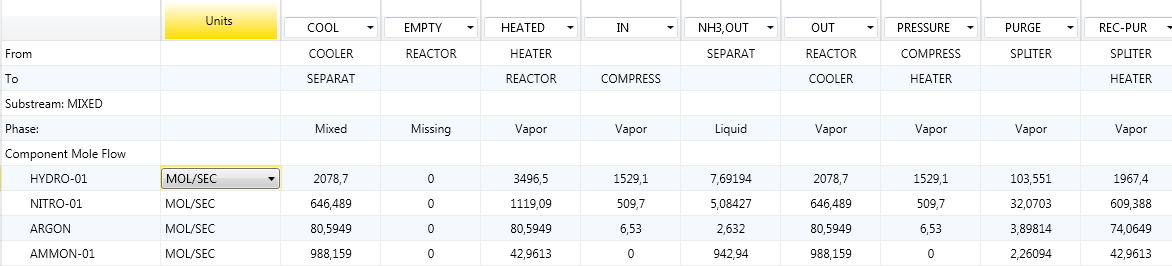
\includegraphics[scale=0.5]{SRK,750,270,5.png}
	\end{center}
	\caption{Modèle \texttt{SRK}, $750\si{\kelvin}$, $270\si{\bar}$, 5\%}
	\label{fig:SRK,750,270,0.05}
\end{figure}

\begin{figure}[h!]
	\begin{center}
		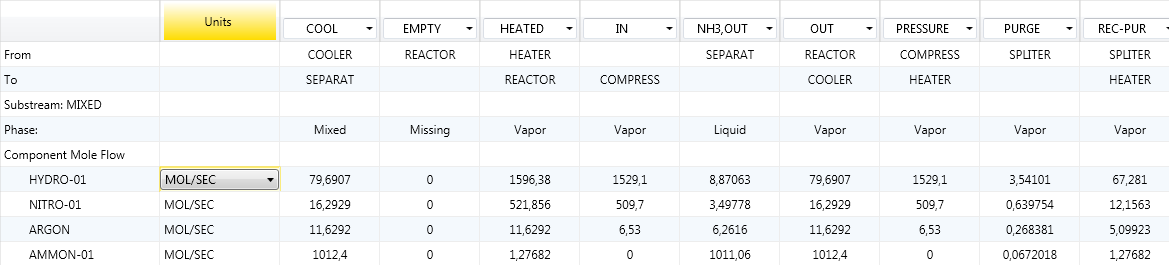
\includegraphics[scale=0.5]{SRK,500,270.png}
	\end{center}
	\caption{Modèle \texttt{SRK}, $500\si{\kelvin}$, $270\si{\bar}$, 5\%}
	\label{fig:SRK,500,270,0.05}
\end{figure}

\begin{figure}[h!]
	\begin{center}
		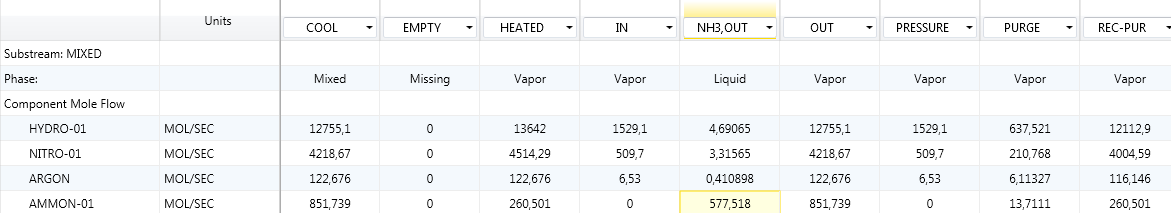
\includegraphics[scale=0.5]{SRK,1000,270.png}
	\end{center}
	\caption{Modèle \texttt{SRK}, $1000\si{\kelvin}$, $270\si{\bar}$, 5\%}
	\label{fig:SRK,1000,270,0.05}
\end{figure}

\begin{figure}[h!]
	\begin{center}
		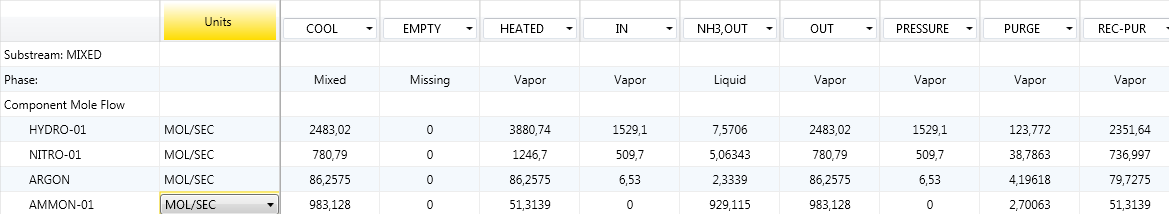
\includegraphics[scale=0.5]{SRK,750,220.png}
	\end{center}
	\caption{Modèle \texttt{SRK}, $750\si{\kelvin}$, $220\si{\bar}$, 5\%}
	\label{fig:SRK,750,220,0.05}
\end{figure}

\begin{figure}[h!]
	\begin{center}
		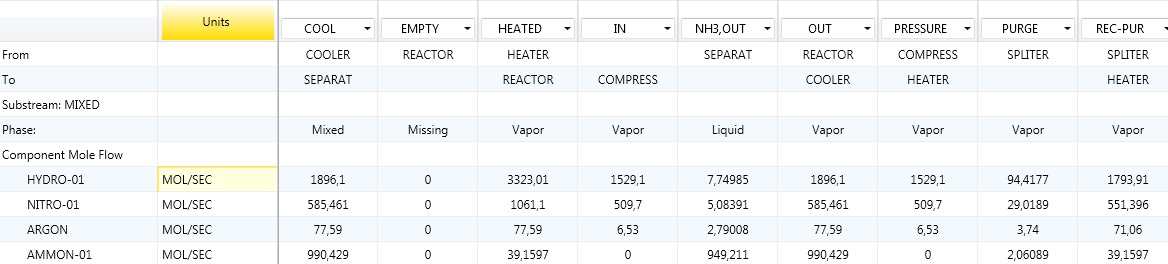
\includegraphics[scale=0.5]{SRK,750,300.png}
	\end{center}
	\caption{Modèle \texttt{SRK}, $750\si{\kelvin}$, $300\si{\bar}$, 5\%}
	\label{fig:SRK,750,300,0.05}
\end{figure}

\begin{figure}[h!]
	\begin{center}
		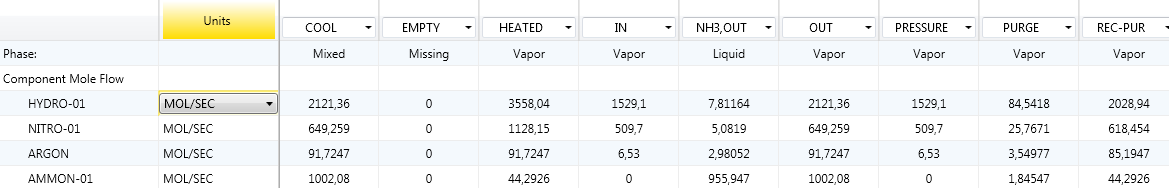
\includegraphics[scale=0.5]{SRK,750,270,4.png}
	\end{center}
	\caption{Modèle \texttt{SRK}, $750\si{\kelvin}$, $270\si{\bar}$, 4\%}
	\label{fig:SRK,750,270,0.04}
\end{figure}

\begin{figure}[h!]
	\begin{center}
		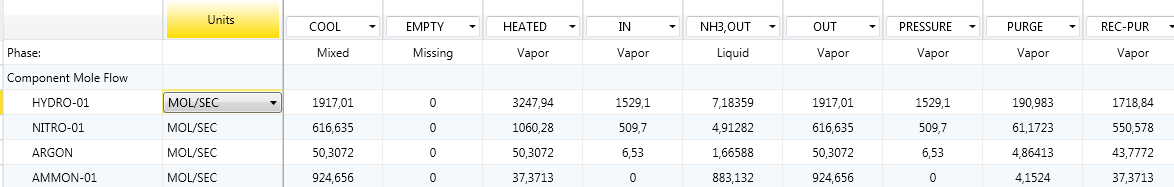
\includegraphics[scale=0.5]{SRK,750,270,10.png}
	\end{center}
	\caption{Modèle \texttt{SRK}, $750\si{\kelvin}$, $270\si{\bar}$, 10\%}
	\label{fig:SRK,750,270,0.1}
\end{figure}

\begin{figure}[h!]
	\begin{center}
		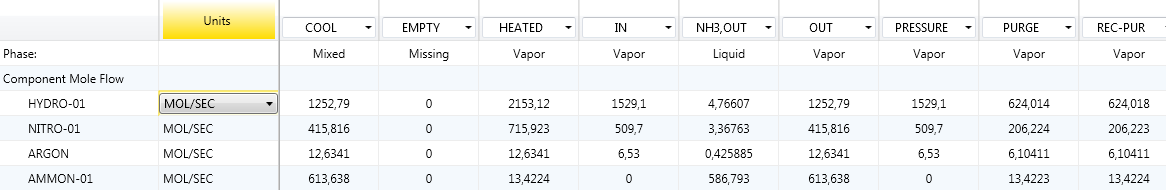
\includegraphics[scale=0.5]{SRK,750,270,50.png}
	\end{center}
	\caption{Modèle \texttt{SRK}, $750\si{\kelvin}$, $270\si{\bar}$, 50\%}
	\label{fig:SRK,750,270,0.5}
\end{figure}

\begin{figure}[h!]
	\begin{center}
		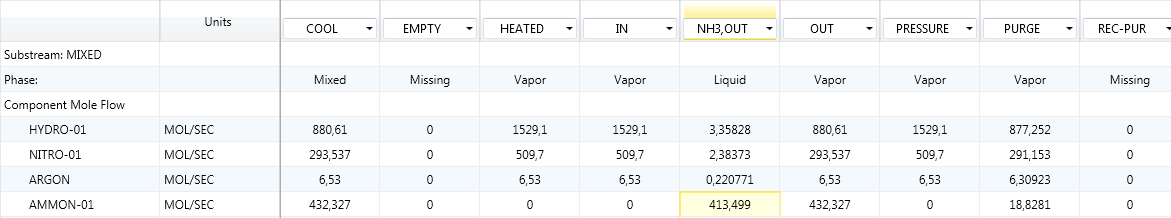
\includegraphics[scale=0.5]{SRK,750,270,100.png}
	\end{center}
	\caption{Modèle \texttt{SRK}, $750\si{\kelvin}$, $270\si{\bar}$, 100\%}
	\label{fig:SRK,750,270,1}
\end{figure}

\section{Outil de calcul: codes \textsc{Matlab}}




\printbibliography
\end{document}



\chapter{T\^ache 4}
%Quels sont les dangers présentés par les substances mises en œuvre durant la synthèse de l’ammoniac ?
\section{Dangers présentés les composés}

On retrouve $6$ gaz présents dans le réacteur. 
Certains ne présentent que peu de danger, 
d'autres peuvent provoquer d'importants dégats en cas de combustion.

\begin{itemize}	
	\item L'hydrogène est un gaz extrêmement inflammable et peut provoquer de grosses 
		explosions en cas de combustion. C'est le principal danger lié à sa présence. 
		En cas d'accumulation d'hydrogène dans une pièce ou un batiment, 
		sa présence peut provoquer un environnement déficient en oxygène et 
		donc provoquer la suffocation.

	\item  L'argon est présent naturellement dans l'air et n'est dangereux qu'en 
		quantités importantes. Il peut alors provoquer la suffocation.

	\item  L'azote est également naturellement présent dans l'air et n'est pas plus 
		dangereux que l'argon.

	\item  L'ammoniac est inflammable et peut donc provoquer une explosion en cas 
		d'accumulation et de combustion.

	\item  L'helium peut provoquer l'asphyxie en cas de concentration trop élevée.

	\item  Le méthane est inflammable et présente un danger d'explosion en cas 
		d'accumulation et de combustion. Il y a également un risque d'asphyxie en 
		cas d'accumulation simple.
\end{itemize}

\section{Circulation des flux de matière}

Les PDF et PID se trouvent à la fin du rapport dans l'annexe \ref{sec:fluxes}.



\section{Étude des dangers et catastrophes potentiels}


\paragraph{1} Imaginons que pour une quelconque raison, il y ait une fuite de gaz inflammable, 
de l'hydrogène par exemple. Le gaz se propagerait alors dans l'atmosphère à 
une pression de $150\si{\bar}$ et à une température de $180\si{\celsius}$. 
Il s'enflammerait directement, créant ainsi une augmentation rapide de la température. 
Les canalisations, chauffées par les flammes, verraient leur pression interne augmenter 
brutalement. Les canalisations se déchireraient, entraînant la libération d'hydrogène 
supplémentaire, provoquant ainsi une déflagration.

Nous pourrions éviter le déchirement des canalisations en utilisant des disques de rupture 
au niveau de celles-ci. Si la pression interne dépasse un certain seuil, le disque de rupture 
se rompt, libérant le gaz, mais évitant la destruction des tuyauteries.

\paragraph{2} Prenons maintenant le cas où un problème survient au niveau du réacteur 
de synthèse de l'ammoniac. La réaction de synthèse

\begin{equation}
	\ce{\frac{3}{2} H2_{(g)} + \frac{1}{2} N2_{(g)} <=> NH3_{(g)}}
	\label{eq:synthesis}
\end{equation}

est une réaction exothermique ($-45.9\si{\kilo\joule}$ à $298\si{\kelvin}$). 
Elle dégage donc beaucoup de chaleur, qu'il faut traiter afin d'éviter 
une hausse trop importante de la température au sein du réacteur. 
En faisant circuler les gaz de synthèse \ce{H2 \, et \, N2},  
qui sont à $180\si{\celsius}$, dans les parois du réacteur, 
ceux-ci vont absorber une partie de la chaleur produite par la réaction. 
Nous nous apercevons donc que s'il y a une défaillance au niveau du système 
de refroidissement, par exemple si l'entrée des gaz de synthèse est bouchée, 
la température du réacteur va augmenter brusquement. Etant donné que le volume est fixe, 
la pression va augmenter proportionnellement à la température, 
jusqu'à ce qu'elle dépasse la limite supportable par les parois du réacteur. 
A ce moment-là, le réacteur explose sous l'effet de la pression.

Pour éviter cela, il faut équiper le réacteur d'une soupape de sécurité, qui permettrait d'évacuer une partie du gaz afin de stabiliser la pression interne du réacteur. 
Nous pouvons également faire en sorte que le couvercle du réacteur cède en premier en cas de surpression, nous limiterions de cette manière fortement les dommages occasionnés.

\paragraph{3} Etudions maintenant le cas d'un blackout électrique. 
L'installation est soudainement privée d'électricité. 
Les compresseurs vont donc s'arrêter, et l'apport en réactifs au niveau 
du réacteur va donc s'arrêter.
La réaction va continuer jusqu'à ce que les pressions au niveau des tuyauteries 
des réactifs et de l'ammoniac s'équilibrent.
La synthèse de l'ammoniac diminue la pression car elle réduit le nombre de moles 
de gaz présent, mais est exothermique, et puisque le refroidissement est effectué 
par les réactifs, et que le système n'est plus alimenté, le réacteur va chauffer.
Il va également falloir redémarrer le réacteur une fois l'élecricité rétablie. 
Le réacteur doit avoir le temps de refroidir afin d'éviter 
que la température ne soit trop élevée lors du redémarrage. 
Il sera cependant nécessaire de purger ou préchauffer le réacteur si
la température du réacteur est trop basse car la réaction ne se fera pas.

Nous pouvons éviter tout problème en ayant des générateurs sur site capable 
de délivrer de l'électricité en cas de blackout jusqu'à ce que 
le courant soit rétablit. 

\section{Soupape de sécurité sur le réacteur de synthèse de l'ammoniac}

% Pourquoi n’y a-t-il pas de soupape de sécurité ou de disque de rupture (les deux types 
% de dispositifs servent à protéger un équipement ou une ligne contre les surpressions) 
% sur le réacteur de synthèse du NH3 ?

Un disque de rupture est un dispositif de sécurité qui sert à protéger les installations 
contre les surpressions.
La réaction de synthèse de l'ammoniac est la réaction \ref{eq:synthesis}.
On remarque immédiatement qu'il y a une diminution du nombre de moles de gaz (d'un facteur 2) 
lorsque de l'ammoniac est produit. La loi des gazs parfait nous indique que la pression
exercée par un gaz est directement proportionnelle à son nombre de moles.
Une surpression n'est pas envisageable pour cette réaction, 
il n'y a donc pas besoin de disque de rupture sur ce réacteur.

\section{Disque de rupture sur l'échangeur \textsc{124-mc}}
% Pourquoi y a-t-il des disques de rupture sur l’échangeur 124-MC ?

L'échangeur 124-C est un dispositif permettant de transférer de la chaleur d'un fluide
vers un autre, sans que ceux-ci ne se mélangent.
On a donc un flux \emph{chaud} et un flux \emph{froid}. Le flux froid va recevoir de 
l'énergie thermique et sa température va augmenter, il faut alors prévoir des disques 
de rupture au cas où la température dépasse une certaine limite qui produirait une 
supression du gaz et pourrait endommager, voire déchirer, la paroi.
Théoriquement, le flux chaud n'a pas besoin de disque de rupture parce que le gaz qu'il 
transporte ne peut que diminuer de volume. Cependant, on peut toujours considérer le cas
d'un apport soudain et imprévu de chaleur comme une explosion extérieure, qui produirait
une augmentation de température et par conséquent de pression. 
Il devient alors nécessaire d'avoir des disques de rupture dans les deux sens de l'échangeur.


\section{Circulation des flux de matières - \textsc{pdf} et \textsc{pid}'s}
\label{sec:fluxes}

\begin{center}
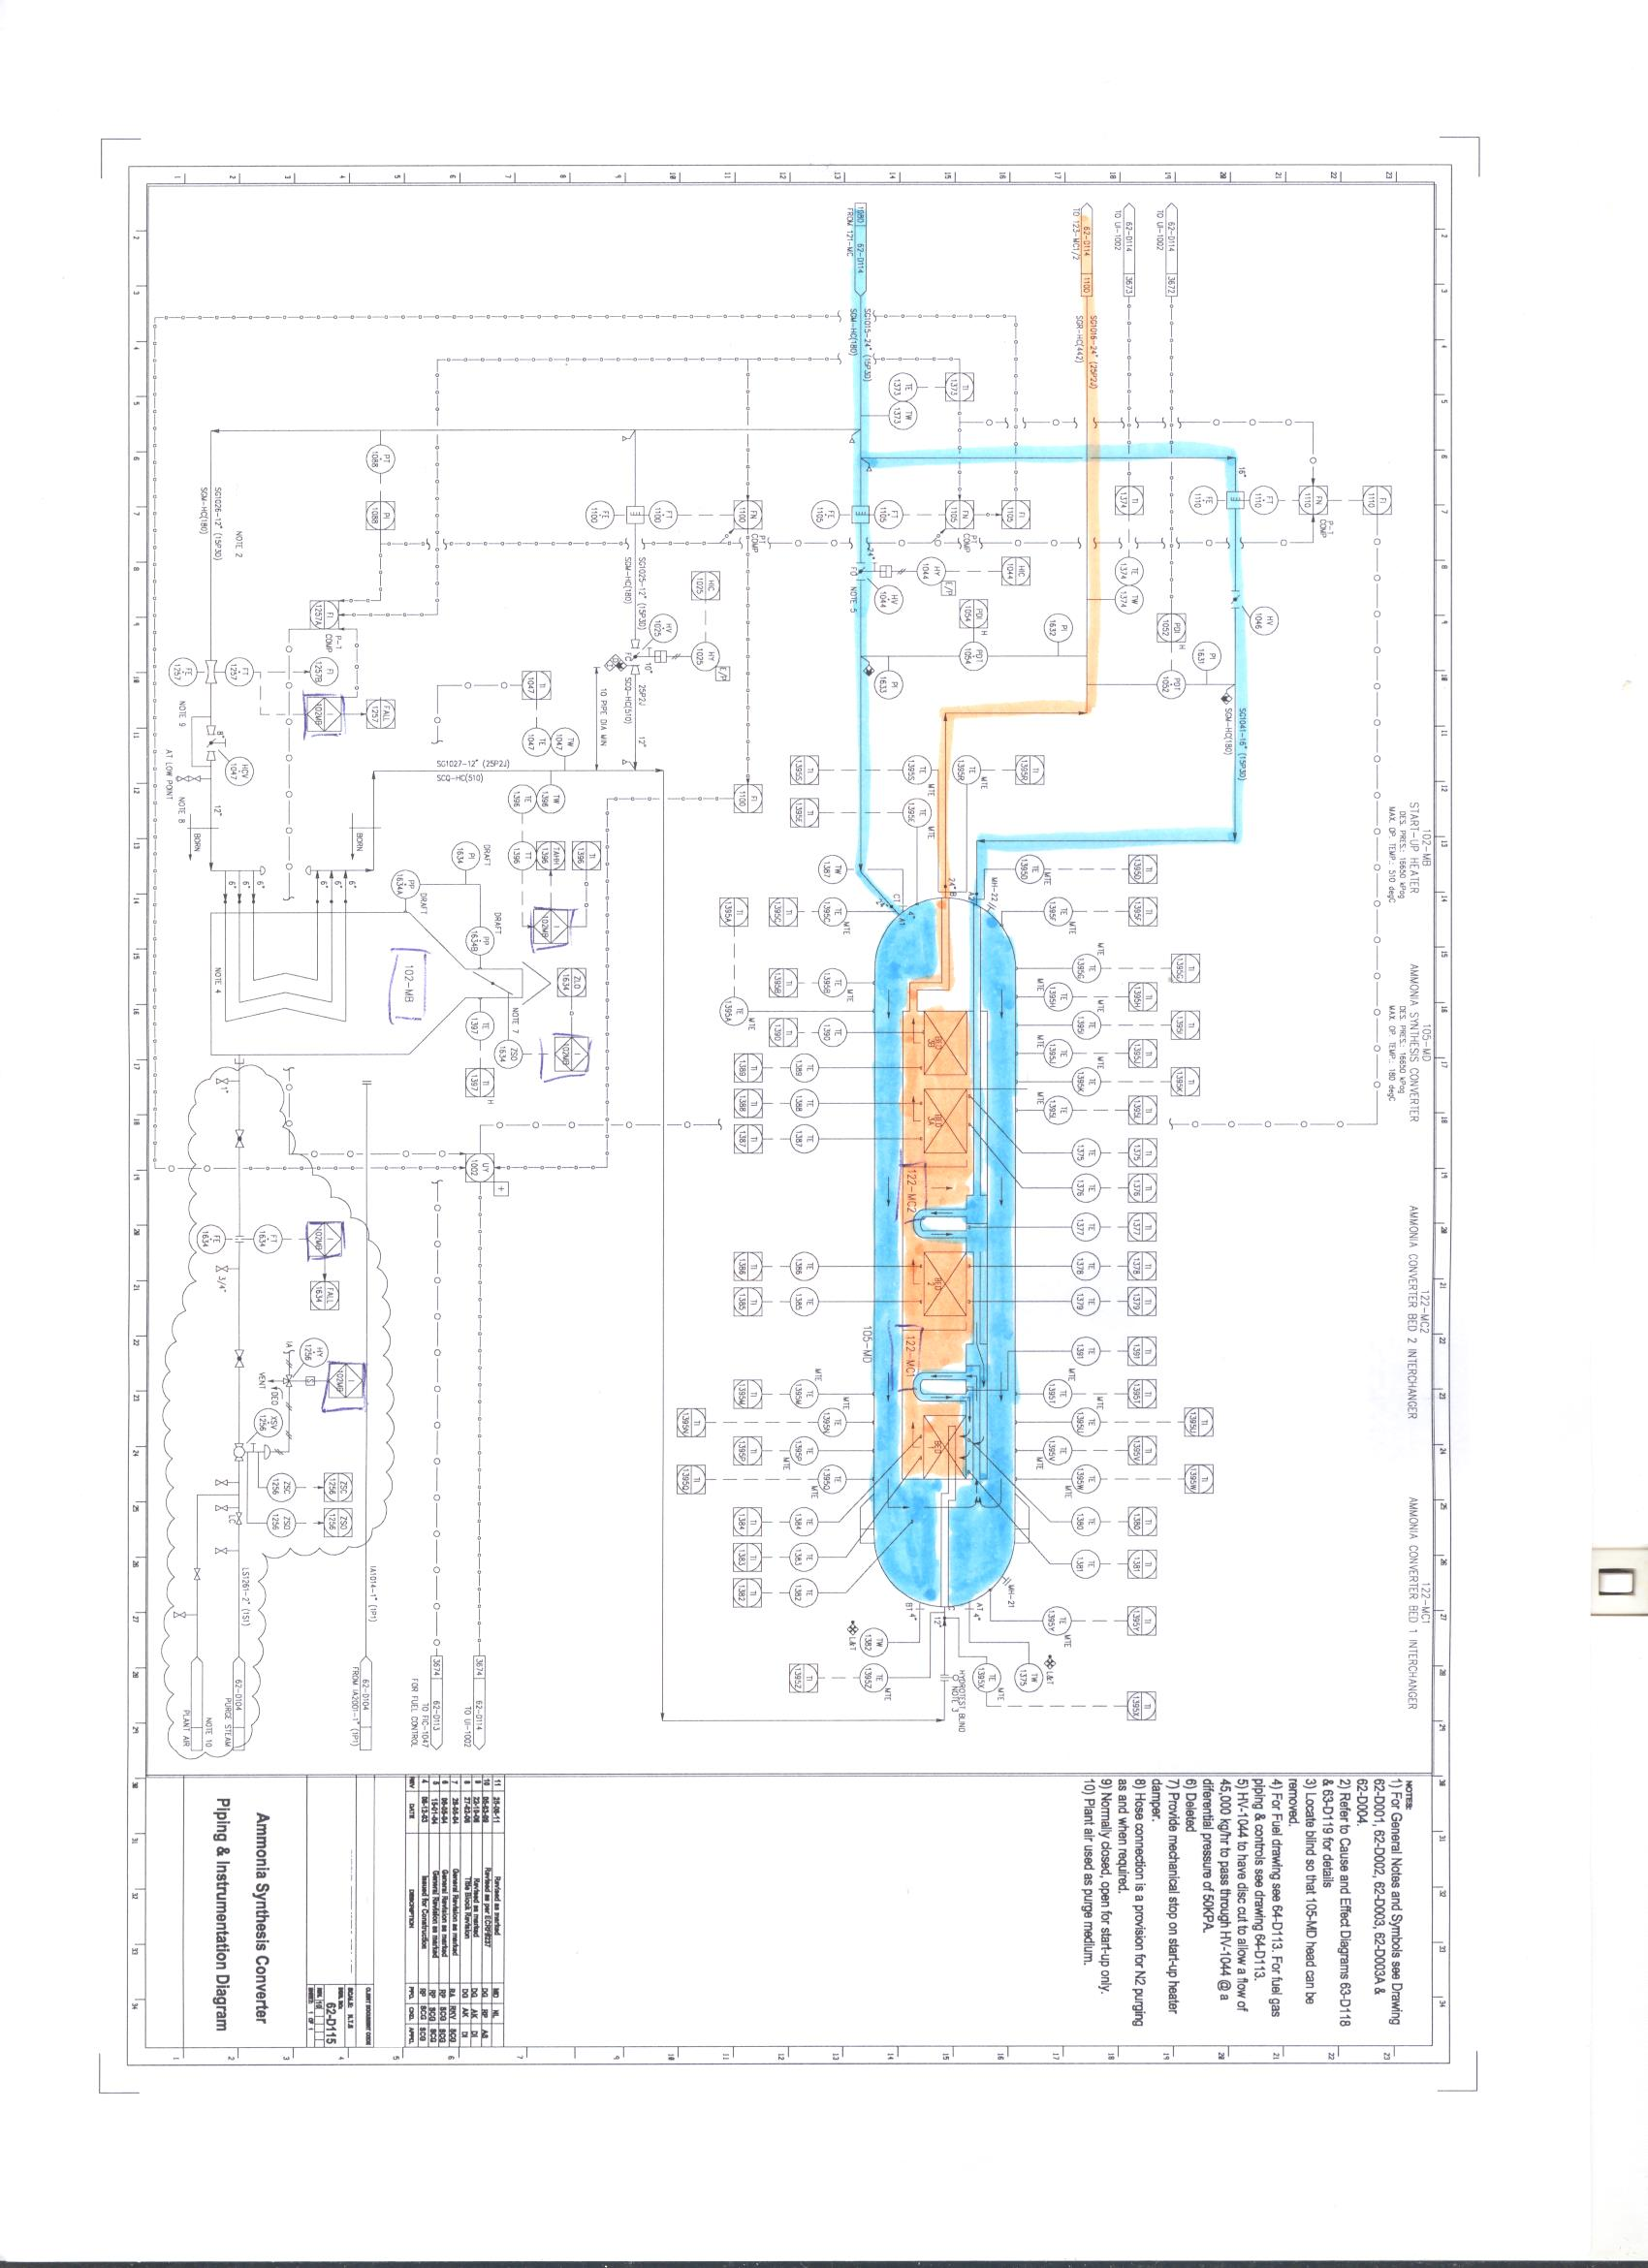
\includegraphics[scale=0.7]{../tache4/img/scan1.jpg}

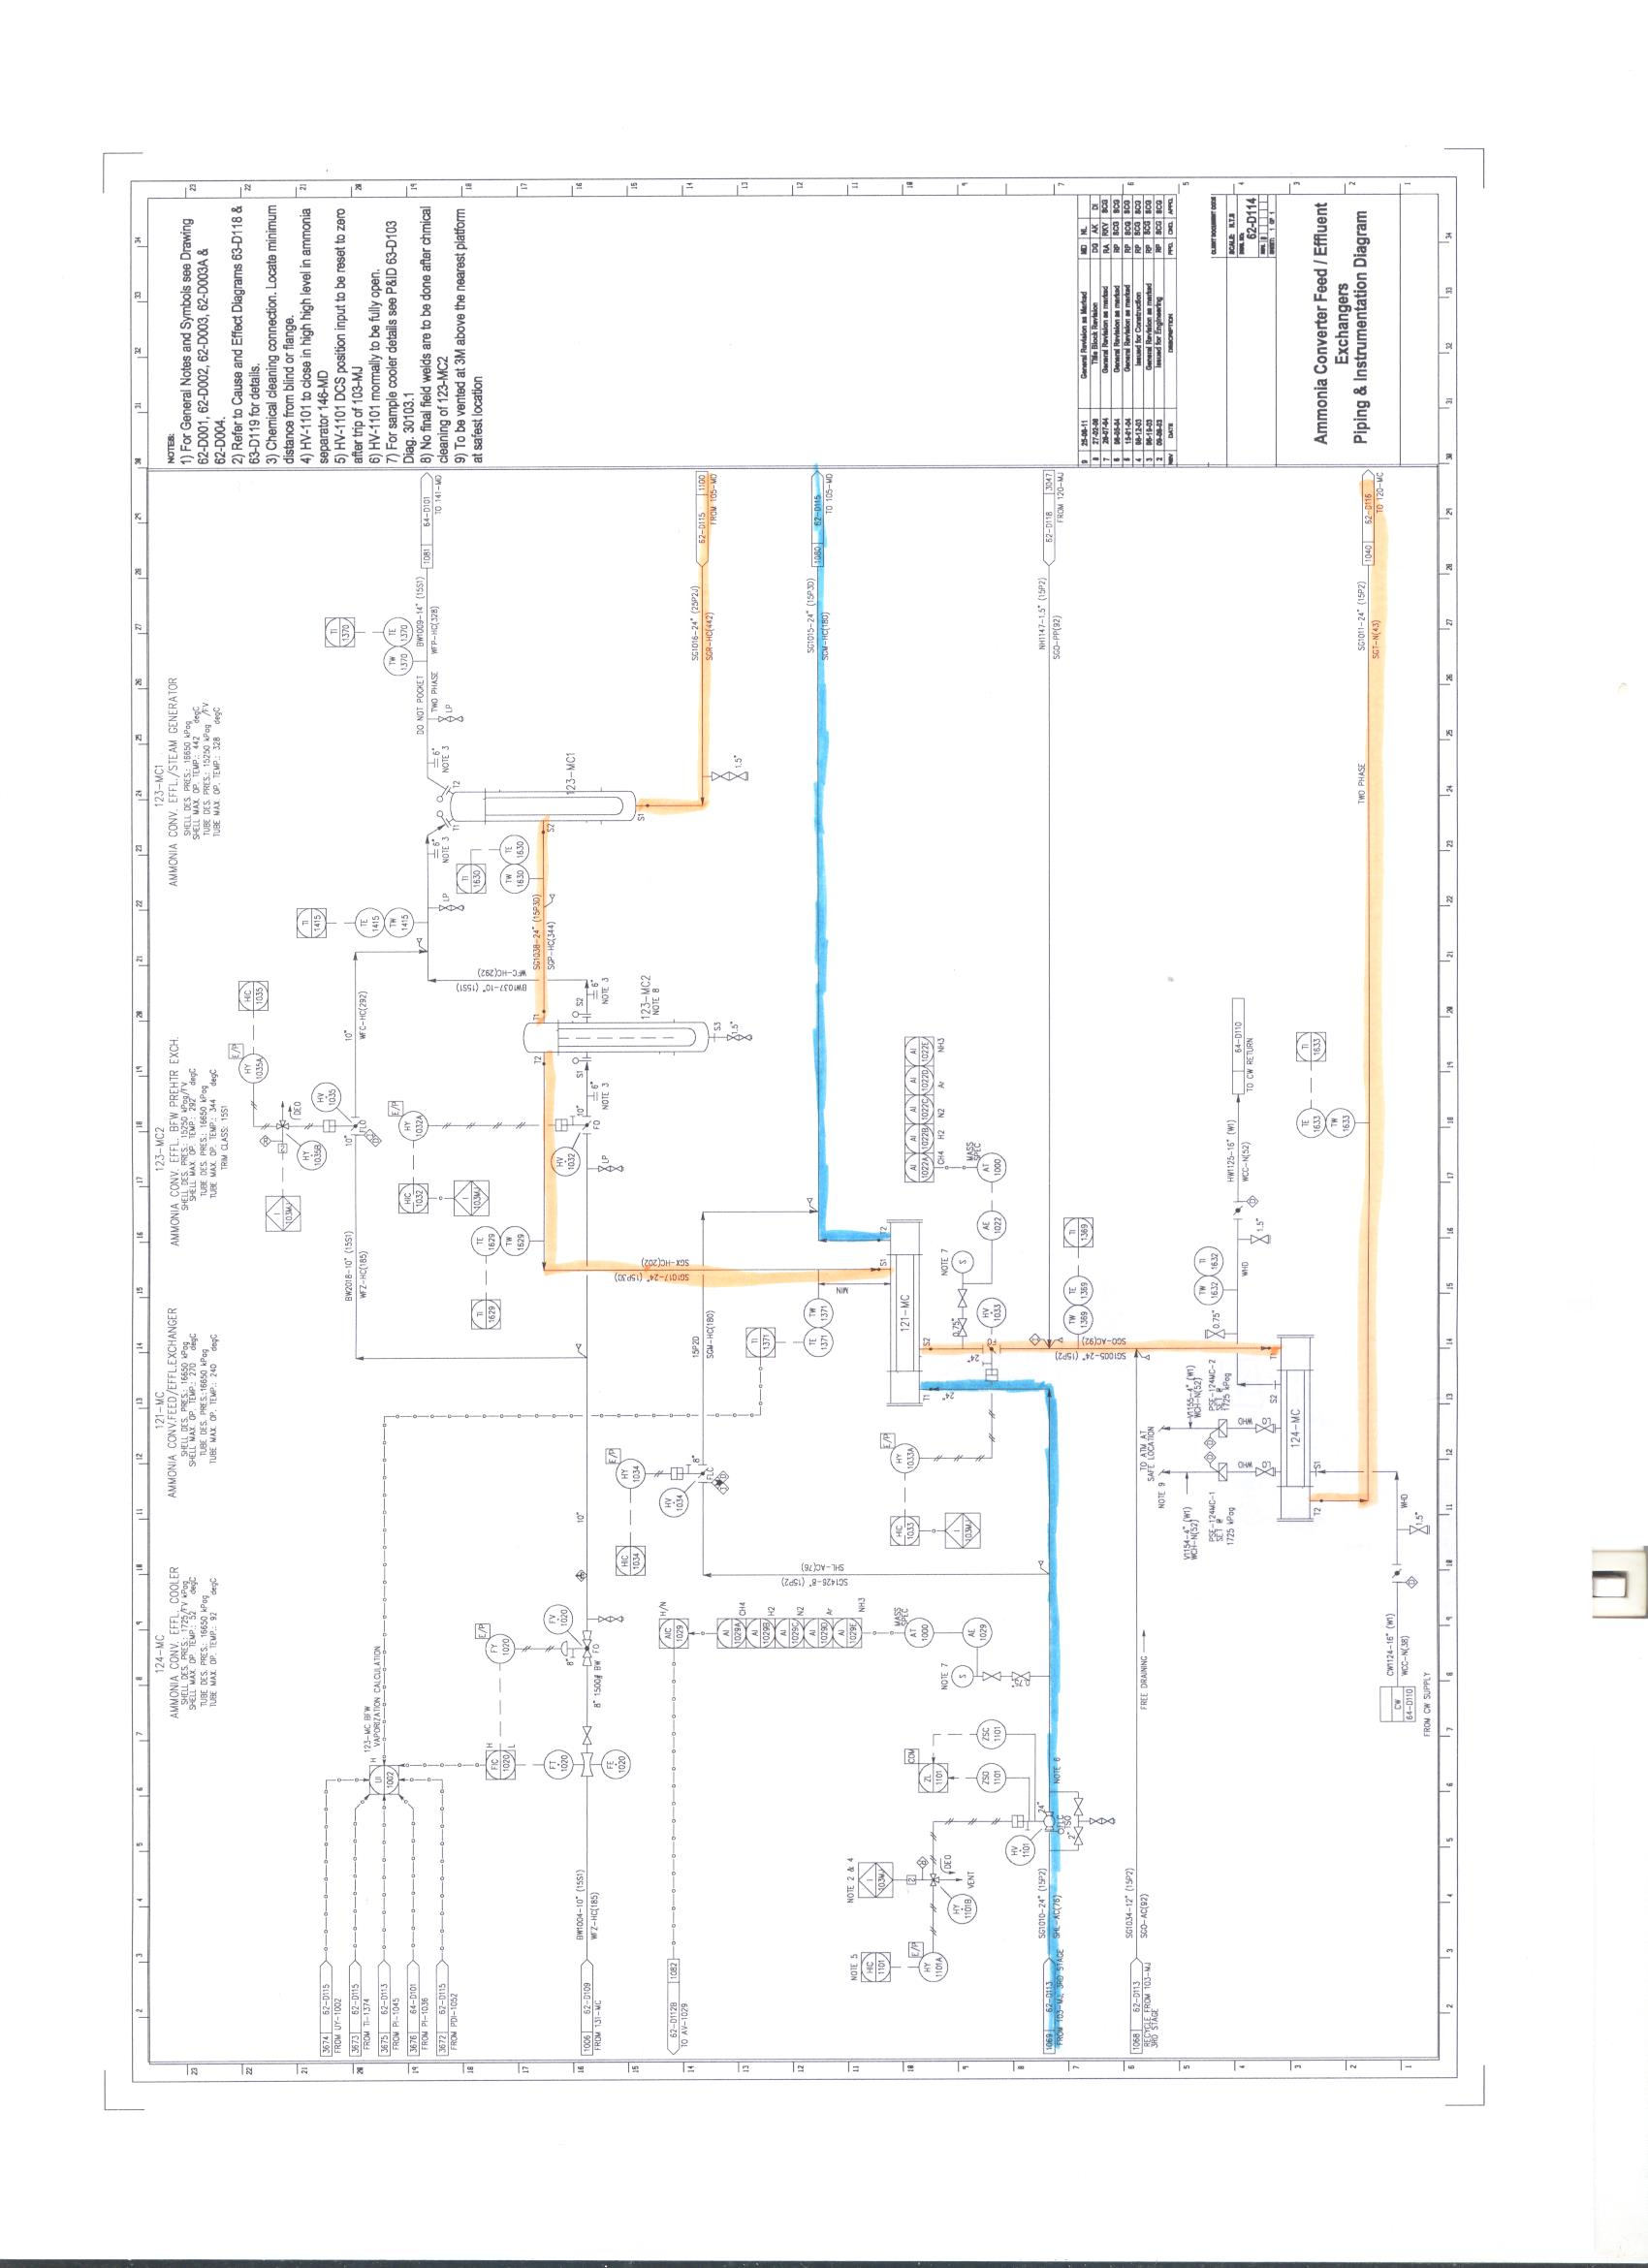
\includegraphics[scale=0.7]{../tache4/img/scan2.jpg}

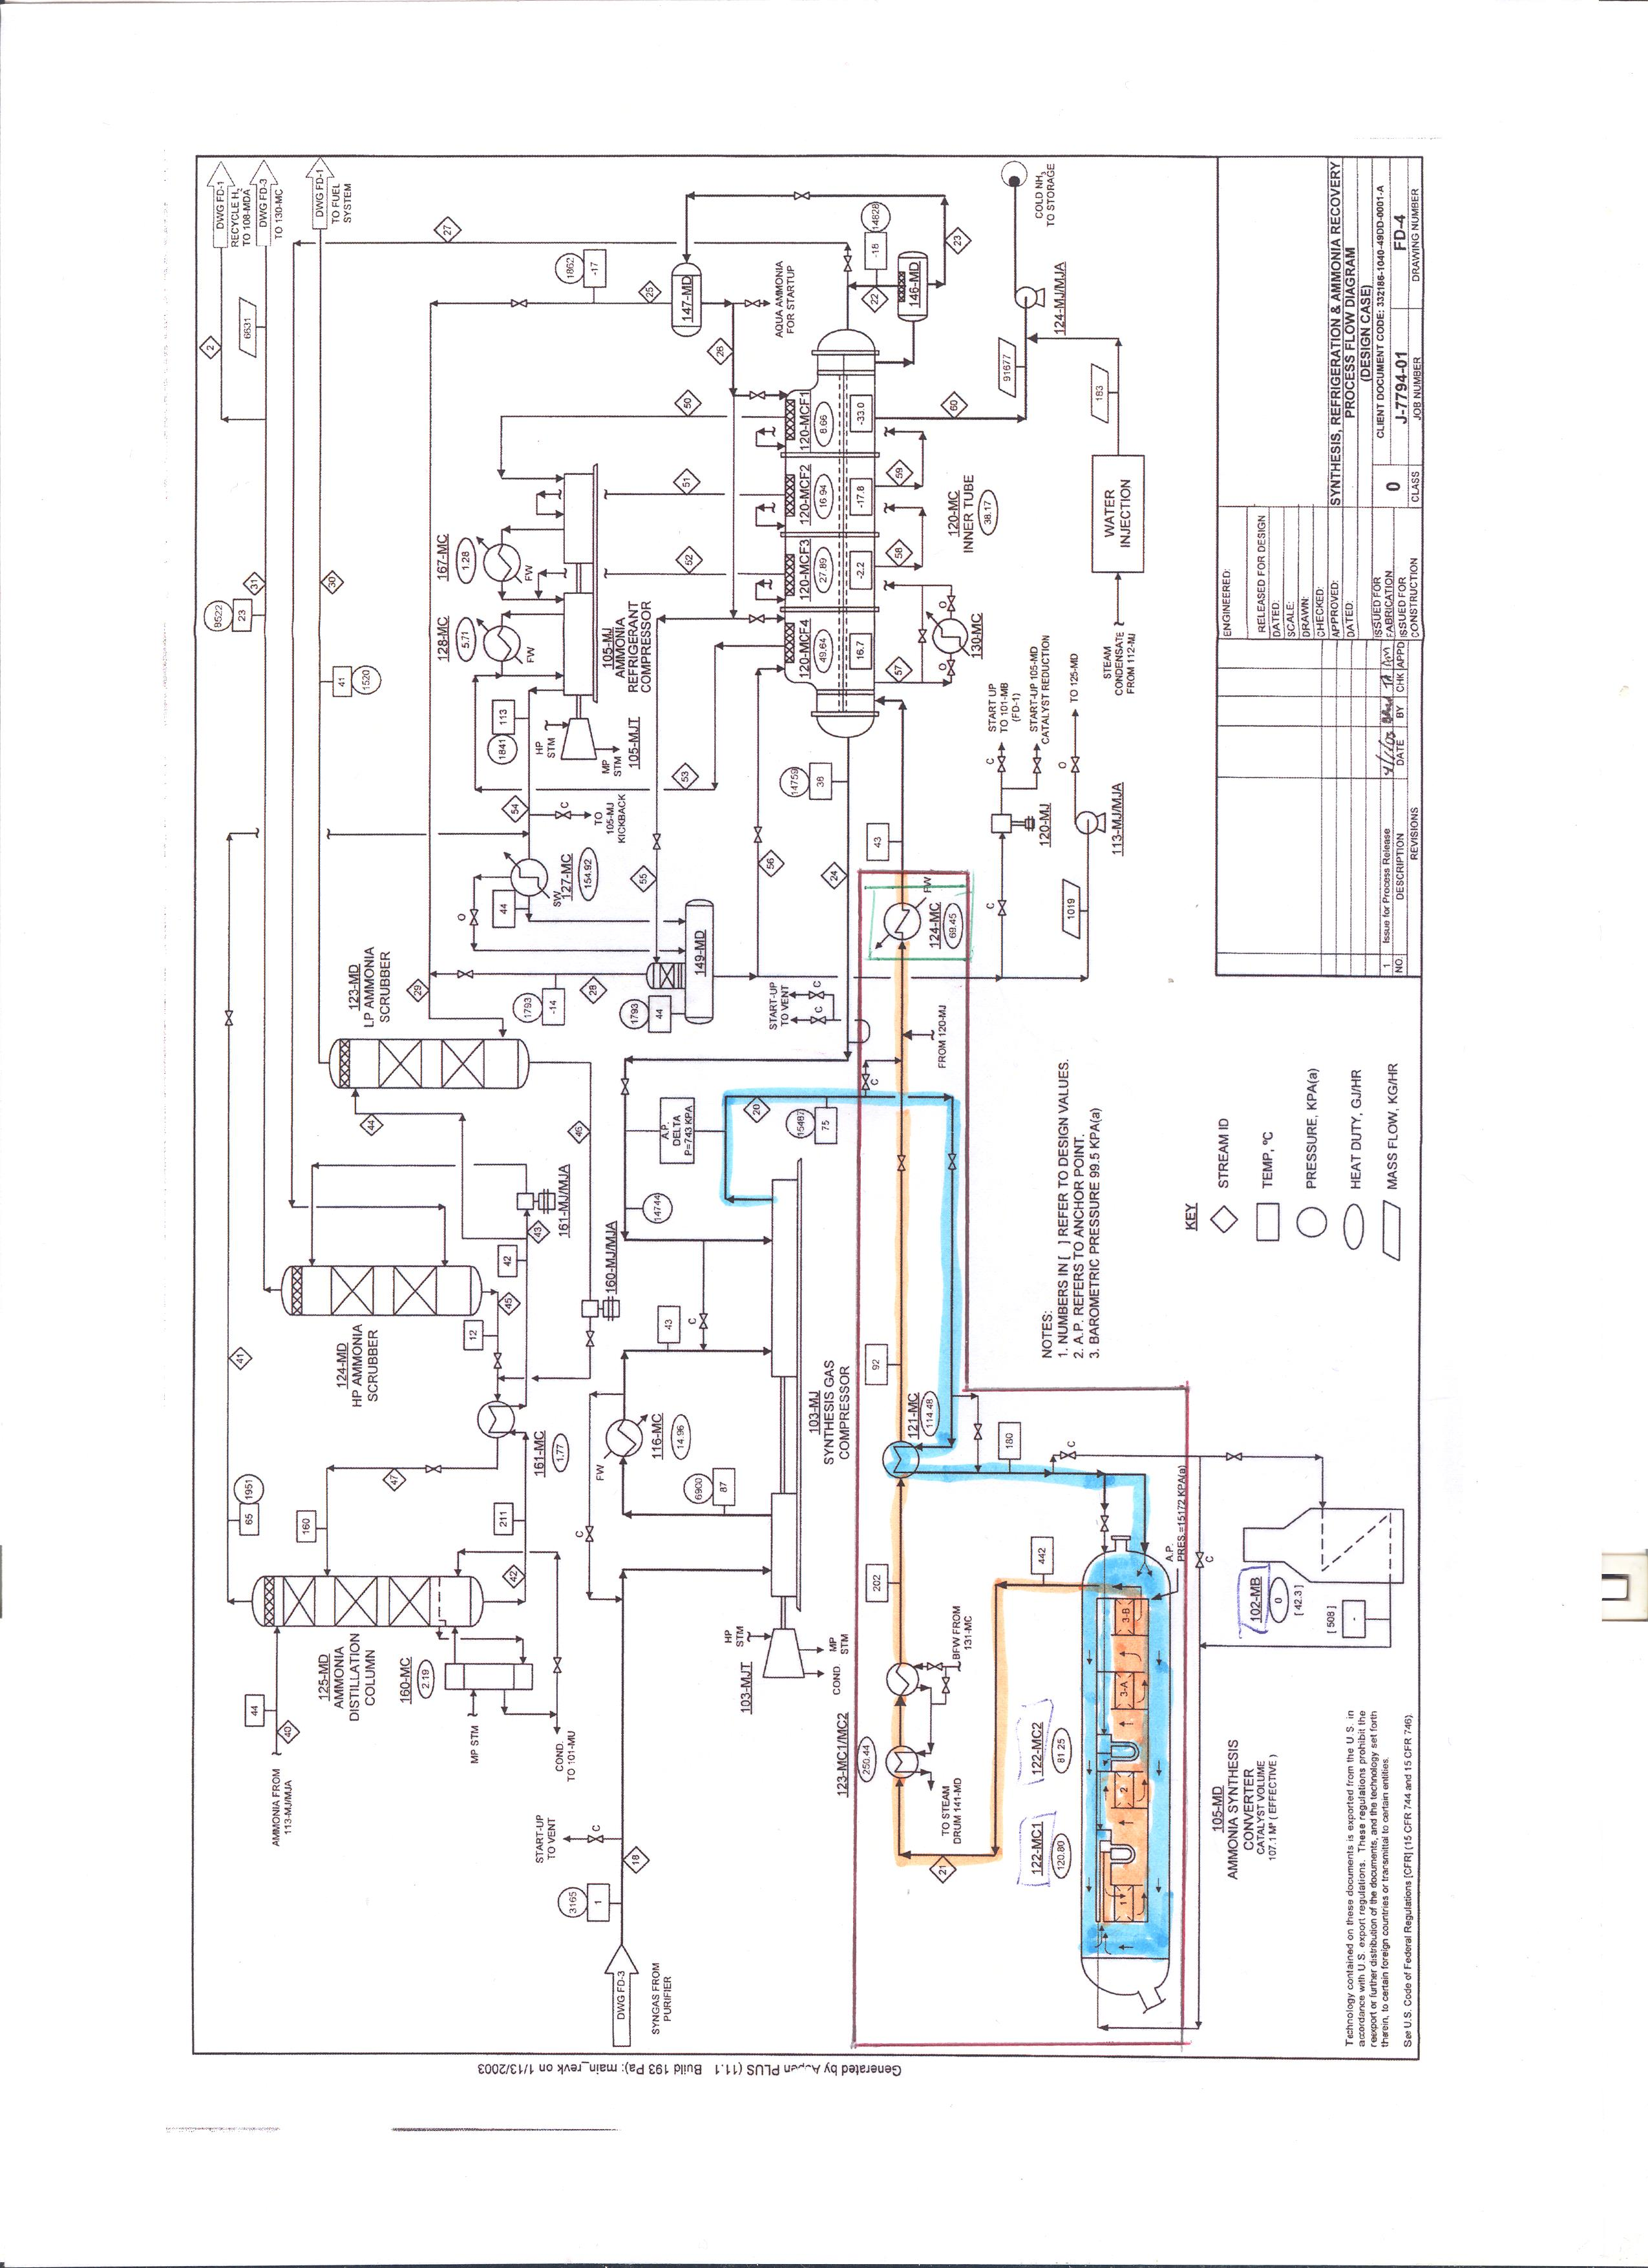
\includegraphics[scale=0.7]{../tache4/img/scan3.jpg}
\end{center}



\chapter{T\^ache 5}
Pour la t\^ache 5, il nous était demandé de dimensionner une soupape de sécurité
pour un tank contenant de l'ammoniac. Pour celà, nous avons recu quelques informations:

\begin{itemize}

\item Forme du tank: cylindrique vertical à extrémités hémisphériques. Tank au sol.
\item Hauteur totale du tank: $12 \si{\metre}$
\item Niveau de \ce{NH3} liquide dans le tank: $8\si{\metre}$
\item Diamètre du tank: $6 \si{\metre}$
\item Température normale de stockage: $20 \si{\degreeCelsius}$
\item Pression de design: $15 \barg$
\item Cp/Cv du \ce{NH3}: $1.33$; Facteur de compressibilité Z: $1.0$
\item La soupape sera une soupape conventionnelle et la contrepression sera nulle.
\item L’usine est munie de systèmes de drainages des fuites 
	et d’un équipement moderne de lutte contre l’incendie.
\end{itemize}

Nous avons également à notre disposition deux graphes donnant respectivement 
les pressions de stockage de l'ammoniac et de l'enthalpie de vaporisation 
en fonction de la température.

\paragraph{Remarque}
A travers cette section nous utilisons l'unité \barg, 
qui correspond à la pression supérieur à la pression atmosphérique.
On a donc:
\[ p [\barg] = p [\si{\bar}] - 1 \]

% Quelle est la pression normale de stockage ?
\section{Pression normale de stockage} 
La pression normale de stockage est de $7.8 \barg$ à $20\si{\celsius}$ 
(température normale de stockage). Nous avons obtenu ces résultats sur base des
graphiques que nous avions reçus.

% Quelle sera la pression de stockage en été (30°C) ?
\section{Pression de stockage en été} 
La pression de stockage en été est de $10.625 \barg$ à $30\si{\celsius}$.

% Quel sera la pression maximale de tarage de la soupape de sécurité ?
\section{Pression maximale de tarage de la soupape} 
La pression maximale de tarage de la soupape de sécurité vaut 
\[ 121\% \cdot p_{\text{design}} = 18.15 \barg \]

% Dimensionner la soupape pour cette pression de tarage.
%     -	Quelle sera la pression durant la décharge ?
%     -	Quelle sera la température du liquide durant la décharge via la soupape ?
%     -	Quelle sera la taille de la soupape nécessaire ?
\section{Dimensionnement de la soupape} 
La pression durant la décharge sera de $19.16325 \si{\bar}$. 
Cette pression est fort élevée car nous considérons le cas d'un incendie au niveau du réservoir. 
La température du gaz durant la décharge sera de $50\si{\celsius}$. 
Nous aurons besoin d'une soupape d'une section de $730\si{\milli\meter\squared}$ 
ou $1.13 \, \text{inch}^2$. Ceci correspond à une PSV de type $2J3$
\[ C = 0.03948 \cdot \sqrt{1.33 \cdot \frac{2}{2.33}^{\frac{2.33}{0.33}}} \]
\[ W = 43200 \cdot 1 \cdot 143.634^{0.82} \]
\[ A = \frac{W}{C \cdot 0.975 \cdot 20.071 \cdot 1 \cdot 1} \cdot \sqrt{\frac{323.15}{17}} \]

\section{Effet de l'augmentation de la pression de tarage de 5 à 20 barg pour une pression de design de 20 barg} 
Si la pression de design est à $20\barg$, nous pouvons augmenter la pression de tarage à \[ 121\% \cdot p_{\text{design}} = 24.2\barg \]

Nous recalculons A avec la pression et température plus élevées,
et obtenons que la soupape doit avoir une section de $590\si{\milli\meter\squared}$
ce qui nous donne $0.9118 \, \text{inch}^2$. Ceci correspond à une PSV de type $2J3$ comme celle trouvée précédemment. Il n'y a donc pas d'intérêt
à augmenter la pression de design dans ces conditions.

% Pour la première pression de tarage, quelle est l’influence d’isoler thermiquement 
% le tank avec un isolant tel que le coefficient d’échange avec l’extérieur 
% soit réduit à une valeur de 10 W/m2.K ? 
\section{Isolation thermique du tank}
Nous isolons la cuve avec un isolant réduisant le coefficient d'échange de la cuve avec l'extérieur à 
$10 \si{\watt}/\si{\meter\squared} \cdot \si{\kelvin}$
On réduit donc le facteur environnemental à $F = 0.15$. 
Notre $W$ va donc être fortement réduit, et nous pouvons donc réduire la taille de la soupape à 
$110\si{\milli\meter\squared}$ ou $0.17 \, \text{inch}^2$. 
Cette PSV est du type $1E2$. L'ajout de l'isolant réduit donc fortement la taille de
la soupape requise.



\chapter{T\^ache 7}
\section{Visite de la station de biométhanisation de l’\textsc{aive} à Tenneville}

L’usine de biométhanisation permet de créer du \ce{CH4} à partir de déchets organiques,
principalement ménagers, mais aussi provenant de parcs à conteneurs, etc.

Premièrement, les déchets sont acheminés par camions au centre de Tenneville.
Avant que les déchets ne soient stockés dans un entrepôt, 
les camions passent à travers un portique afin 
d'y détecter la présence de déchets radioactifs. Ils sont ensuite pesés
puis déchargés dans le premier entrepôt.

Les déchets passent à travers un broyeur et sont acheminés par tapis roulant 
où des aimants permettent d’y retirer les déchets ferreux indésirables.
À cette étape, les déchets sont prêts à entrer dans le digesteur. 
Ce digesteur ressemble à un grand silo d’une capacité de $3000 \si{\meter\cubed}$.
Le principe est assez simple, des bactéries anaérobies vont commencer à digérer 
ces matières organiques en l’absence d’oxygène, ce qui crée du méthane. 
Le méthane sert à la production d’électricité et de chaleur (principe de cogénération).
L’usine est donc autosuffisante en termes d'électricité et de chauffage.
Le surplus  d’électricité est redistribué sur le réseau, et l’excédent de chaleur 
est utilisé pour le séchage de boue ainsi que dans d’autres usines de recyclage. 

Une fois la matière digérée, elle est compostée complètement jusqu’à l’obtention 
de terreau qui est revendu aux agriculteurs.
En cas de panne de moteur - ou tout autre problème dans le digesteur -
il y a une torchère qui permet du brûler tout surplus de méthane
et donc d'éviter tout excès dans le digesteur. Cela évite aussi de devoir 
libérer du méthane dans l’atmosphère.

Quelques chiffres :
\begin{itemize}
	\item Capacité de traitement : $39 000$ tonnes par an
	\item Production en électricité : équivalent à la consommation de $1500$ ménages
	\item Production de gaz : $55\%$ de \ce{CH4}, $44\%$ de \ce{CO2} + autres gaz
\end{itemize}

\section{Visite du centre Total Research Technology Feluy}

\subsection{Catalyse}
\label{subsec:catalyse}

L'utilisation d'un catalyseur est essentielle pour de nombreuses réactions industrielles 
effectuées aujourd'hui. De nombreuses réactions ne seraient même pas possibles sans 
l'utilisation d'un catalyseur.
 
Un catalyseur réduit l'énergie d'activation d'une réaction en affaiblissant les liens
électroniques des molécules devant réagir, ou en affaiblissant les liens entre les 
molécules des réactifs. Certains catalyseurs sont en pratique ``consommés'' durant 
la réaction (ex: emprisonnés dans les molécules) et d'autres ne sont simplement pas 
affectés par les réactions. 

Dans de nombreuses réactions, les catalyseurs ont également d'autres rôles. 
Suivant le catalyseur utilisé, certaines réactions seront favorisées au détriment 
d'autres (il faut donc trouver un catalyseur favorisant la réaction voulue). 
Le catalyseur peut également déterminer la structure des molécules obtenues lors 
d'une cristallisation. Suivant le catalyseur utilisé lors de la synthèse de polyéthylène,
on obtiendra une poudre fine ou de plus gros grains,
deux structures ayant des applications différentes.
 
Trouver le bon catalyseur est donc essentiel dans la chimie moderne.
 
\subsection{Unités Pilotes}
 
Le développement de nouveaux procédés ou catalyseurs commence tout d'abord en laboratoire,
ou de microréacteurs permettent de tester la viabilité des nouveaux développements.
Si un catalyseur ou un procédé est considéré comme intéressant,
il va ensuite être testé dans une unité pilote. 

Différentes réactions demandent différents réacteurs,
et le réacteur idéal pour une nouvelle réaction est déterminé en laboratoire.
 
Les unités pilotes sont des réacteurs industriels réduits utilisés pour tester de
nouvelles réactions ou de nouveaux procédés. Les unités pilotes sont beaucoup plus
modulables que les unités industrielles. Celles-ci vont permettre de détecter
d'éventuels problèmes qui sont passés inaperçus lors des tests en laboratoires,
ainsi que de déterminer les conditions idéales pour l'utilisation des nouvelles réactions.
Si un nouveau produit (nouvelle structure ou autre) est considéré comme intéressant,
les unités pilotes vont permettre de produire une quantité limitée de ce nouveau
produit afin de fournir des échantillons à des partenaires commerciaux.
Elles évitent ainsi de devoir reconfigurer des plants de grande taille.

\section{Laboratoire d’électrolyse}

L'électrolyse de l'eau est un procédé qui permet de décomposer 
celle-ci en dioxygène et en dihydroègne, tous deux à l'état gazeux.

\begin{equation*}
	\ce{H2O_{(g)} <=> \frac{1}{2} \, O2_{(g)} + H2_{(g)}} 
\end{equation*}

Afin de produire du dihydrogène gazeux en quantités décentes, l'électrolyse de l'eau 
demande énormément d'énergie électrique (sous forme de courant). De plus, le rendement
de la réaction d'électrolyse de l'eau ne dépasse en général jamais les $50\%$.

Sur base des expérimentations effectuées en laboratoire, nous observons que pour un même volume de dihydrogène produit, 
plus l’intensité du courant est élevée, plus le temps nécessaire à la production
du dihydrogène est faible. En fait, le courant et le temps sont inversément proportionnels, 
et nous pouvons écrire la relation suivante :

\begin{equation*}
	It = \text{constante}
\end{equation*}

où I est l'intensité du courant électrique, et t, le temps écoulé. 
Cela montre bien que lorsqu'on augmente le courant, le temps diminue dans les mêmes proportions.

Calculons maintenant la puissance nécessaire pour produire tout l'hydrogène 
dont nous avons besoin pour un débit d'ammonicac de 1500 t/j.

En prenant une température de $1000 \si{\kelvin}$ pour le reformeur primaire, 
nous savons grâce à notre outil de calcul que pour produire 1500 t/j d'ammoniac, il faut $266,32 \si{\tonne}$ de dihydrogène 
par jour. Cela nous donne un débit massique de $184,944 \, \si{\kilo\gram/\minute}$.

Nous devons maintenant fixer trois paramètres pour le déroulement de la réaction d'électrolyse : le pH, la température et le courant.
La réaction d'électrolyse nécessite une puissance moins importante lorsque le pH tend vers 0. Mais un pH nul demande une grande quantité d'acide, nous allons donc nous contenter ici d'un pH = 1.
Par souci d'économie d'énergie, nous allons travailler à température ambiante, soit $20\si{\celsius}$.
Le dernier paramètre est le courant, que nous allons faire varier afin d'obtenir la quantité voulue d'hydrogène.
Par exemple, en appliquant un courant de $0,5 \si{\ampere}$, nous savons, grâce aux expériences faites en laboratoire, 
que nous produisons $4 \, \si{\milli\liter}$ de dihydrogène par minute. 
Considérons maintenant que le dihydrogène se comporte comme un gaz parfait, nous pouvons appliquer :

\begin{equation*}
	pV = mR^{*}T
\end{equation*}

et donc calculer la masse de dihydrogène, sachant que la réaction se déroule 
sous une température de $293,15 \si{\kelvin}$ et une pression de $1 \si{\bar}$. 
Nous obtenons ainsi qu'en faisant circuler un courant de $0.5 \si{\ampere}$, 
nous produisons $3,2824\e{-7} \, \si{\kilo\gram/\minute}$ de dihydrogène.

Pour atteindre un débit massique de $184,944 \, \si{\kilo\gram/\minute}$, 
il faut donc un courant électrique de $2,817\e{8} \si{\ampere}$. 
Nous savons grâce aux résultats du laboratoire que la tension électrique dépend quant à elle du pH. 
Pour un pH = 1, la tension appliquée par la source sera de 10 V.
Nous pouvons alors calculer la puissance électrique grâce à la relation suivante : 

\begin{equation*}
	P = UI
\end{equation*}

La puissance est donc égale à $2,817 \, \si{\giga\watt}$.

Cette puissance requise est énorme. L'électrolyse de l'eau demande 
beaucoup trop de puissance pour produire ce dont nous avons besoin. 
C'est pour cela que l'électrolyse est encore très peu utilisée à l'échelle industrielle. 
Il est donc préférable dans notre cas de se contenter du vaporeformage, 
malgré le fait qu'il émette du dioxyde de carbone.

\section{Visite du plant de Yara à Tertre}

Le plant de Yara fabrique des engrais et produit lui-même son propre ammoniac nécessaire
pour créer ces engrais. Avoir une production locale d'ammoniac permet non seulement 
d'éviter des coûts importants mais aussi d'éviter le transport de celui-ci car il 
peut s'avérer être toxique.

Tout d'abord, le réacteur où est synthétisé l'ammoniac est à une pression de $130 \si{\bar}$.
Comme décrit dans la section \ref{subsec:catalyse}, l'utilisation de catalyseurs dans la
production du méthane est fondamentale. Un catalyseur est utilisé lorsque la 
barrière énergétique pour qu'une réaction se produise est trop haute. Il va alors 
diminuer l'énergie d'activation sans modifier le chemin réactionnel.

Le diagramme de la figure \ref{fig:synthese} présente le fonctionnement simplifié 
des réacteurs de synthèse d'ammoniac. Il est important de préciser que le \emph{input}
est tout d'abord composé d'hydrogène et d'azote mais aussi de résidus de méthane, 
d'argon et d'hélium. Ceux-ci sont éliminés via différentes techniques 
de séparation (ex: par des membranes semi-perméables). 

\begin{figure}[h!]
	\begin{center}
		\begin{tikzpicture}
[node distance = 7em]

\tikzstyle{block} = [rectangle, draw, fill=blue!20, 
    text width=10em, text centered, rounded corners, minimum height=3em]
\tikzstyle{block2} = [rectangle, draw, fill=red!60, 
    text width=6em, text centered, minimum height=2em]
\tikzstyle{line} = [draw, -latex']
\tikzstyle{cloud} = [draw, ellipse,fill=red!20, node distance=2cm,
    minimum height=1em]
    
\node [block2] (purge) {Purge};
\node [block, below = 4em of purge] (compresseur) {Compresseur/Synthèse};
\node [cloud, right = 10em of purge] (input) {Input};
\node [block, right = 6em of compresseur] (cooler) {Refroidisseur};
\node [block, below = 4em of cooler] (separation) {Separation};
\node [cloud, left = 8em of separation] (output) {Output};

\path [line] (input) -- node[anchor = south] {\ce{N2} \ce{H2} \ce{CH4} \ce{Ar} \ce{He}}
	(purge);
\path [line] (purge) -- node[anchor = west] {\ce{N2} \ce{H2}}
	(compresseur);
\path [line,dashed] (compresseur) -- node[anchor = south] {\ce{NH3_{(g)}} \ce{NH3_{(l)}}} 
	(cooler);
\path [line,dashed] (cooler) -- node[anchor = west] {\ce{NH3_{(g)}} \ce{NH3_{(l)}}} 
	(separation);
\path [line,dashed] (separation) -- node[anchor = east] {\ce{NH3_{(g)}}}
	(compresseur);
\path [line] (separation) -- node[anchor = north] {\ce{NH3_{(l)}}} 
	(output);
\end{tikzpicture}


	\end{center}
	\caption{Fonctionnement simplifié de la synthèse d'ammoniac.}
	\label{fig:synthese}
\end{figure}

Une autre information importante concerne la quantité d'énergie nécessaire pour produire
une tonne d'ammoniac. Théoriquement on devrait avoir besoin de $20 \si{\giga\joule/\tonne}$
pour l'ensemble du processus. On observe cependant qu'il nous faut 
pratiquement $30 \si{\giga\joule/\tonne}$. On remarque donc qu'une partie 
importante de l'énergie est perdue à travers les différentes transformations. 
Ces pertes peuvent provenir par exemple d'une qualité non optimale (d'un point de vue 
de rendement) des réacteurs ou de tuyauteries peu isolantes thermiquement.

Le dernier point essentiel de la visite concerne la partie sur l'impact environnemental 
de la société. On compte environ $1000$ tonnes par jour de \ce{CO2} produit, une moitié,
dite impure, sera rejetée dans l'atmosphère tandis que l'autre moitié, dite pure, 
sera reliquéfiée pour ensuite être revendue (utile pour la production de bière par exemple).
On notera aussi le rejet de composés très polluants tels que le \ce{NO2} et le \ce{NOx} 
qui proviennent des fumées du reformage primaire à cause d'un manque d'efficacité
du brûleur.

\section{Atelier créatif (conduite de brainstorming)}

Comment faire preuve d'inventivité et d'originalité dans un projet tel que le nôtre ?
Tel était le thème de cet atelier où l'on nous a présenté le cheminement 
à suivre afin de mettre un maximum à profit la créativité de chacun.

Dans notre cas, la créativité est avant tout l'art de trouver des solutions 
originales et efficaces à un problème bien posé. 
La première partie du travail consiste donc à reformuler la problématique de façon 
à être capable de diverger et de trouver un angle nouveau sous lequel analyser le problème. 
Pour cela, il est conseillé de faire un schéma sur lequel on pourra retrouver différents
éléments comme par exemple les services attendus, la position géographique, 
ce qui se situe à proximité de l’usine,etc.

Cette représentation permet d'avoir une vue d'ensemble sur le travail qui 
devra être effectué et facilite donc l'organisation. Il est important de pousser tout
le monde à sortir de sa ``zone de confort'' et de confronter les idées de chacun.
Vient ensuite le retour à la réalité: il faut analyser les idées, choisir celles qui 
sont réalisables pour que le projet se précise enfin. De nombreux exercices ont été 
proposés afin de nous mettre en situation. 

Nous pouvons à présent faire bénéficier le reste du groupe de notre expérience et tenter
de suivre cette approche. Il est nécessaire de faire un résumé de tout cela pour essayer 
de convaincre et de prouver la viabilité de l'ébauche. Pour cela, on fait la liste 
de quatre choses: les besoins du client, la promesse, les raisons d'y croire, 
et un slogan pour accrocher. On continue l'argumentation avec des analogies,
des choses factuelles (brevets,...) ou inspirantes, etc. Le projet pourra alors
enfin être mis en place!

Une présentation sur le développement durable a aussi été faite afin de nous sensibiliser
et nous inviter à essayer d'y participer. 
En effet, notre système industriel actuel - où la recherche du profit occupe une position
centrale - est voué à l'échec, car il mène à des crises dans de nombreux domaines.
C'est pourquoi la société doit se remettre en question et évoluer pour atteindre
l'idéal d'un système organique, où l'humanité travaillerait ensemble pour un but commun. 

Dans notre cas, cela se résume à se préoccuper de l'écologie mais pas uniquement:
il serait intéressant de collaborer avec d'autres sociétés au niveau de l'importation
des ressources et de l'exportation nos déchets. Ces derniers pourraient être utiles
à d'autres et nous pourrions ainsi trouver des ententes profitables pour tous,
s'approchant d'un système cyclique.

%\documentclass[12pt,oneside]{article}

\NeedsTeXFormat{LaTeX2e}
\ProvidesPackage{custom}[2014/05/11 Custom Package]

\usepackage[utf8]{inputenc}
\usepackage[T1]{fontenc}
\usepackage[francais]{babel}

\usepackage[version=3]{mhchem}
\usepackage{chemfig}

\usepackage{amsmath}
\usepackage{amsthm}
\usepackage{amsfonts}

\usepackage{graphicx} 
\usepackage[top=3cm, bottom=3cm, left=3cm , right=3cm]{geometry}
%\usepackage{setspace} %doublespace, onehalfspace
\usepackage{siunitx}

\usepackage{tikz}
\usetikzlibrary{positioning}
\usetikzlibrary{shapes,arrows}

\usepackage{tabularx}
\usepackage{url} 
\usepackage{tocloft} %spacing in list of figures
\usepackage{listings} %input code
%\usepackage{multibbl} %multiplebibliography
\usepackage{hyperref}
\usepackage[babel=true]{csquotes}
\usepackage{listings}
\usepackage{color}

\usepackage{epstopdf}

\usepackage{caption}
\usepackage{subcaption}
\usepackage{float}

\newcommand{\dif}[1]{\mathrm{d}#1}
\newcommand{\e}[1]{\cdot 10^{#1}}

\endinput


\title{Annexe 3 - Préparation du laboratoire d'électrolyse}
\author{Groupe 1225}
\date{Lundi 3 Novembre}

\begin{document}

\maketitle

Les valeurs exactes demandées ainsi que le graphique de l'évolution de l'équilibre
dans la solution en acide sulfurique en fonction du pH sont obtenus en
exécutant la fonction \texttt{electrolyse.m}.

\section{Solution à pH acide}

Nous devons déterminer le volume (en \si{\milli\liter}) de \ce{H2SO4} (5M)
nécessaire pour atteindre un certain pH.
Il s'agit donc de prendre en compte le fait qu'une fois que tout 
le \ce{H2SO4} sera transformé en \ce{HSO4-}, celui-ci à son tour contribuera
à l'augmentation du pH étant donné que c'est un acide faible.

Les deux réactions sont les suivantes

\begin{align*}
	\ce{H2SO4 + H2O <-> HSO4- + H3O+} \\
	\ce{HSO4- + H2O <-> SO4^{2-} + H3O+}
\end{align*}

On connait le pH de la solution, $K_{a1}$\footnote{On observe que malgré le fait 
que $K_{a1}$ soit très grand, la réaction n'est pas totalement complète et il est
donc important de calculer l'équilibre pour la première fonction de \ce{H2SO4}.}
et $K_{a2}$ qui sont les constantes d'équilibre associées respectivement 
à la première et la seconde réaction.

On obtient donc un système de trois équations où les trois inconnues
sont $x$ le nombre de moles initial de \ce{H2SO4}, $\xi_1$ et $\xi_2$
les degrés d'avancement des réactions.

\begin{align*}
	K_{a1} &= \frac{\xi_1^2}{x - \xi_1} \\
	K_{a2} &= \frac{\xi_2 \, (\xi_1 + \xi_2)}{\xi_1 - \xi_2} \\
	\text{pH} &= - \log_{10}{(\xi_1 + \xi_2)} 
\end{align*}

Ce système est résolu dans \texttt{electrolyse.m}.

\section{Solution à pH basique}

Nous devons à nouveau déterminer le volume (en \si{\milli\liter}) 
de \ce{NaOH} (5M) nécessaire pour atteindre un certain pH.
Cette partie est beaucoup plus simple étant donné que l'hydroxide de sodium
est une base forte et n'a qu'une seule fonction basique.

Par la relation suivante

\[
	[\ce{OH-}] \cdot [\ce{H3O+}] = 10^{-14} 
\]
On trouve très facilement que 

\[
	V_{\ce{NaOH}} = \frac{10^{-14}}{10^{- \text{pH}}} \cdot 200 
	\quad \text{(en \si{\milli\liter})}
\]



\end{document}



=======
\documentclass[a4paper, oneside, 12pt]{article}

\usepackage{../custom}

\usepackage[backend=biber]{biblatex}
\addbibresource{biblio.bib}

\title{Rapport 2}
\author{Groupe 1225}
\date{\today}

\begin{document}

\maketitle

\section{Introduction}

Ce second rapport est une extension et une amélioration du rapport rendu 
en S2 et a pour but d'étudier plus en détail la production d'ammoniac. 
Il comprend un flow sheet qui permet de voir les flux de matières en 
les différentes étapes de la synthèse par le procédé Haber-Bosh. 
Il comprend aussi un calcul détaillé des aspects énergétiques dans le réformateur primaire.
S’y trouve ensuite une explication du fonctionnement de l’outil de calcul
réalisé sur \textsc{matlab} (ainsi que l'outis de calcul en annexe).
Celui-ci permet le calcul des flux entrants et sortants en fonction 
de la quantité d'ammoniac voulue dans la journée ainsi que de la 
température dans le réformateur primaire. Il calcul également les aspects énergétiques 
lors des différentes étapes. 
Et enfin ce rapport se termine par une analyse de l'effet du changement 
des variables que sont la température et la quantité d'ammoniac produite 
sur le bilan de matière.

\section{Bilan de matière}
\label{sec:bilan_matiere}

Une partie de la t\^ache 1 consiste à réaliser un outil de gestion
pour pouvoir déterminer les quantités de matières première nécessaires,
lorsque 2 paramètres varient. 
Les paramètres sont la température à la sortie de réacteur primaire ainsi
que la quantité d'ammoniac produite par jour. 
On les notera respectivement $T$ et $m_{\ce{NH3}}$.

À travers cette section, nous décrirons différentes réactions et nous 
supposons que le lecteur sait quelle réaction a lieu à quel moment ainsi 
que l'ordre des réactions durant tout le processus.
Un flow-sheet simplifié de l'ensemble du processus détaillant chacune
des réactions se trouve à la section \ref{sec:flowsheet}.

\subsection{Quantité d'air}

Nous connaissons la masse d'ammoniac à produire par jour, 
et par conséquent son nombre de moles ($n_{\ce{NH3}} = m_{\ce{NH3}}/M_{\ce{NH3}}$).
Les nombres de moles seront généralement écrits en fonction de $m_{\ce{NH3}}$ 
de façon à montrer la relation par rapport au paramètre qui varie.

À partir de la réaction suivante,

\begin{equation*}
	\ce{\frac{3}{2} \, H2 + \frac{1}{2} \, N2 -> NH3} 
\end{equation*}

on détermine les quantités de \ce{H2} et de \ce{N2} nécessaires.

\begin{align}
	n_{\ce{H2}} = \frac{3}{34} \, m_{\ce{NH3}} 
	\label{eq:moles_H2} \\
	n_{\ce{N2}} = \frac{1}{34} \, m_{\ce{NH3}} \nonumber
\end{align}

Or la seule source d'azote est lorsque l'air entre dans le réacteur secondaire.
En connaissant les proportions de l'azote, de l'oxygène et de l'argon dans 
l'air, on peut facilement obtenir les quantités de \ce{O2} et de \ce{Ar}.

\begin{align*}
	n_{\text{air}} = \frac{1}{0.78} \, n_{\ce{N2}} = \frac{25}{663} \, m_{\ce{NH3}} \\
	n_{\ce{O2}} = 0.21 \, n_{\text{air}} = \frac{7}{884} \, m_{\ce{NH3}} \\
	n_{\ce{Ar}} = 0.01 \, n_{\text{air}} = \frac{1}{2652} \, m_{\ce{NH3}} 
\end{align*}

\subsection{Quantité de méthane et d'eau}

Il nous reste maintenant à déterminer les quantités de \ce{CH4} et de \ce{H2O}.
On voit que la seule réaction nécessitant de l'oxygène est celle du 
réformage secondaire. Ceci nous permet de conna\^itre toutes les quantités 
associées à cette réaction. 
Afin de ne pas oublier à quelle réaction est associée chaque quantité, 
on notera \textit{rp} (resp. \textit{rs}) pour réformage primaire (resp. secondaire)
et \textit{wgs} pour Water-Gas-Shift.

\begin{equation*}
	\ce{2CH4 + O2 -> 2CO + 4H2}
\end{equation*}

Dès lors, 

\begin{align}
	n_{\ce{CO}, rs} = n_{\ce{CH4}, rs} 
	= 2 \, n_{\ce{O2}} = \frac{7}{442} \, m_{\ce{NH3}} 
	\label{eq:moles1_ref_sec} \\
	n_{\ce{H2}, rs} = 4 \, n_{\ce{O2}} = \frac{7}{221} \, m_{\ce{NH3}}
	\label{eq:moles2_ref_sec}
\end{align}

Interessons nous maintenant au réformage primaire.
\begin{align*}
	&\ce{CH4 + H2O <-> CO + 3H2} \\
	&\ce{CO + H2O <-> CO2 + H2}
\end{align*}

Comme les deux réactions sont à l'équilibre,
il va falloir déterminer leurs constantes d'équilibres sans
oublier qu'elles s'influencent mutuellement.
C'est ici qu'intervient le paramètre $T$. On va donc commencer
par calculer les $\Delta_r G^{\circ}$ afin de conna\^itre les constantes
d'équilibres $K(T)$, pour finalement déterminer les quantités des différents composés
à l'équilibre.

\paragraph{Calcul des constantes d'équilibres $K(T)$}

On a déjà vu précedement que les valeurs des capacités calorifiques
à pression constante varient avec la température. Afin d'avoir un outil de gestion
le plus précis possible, nous allons utiliser les équations de Shomate pour calculer 
les enthalpies et entropies standards. 
Lors du précédent rapport, nous avions décris que $C_{p,m}^{\circ} = A + B \, T + C \, T^2$,
on ajoute un degré de précision en posant

\begin{equation}
	C_{p,m}^{\circ} = A + B \, t + C \, t^2 + D \, t^3 + \frac{E}{t^2}
	\quad \text{avec} \quad t = \frac{T[K]}{1000}
	\label{eq:shomate}
\end{equation}

les valeurs des différents coefficients\footnote{Il faut ajouter deux autres 
coefficients F et G à cause des constantes d'intégrations pour les
enthalpies et entropies.} se trouvent \cite{shomate} dans \texttt{getCoefficients}.
On en déduit donc les valeurs des enthalpies et entropies
à partir de l'équation \ref{eq:shomate} dans \texttt{getDeltaH\_and\_S}  

\begin{align*}
	\Delta_f H_{T2}^{\circ} &= \Delta_f H_{T1}^{\circ} 
	+ \int_{T1}^{T2} C_{p,m} \, \dif{T} \\ 
				 &= \Delta_f H_{T1}^{\circ} 
	+ A \, t + B \, \frac{t^2}{2}  + C \,  \frac{t^3}{3} 
	+ D \, \frac{t^4}{4} - \frac{E}{t} + K_{1} \\		 
	S_{T2}^{\circ}  &= S_{T1}^{\circ} + \int_{T1}^{T2} 
	\frac{C_{p,m}}{T} \, \dif{T} \\
			&= S_{T1}^{\circ} + A \, \ln{t} 
	+ B \, t + C \, \frac{t^2}{2} 
	+ D \, \frac{t^3}{3} - \frac{E}{2 t^{2}} + K_{2} 
\end{align*}

Afin de ne pas trop alourdir ce document, les détails des calculs sont ignorés. 

On détermine ensuite l'enthalpie libre de Gibbs via la relation 

\begin{equation*}
	\Delta_r G^{\circ} = \Delta_r H^{\circ} 
	- T \, \Delta_r S^{\circ}
\end{equation*}

et finalement la constante d'équilibre 

\[ 
K(T) = \exp{\left(\frac{- \Delta_r G}{R \, T}\right)} 
\]

Les constantes d'équilibre des deux réactions du réformage primaire 
sont calculées dans \texttt{getEqConstantsRef}.

\paragraph{Calcul des pressions partielles à l'équilibre}

Les tableaux \ref{tab:reaction1_primaire} et \ref{tab:reaction2_primaire} nous 
permettent de conna\^itre les quantités des réactifs et des produits à l'équilibre. 

\begin{table}
	\centering
	\begin{tabular}{l|c|c|c|c|c}
		 & $\ce{CH4}$ & $\ce{H2O}$ & $\ce{CO}$ & $\ce{3H2}$ & $n_{gaz}$ \\
		\hline
		$p_{i}$ & $n_{\ce{CH4}}$ & $n_{\ce{H2O}}$ & $0$ & $0$ &
		$n_{\ce{CH4}} + n_{\ce{H2O}}$ \\
		$p_{eq}$ & $n_{\ce{CH4}} - \xi_1$ & $n_{\ce{H2O}} - \xi_1$ & 
		$\xi_1$ & $3 \, \xi_1$ & $n_{\ce{CH4}} + n_{\ce{H2O}} + 2 \, \xi_1 $\\
	\end{tabular}
	\caption{Première réaction du réformage primaire à l'équilibre}
	\label{tab:reaction1_primaire}
\end{table}

\begin{table}
	\centering
	\begin{tabular}{l|c|c|c|c|c}
		 & $\ce{CO}$ & $\ce{H2O}$ & $\ce{CO2}$ & $\ce{H2}$ & $n_{gaz}$ \\
		\hline
		$p_{i}$ & $\xi_1$ & $n_{\ce{H2O}} - \xi_1$ & $0$ & $3 \, \xi_1$ &
		$n_{\ce{H2O}} + 3 \, \xi_1$ \\
		$p_{eq}$ & $\xi_1 - \xi_2$ & $n_{\ce{H2O}} - \xi_1 - \xi_2$ & 
		$\xi_2$ & $3 \, \xi_1 + \xi_2$ & $n_{\ce{H2O}} + 3 \, \xi_1 $\\
	\end{tabular}
	\caption{Deuxième réaction du réformage primaire à l'équilibre}
	\label{tab:reaction2_primaire}
\end{table}

Il s'agit maintenant de résoudre 4 équations afin de déterminer nos inconnues que 
sont $\xi_1$, $\xi_2$, $n_{\ce{CH4}}$ et $n_{\ce{H2O}}$. 
On a tout d'abord les deux liées aux activités et constantes $K$, que nous déduisons
à partir des informations des réactions à l'équilibre.

\begin{align}
	K_1 &= \frac{p_{tot}^2 \, (\xi_1 - \xi_2) \, (3 \xi_1 + \xi_2)^3}
	{p_{0}^2 \, (n_{\ce{CH4}} + n_{\ce{H2O}} + 2 \xi_2)^2 \, (n_{\ce{CH4}} - 
	\xi_1) \, (n_{\ce{H2O}} - \xi_1 - \xi_2 )} 
	\label{eq:systeme1} \\
	K_2 &= \frac{\xi_2 \, (3 \xi_1 + \xi_2)}
	{(\xi_1 - \xi_2) \, (n_{\ce{H2O}} - \xi_1 - \xi_2)}
	\label{eq:systeme2}
\end{align}

Les deux suivantes s'appuyent sur le fait que si une mole d'un composé $X$ est
produite à une réaction $\alpha$, une mole de ce même composé sera disponible 
dans la réaction suivante.

On a pu voir dans le tableau \ref{tab:reaction1_primaire} qu'il reste après 
équilibre exactement $n_{\ce{CH4}} - \xi_1$ moles de \ce{CH4}, qui seront 
entièrement consommées pendant le réformage secondaire. 
Par l'équation \ref{eq:moles1_ref_sec}, on a que 

\begin{equation}
	n_{\ce{CH4}} - \xi_1 = \frac{7}{442} \, m_{\ce{NH3}}
	\label{eq:systeme3}
\end{equation}

Pour finir, on remarque que 

\begin{equation*}
	n_{\ce{H2}} = n_{\ce{H2}, rp} + n_{\ce{H2}, rs} + n_{\ce{H2}, wgs}
\end{equation*}

on vient de voir (tableau \ref{tab:reaction2_primaire})
que $n_{\ce{H2}, rp} = 3 \, \xi_1 + \xi_2$, nous connaissons égalemment
$n_{\ce{H2}}$ (équation \ref{eq:moles_H2})
et $n_{\ce{H2}, rs}$ (équation \ref{eq:moles2_ref_sec}), on a ensuite 

\begin{align*}
	n_{\ce{H2}, wgs} = n_{\ce{CO}, \text{total}} 
	&= n_{\ce{CO}, rp} + n_{\ce{CO}, rs} \quad &\text{(voir flow-sheet)} \\
	&= \xi_1 - \xi_2 + \frac{7}{442} \, m_{\ce{NH3}} 
	\quad &\text{(voir tableau \ref{tab:reaction2_primaire} et eq \ref{eq:moles1_ref_sec})}
\end{align*}

Ce qui nous donne 

\begin{equation}
	4 \, \xi_1 = \frac{9}{221} \, m_\ce{NH3}
	\label{eq:systeme4}
\end{equation}

Nous résolvons le système de 4 équations 
(\ref{eq:systeme1}, \ref{eq:systeme2}, \ref{eq:systeme3}, \ref{eq:systeme4})
dans \texttt{solveG}.

\section{Fonctionnement de l'outil de calcul}

L'outil de calcul a été réalisé en matlab et prends en considération 
deux variables : la température du réacteur primaire (en K) et la quantité 
d'ammoniac (en tonnes) que l'on souhaite produire en 24h. 

Nous commençons tout d'abord par calculer les enthalpies (incl. Gibbs) 
et entropies des réactions du réacteur primaire (vaporeformage).
Nous calculons ensuite les constantes d'équilibres pour les deux réactions. 
Avec les hypothèses posées sur les réactions (toutes sont complètes 
exceptées celles s'effectuant dans le réacteur primaire),
et avec la masse désirée de \ce{NH3}, nous calculons les masses 
nécessaires de \ce{H2}, \ce{N2}. Puisque l'azote est fourni
par l'air, nous déterminons la masse de \ce{O2} fournie (ainsi que la masse de \ce{Ar}, 
mais l'argon est un gaz noble et n'intervient pas dans la réaction). 

Avec les hypothèses et la masse de \ce{O2}, nous déterminons la quantité de \ce{CH4} 
utilisé dans le réacteur secondaire et donc la production de \ce{H2} dans ce réacteur. 
Nous savons désormais déterminer la quantité de \ce{H2} à produire dans 
le réacteur primaire, et grâce à la constante d'équilibre déterminée plus tôt, 
nous pouvons déterminer la quantité de \ce{CH4} nécessaire pour les deux réactions.
L'outil nous permet également de calculer la quantité minimum de \ce{H2O} à fournir
pour que toutes les équations se passent comme prévu. 

Il est à noter que l'outil nous fourni des valeurs en tonnes par jour.

\section{Tubes}

Nous recherchons le nombre de tubes nécaissaire à l'acheminement du 
méthane et de l'eau dans le reformateur primaire.

Soit $x$ le nombre de tubes, nous avons l'équation suivante :
\[
	\dot{V} = A \, \dot{c} \, x
\]

Avec $\dot{V}$ le débit, $A$ la section d'un tuyau 
et $\dot{c}$ la vitesse superficielle à l'entrée du réacteur.
Le volume peut être calculé grace à la loi des gaz parfaits,
on considère donc que \ce{H2O} se comporte comme un gaz parfait,
pour plus de précision on pourra éventuellement utiliser l'équation
d'état de van der Waals.
\[
	V = \frac{n R T}{p}
\]

Si l'on considère notre calcul en un temps d'une seconde, 
la simplification des deux formules ci-dessus nous amène à
\[
	x = \frac{n R T}{A \dot{c} \, p}
\]

Or nous savons que la vitesse superficielle à l'entrée des tubes 
vaut $2 \si{\meter\per\second}$,
que leurs diamètre est de $1 \si{\centi\meter}$ 
(la section d'un tube est $A = \pi r^2$),
et qu'il y a une pression de $31 \si{\bar}$ à l'entrée.
Les seules inconnues sont donc la température et les nombres de moles
de produit entrant, c'est-à-dire de \ce{CH4} et de \ce{H2O},
que nous avons déterminé dans la section \ref{sec:bilan_matiere}.

Prenons l'exemple, pour une quantité d'ammoniac de $1500 \si{\tonne}$.

\begin{align*}
	n_{CH_{4}} = 7,56 \si{\kilo\per\second} / 0,016 \si{\kilo\per\mole} 
	= 472,18 \si{\mole\per\second} \\
	n_{H_{2}O} = 18,94 \si{\kilo\per\second}/ 0,016 \si{\kilo\per\mole}
	= 1052,22 \si{\mole\per\second}
\end{align*}

Grâce aux autres valeurs données dans l'énoncé 
nous pouvons calculer le nombre de tubes nécessaire 

\[
	x = \frac{(n_{CH_{4}}+n_{H_{2}O}) \cdot 8,314 \cdot1080}
	{\pi(0,05^2) \cdot 2 \cdot (31.10^5)} = 281,1
\]

Il faut donc 282 tuyaux pour assurer l'approvionnnement 
des composés dans le reformateur primaire.

La fonction \texttt{getTubesNumber} donne le
nombre de tubes requis en fonction des paramètres de départ (la masse d'ammoniac 
à produire et la température du réformeur primaire).

\section{Bilan énergétique de la partie réformeur primaire-four}

La première réaction - le craquage du méthane - qui se produit dans le réformeur primaire,
est une réaction endothermique. Nous devons donc lui fournir de l'énergie sous 
forme de chaleur, ce r\^ole va être rempli par le four. 
La réaction de combustion qui a lieu dans le four est la suivante

\[
	\ce{CH4 + 2O2 -> CO2 + 2H2O}
\]

Afin de connaître les quantités de méthane et d'oxygène qu'il faut
introduire dans le four, nous devons étudier les bilans énergétiques
des réactions ayant lieu dans ce réformateur. Les calculs exposés dans cette section 
sont fait pour une température dans le réformateur de $1080 \si{\kelvin}$
et pour une production journalière d'ammoniac de $1500 \si{\tonne}$. 
Bien sur ces résultats sont facilement transposables
à d'autres données à l'aide de notre outil de gestion.

Il faut tout d'abord calculer la chaleur nécessaire dans le réformeur primaire.
La différence d'enthalpie de réaction du craquage du méthane vaut $+225.7 \si{\kilo\joule}$
à $1000 \si{\kelvin}$, et celle de la deuxième réaction
vaut $-34.8 \si{\kilo\joule}$ à la même température.
La première est fortement endothermique tandis que la deuxième est exothermique.
Il faut fournir une quantité de chaleur $Q$ pour que la réaction endothermique
puisse avoir lieu, tout en tenant compte que le rendement énergétique de 
la réaction de combustion du four vaut $\eta = 0.75$.
Le nombre de moles qui vont réagir dans les réactions du réformeur primaire 
sont $\xi_1$ et $\xi_2$ (tableaux \ref{tab:reaction1_primaire} 
et \ref{tab:reaction2_primaire}).

On a donc que 
\[
	Q = n_{\ce{CH4},\text{four}} \cdot \Delta_r H_{\text{four}} \cdot \eta
\]

et 
\[
	-Q = \xi_1 \cdot \Delta_r H_{rp,1} + \xi_2 \cdot \Delta_r H_{rp,2}
\]

On obtient une équation à résoudre pour obtenir $n_{\ce{CH4},\text{four}}$, et on a ensuite
la quantité d'oxygène qu'il faut insérer $n_{\ce{O2},\text{four}} = 2 \cdot n_{\ce{CH4},\text{four}}$.

Ce bilan énergétique est modélisé dans \texttt{getHovenMasses}.

\section{Flow-sheet}
\label{sec:flowsheet}

La figure \ref{fig:flowsheet} présente un flow-sheet simplifié du processus 
de production d'ammoniac que nous étudions.

\begin{figure}[h!]
	\begin{center}
		\begin{tikzpicture}
[node distance = 7em]

\tikzstyle{output} = [diamond, draw, fill=blue!20, 
    text width=3em, text badly centered, node distance=3cm, inner sep=0pt]
\tikzstyle{block} = [rectangle, draw, fill=blue!20, 
    text width=15em, text centered, rounded corners, minimum height=4em]
\tikzstyle{line} = [draw, -latex']
\tikzstyle{input} = [draw, ellipse,fill=red!20, node distance=3cm,
    minimum height=2em]
    
\node [block] (primaire) {Reformage primaire (T)\\
	\ce{CH4 + H2O <=> CO + 3H2} \\
	\ce{CO + H2O <=> CO2 + H2}};
\node [input, left = 2em of primaire] (H2O) {\ce{H2O}};
\node [block, right = 2em of primaire] (four) {Four: Combustion \ce{CH4} ($\eta = 75\%$) 
($\simeq 1300K$)\\
	\ce{CH4 + 2O2 -> CO2 + 2H2O}};
\node [input, above = 3em of four] (O2) {\ce{O2}};
\node [input, above = 3em of primaire] (CH4) {\ce{CH4}};
\node [block, below of=primaire] (secondaire) {Reformage secondaire ($\simeq 1200K$)\\
	\ce{2CH4 + O2 -> 2CO + 4H2}};
\node [input, right = 1em of secondaire] (air) {Air ($21\% \ce{O2} 78\% \ce{N2} 
	1\% \ce{Ar}$)};
\node [block, below of=secondaire] (wgs) {Water-Gas-Shift ($\simeq 500-700K$)
	\ce{CO + H2O -> CO2 + H2}};
\node [block, below of=wgs] (abso) {Absorbtion du \ce{CO2} et compression};	
\node [output, right = 2em of abso] (CO22) {\ce{CO2}};	
\node [output, left = 2em of abso] (H2O2) {\ce{H2O}};
\node [block, below of=abso] (synthese) {Synthèse \ce{NH3} et séparation de l'argon \\
(Sortie réacteur: 270bar, 750K) \\
	\ce{3H2 + N2 <=> 2NH3}};
\node [output, below of=synthese] (NH3) {\ce{NH3}};
\node [output, right = 2em of synthese] (argon) {\ce{Ar}};


\path [line] (primaire) -- node[anchor = east] {\ce{H2} \ce{CH4} \ce{CO2} \ce{CO} \ce{H2O}}
	(secondaire);
\path [line] (four) -- node[anchor = south] {\textbf{E}}(primaire);
\path [line,dashed] (CH4) -- (four);
\path [line,dashed] (CH4) -- (primaire);
\path [line,dashed] (O2) -- (four);
\path [line] (secondaire) -- node[anchor = east] {\ce{H2} \ce{N2} \ce{CO2} \ce{CO} \ce{Ar} 
	\ce{H2O}}(wgs);
\path [line] (wgs) -- node[anchor = east] {\ce{H2} \ce{H2O} \ce{CO2} \ce{N2} \ce{Ar}}(abso);
\path [line] (abso) -- node[anchor = east] {\ce{H2} \ce{N2} \ce{Ar}}(synthese);
\path [line,dashed] (synthese) -- (NH3);
\path [line,dashed] (synthese) -- (argon);
\path [line,dashed] (air) -- (secondaire);
\path [line,dashed] (H2O) -- (primaire);
\path [line,dashed] (abso) -- (CO22);
\path [line,dashed] (abso) -- (H2O2);

\end{tikzpicture}


	\end{center}
	\caption{Flow-sheet simplifié.}
	\label{fig:flowsheet}
\end{figure}
\section{Débit d'eau nécessaire}

Afin de maintenir les réacteurs à température constante, 
on refroidit ceux-ci avec de l'eau.
Il faut tout d'abord calculer la chaleur dégagée par jour par les réacteurs,
pour ensuite déterminer la quantité d'eau nécessaire pour absorber cette chaleur,
sachant que l'eau entre à $25 \si{\degreeCelsius}$ et 
est évacuée à $90 \si{\degreeCelsius}$.
Les calculs suivants sont présentés pour une quantité d'ammoniac de $1000\si{\tonne}$ par jour, 
la fonction \texttt{refroidissement} permet d'avoir le débit nécessaire (en litres par seconde) 
en fonction de la quantité de \ce{NH3} désirée.

\paragraph{In}

La chaleur dégagée par la réaction \ref{eq:ammoniac} correspond à la 
différence entre l'enthalpie de formation des produits et celle des réactifs. 

\begin{equation}
	\Delta H_{reaction} = \Delta H_{f, \ce{NH3}} 
	- \frac{1}{2} \Delta H_{f, \ce{N2}}
	- \frac{3}{2} \Delta H_{f, \ce{H2}}
	\label{eq:enthalpie_reaction}
\end{equation}

La réaction se passe à $500 \si{\degreeCelsius}$, 
on détermine donc les $\Delta H_{f}$ des différents 
composés à partir des valeurs des enthalpies standard
de formation \cite{atkins} (à $25 \si{\degreeCelsius}$)
et des capacités calorifiques molaires ($C_p$), gr\^ace 
à l'équation suivante.

\begin{equation*}
	\Delta H_{f, T2} = \Delta H_{f, T1} 
	+ \int_{T1}^{T2} C_p \, \dif{T}
\end{equation*}

Étant donné que nous travaillons avec des quantités importantes de matière,
nous ne pouvons pas considérer que $C_p$ est constant.
On sait que $C_p$ varie en fonction de la température 
selon une fonction $a + b T + c T^2$, 
où $a$, $b$ et $c$ sont des constantes \cite{capcaloUPMC}. 

Nous pouvons à présent calculer les enthalpies 
de formation à $500 \si{\degreeCelsius}$

\begin{equation}
	\Delta H_f = \Delta H_{f}^{\si{\degree}} + 
	\int_{298}^{773} (a + b T + c T^2) \, \dif{T}
	\label{eq:enthalpie_500C}
\end{equation}

À partir de l'équation \ref{eq:enthalpie_500C}, 
on obtient les valeurs suivantes

\begin{align*}
	\Delta H_{\ce{H2}} &= 14 \, \si{\kilo\joule\per\mole} \\
	\Delta H_{\ce{N2}} &= 14.19 \, \si{\kilo\joule\per\mole} \\
	\Delta H_{\ce{NH3}} &= -26.21 \, \si{\kilo\joule\per\mole} 
\end{align*}

Pour finir, on trouve l'enthalpie de réaction par l'équation \ref{eq:enthalpie_reaction}

\[
	\Delta H_{reaction} = -54.31 \, \si{\kilo\joule\per\mole}
\]

\paragraph{Out}

Le raisonnement pour la chaleur absorbée est similaire 
au précédent, sauf que cette fois ci, 
on considère que la capacité calorifique est constante.
Cette hypothèse peut être raisonnablement envisagée 
étant donné que \cite{janaf}
$C_{p, 298 \si{\kelvin}} \approx 75.35 \, \si{\joule\per\kelvin\per\mole}$ 
et $C_{p, 368 \si{\kelvin}} \approx 75.78 \, \si{\joule\per\kelvin\per\mole}$.
La différence étant très petite, 
nous prendrons la moyenne de ces deux valeurs. 

La chaleur absorbée par une mole d'eau vaut exactement

\begin{equation}
	\Delta H = \int_{298}^{363} C_{p, \ce{H2O}} \, \dif{T}
	= 75.565 \cdot 65 = 4911.73 \, \si{\joule\per\mole}
\end{equation}

\paragraph{Débit}

Il s'agit maintenant de déterminer la quantité d'eau nécessaire par jour.
Il faut que

\[
	\frac{\Delta H_{in}}{\mathrm{jour}} 
	= - \frac{\Delta H_{out}}{\mathrm{jour}}
\]

En sachant qu'on produit $1000 \si{\tonne}$ de \ce{NH3} par jour
(cela équivaut à $5.88\e{7} \, \si{\mole}$),
et à partir des données trouvées ci-dessus, 
on trouve que

\begin{align*}
	n_{\ce{H2O}} &= \frac{n_{\ce{NH3}} \, \Delta H_{in}}{\Delta H_{out}} \\
	&= 6.5\e{8} \si{\mole} 
\end{align*}

Il faut donc $11703 \si{\tonne}$ d'eau par jour, 
ou encore 136 litres par seconde.


\appendix
\section{Bilan de masse (rapport 1)}

Nous faisons l'hypothèse que la réaction est parfaite, 
c'est-à-dire que tous les réactifs sont consommés 
et que l'on obtient uniquement le produit.

Il faut déterminer la quantité de dihydrogène (\ce{H2}) et d'azote (\ce{N2}) 
nécéssaire pour produire $1000 \si{\tonne}$ d'ammoniac (\ce{NH3}).

\begin{equation}
	\ce{\frac{3}{2} \, H2 + \frac{1}{2} \, N2 -> NH3} 
	\label{eq:ammoniac}
\end{equation}

La masse molaire de l'ammoniac vaut $17 \si{\gram\per\mole}$,
il faut donc en produire $5.88\e{7} \si{\mole}.$

On obtient les nombres de moles de réactifs à partir de la réaction pondérée. 

\begin{align*}
	m_{\ce{H2}}  = \frac{3}{2} \, n_{\ce{NH3}} \cdot M_{m, \ce{H2}} 
	= 1.765\e{8} \si{\gram} \\
	m_{\ce{N2}} = \frac{1}{2} \, n_{\ce{NH3}} \cdot M_{m, \ce{N2}} 
	= 8.235\e{8} \si{\gram}
\end{align*}

Les masses de \ce{H2} et de \ce{N2} valent donc 
respectivement $176.5 \si{\tonne}$ et $823.5 \si{\tonne}$.
Le bilan de masse est correct : si on fait la somme des masses des réactifs,
on retrouve la même masse produite.


\printbibliography

\end{document}


\chapter{T\^ache 2}
\documentclass[a4paper, oneside, 12pt]{article}

\usepackage{../custom}

\usepackage[backend=biber]{biblatex}
\addbibresource{biblio.bib}

\title{Tâche 2}
\author{Groupe 1225}
\date{\today}

\begin{document}

\maketitle

\section{Analyse des conditions optimales du réacteur de synthèse d'ammoniac}

Jusqu'ici nous avons considéré la dernière étape du procédé - la synthèse d'ammoniac -
comme une bo\^ite noire. Nous allons maintenant déterminer quelles sont les conditions 
optimales de température et de pression pour ce réacteur. 
Avant de commencer, il nous semble important de rappeler le principe 
de \textsc{Le Ch\^atelier} : \enquote{Si l'on tend à modifier les conditions d'un système en équilibre, 
il réagit de façon à s'opposer, en partie, aux changements qu'on lui impose, 
jusqu'à l'établissement d'un nouvel équilibre.}. \cite{chatelier}

La réaction de synthèse l'ammoniac est la suivante
\[\ce{N2_{(g)} + 3H2_{(g)} <=> 2NH3_{(g)} } \]

\paragraph{Pression}

On voit tout de suite que le nombre de moles de gaz de réactifs est supérieur 
au nombre de moles de gaz des produits, 
plus précisément $n_{g}\text{(réactifs)} = 2 \cdot n_{g}\text{(produits)}$.

Par la loi des gaz parfait, on sait que la pression est directement proportionnelle 
au nombre de moles de gaz. Le principe énoncé ci-dessus
nous permet de dire qu'une \emph{augmentation} de la pression du réacteur ($p_{\text{total}}$),
favorisera le sens de la diminution du nombre de moles de gazs, 
et dans notre cas, favorisera la production de \ce{NH3}.

\[
K = \frac{p_{eq,\ce{NH3}}^2}{p_{eq,\ce{H2}}^3 \cdot p_{eq,\ce{N2}} \cdot p_{\text{total}}^2}
\]
\paragraph{Température}

La réaction de synthèse est une réaction fortement exothermique 
(à $700\si{\kelvin}$, $\Delta_r H^{\circ} = -52.6\si{\kilo\joule}$).
Pour favoriser la réaction dans le sens de production des produits,
il faut donc faire une \emph{diminution} de la température.

\[
K = \exp{\left( \frac{- \Delta_r H^{\circ} + T \, \Delta_r S^{\circ}}{R T}\right)}
\]

\paragraph{Limite sur la température imposée par le catalyseur}

\paragraph{Limite sur la pression imposée par les matériaux du réacteur}

\section{Modélisation par \textsc{Aspen Plus}}
\subsection{Démarrage}

Lors de la première tâche, nous analysions l'installation dans son ensemble, 
mais de manière excessivement simplifiée. 
Dans cette section, nous nous concentrerons sur l'explicitation de la dernière étape 
pour ensuite la simuler sur le logiciel \textsc{Aspen Plus}. 
Nous ne désirons plus la considérer comme une boîte noire, et l'avons donc découpée 
en un certain nombre de processus intermédiaires. 

Le gaz composé d'\ce{N2}, d'\ce{H2} et d'\ce{Ar} passe par un réchauffeur 
et par un compresseur pour atteindre respectivement la température et la pression voulue. 
Il va ensuite dans le réacteur où se déroule la réaction.
Le produit est refroidit dans une installation prévue à cette fin, 
pour arriver enfin dans un séparateur où on extrait l'ammoniac.

Il semblait intéressant de créer un circuit de recyclage pour réutiliser 
le mélange de \ce{N2} et de \ce{H2} issus du processus (la réaction n'est pas complète 
et il reste donc des réactifs). Malheureusement, il y existe également de l'argon 
qu'on ne peut séparer du reste. En effet, sa température d'ébullition est bien trop 
proche de celle des autres composés et les moyens à mettre en œuvre en seraient 
très couteux et/ou à faible rendement.

Notre groupe a donc décidé de faire une purge dans le circuit de recyclage afin d'éviter que l'argon ne s'accumule. Cette purge ne doit pas être trop grande sinon la quantité perdue des réactifs serait conséquente. 
La condition à respecter est donc d'avoir un flux entrant d'argon égal à celui de sortie. 
Les calculs permettant de trouver la quantité parfaite à purger 
sont détaillés dans la sous-section suivante.

Le flowsheet de notre installation correspondant à la modélisation 
du réacteur de synthèse sur \textsc{Aspen Plus} 
se trouve dans la figure \ref{fig:flow_aspen}.
Afin d'apporter plus de précision, nous avons également réalisé un petit 
flowsheet de la même partie du procédé qui détaille le parcours des 
différents réactifs et leurs états à travers le processus.
Le diagramme se trouve dans la figure \ref{fig:flow_synthese}.

\begin{figure}[h!]
	\begin{center}
		\includegraphics[scale=0.45,angle=90]{img_aspen/Flowsheet_ASPEN.jpg}
	\end{center}
	\caption{Flowsheet de la réaction finale sur \textsc{Aspen Plus}.}
	\label{fig:flow_aspen}
\end{figure}

\subsection{La purge}

Dans les calculs qui suivent, nous cherchons $X$ qui n'est autre que 
la fraction du recyclage qui doit être purgée. 
Nous négligeons l'imperfection du séparateur et faisons donc l'hypothèse 
que l'ammoniac sortant est pur, ce qui est bien sur impossible. 
Nous nous référerons au schéma pour ce qu'il en est des notations. 
Rappelons qu'il est aisé de trouver les débits d'entrée des réactifs 
et de sortie de l'ammoniac grâce à notre outil de calcul.

\begin{figure}[h!]
	\begin{center}
		\begin{tikzpicture}
[node distance = 7em]

\tikzstyle{block} = [rectangle, draw, fill=blue!20, 
    text width=7em, text centered, rounded corners, minimum height=3em]
\tikzstyle{block2} = [rectangle, draw, fill=red!60, 
    text width=6em, text centered, minimum height=2em]
\tikzstyle{line} = [draw, -latex']
\tikzstyle{cloud} = [draw, ellipse,fill=red!20, node distance=2cm,
    minimum height=1em]


\node [cloud] (input) {Input};
\node [block, right = 17em of input] (compresseur) {Compresseur\\Synthèse};
\node [block, below = 6em of compresseur] (separation) {Refroidisseur\\Séparation};
\node [block2,left = 15em of separation] (purge) {Purge};
\node [cloud, below = 5em of purge] (residu) {Résidus};
\node [cloud, below = 4em of separation] (output) {Output};

\path [line] (input) -- node[anchor = south] {\ce{N2} \ce{H2} \ce{Ar}}
	(compresseur);
\path [line,dashed] (compresseur) -- node[anchor = west] { \ce{Ar} \ce{NH3_{(g)}} \ce{NH3_{(l)}}} 
	node[anchor = east] {\ce{N2} \ce{H2}} 
	(separation);
\path [line,dashed] (separation) -- node[anchor = north] {\ce{NH3_{(g)}} 
	\ce{H2} \ce{N2} \ce{Ar}} 
	(purge);
\path [line,dashed] (purge) -- node[anchor = east] {\ce{Ar} 
	\ce{N2} \ce{H2} $\quad$}
	node[anchor = west]{$\quad$ \ce{NH3_{(g)}}} 
	(compresseur);
\path [line] (purge) -- node[anchor = east] {\ce{NH3_{(g)}}}
	node[anchor = west] { \ce{N2} \ce{H2} \ce{Ar}}
	(residu);
\path [line] (separation) -- node[anchor = east] {\ce{NH3_{(l)}}} 
	(output);
\end{tikzpicture}


	\end{center}
	\caption{Schéma simplifié de l'étape finale.}
	\label{fig:flow_synthese}
\end{figure}

Comme dit précédemment, une purge optimale doit permettre un débit 
de sortie d'argon égal à celui d'entrée dans le système. 
On peut écrire ça sous la forme:

\begin{equation}
\dot{n}_{\ce{Ar},\text{in}}=\dot{n}_{\ce{Ar},purge}=x_{\ce{Ar},\text{purge}} \dot{n}_{\text{purge}}
\end{equation}

Ceci est donc le bilan total d'argon. 
Il est possible de faire d'autres bilans afin de nous donner d'autres relations utiles.

$\bullet$ Bilan molaire à la purge:
\begin{equation}
\dot{n}_{\text{purge}} = X \cdot \dot{n}_{\text{recyclage}}
\label{eq:bilan_mol_purge}
\end{equation}

$\bullet$ Bilan molaire au séparateur:
\begin{equation}
\dot{n}_{\text{out}}=\dot{n}_{\text{recyclage}}+\dot{n}_{\ce{NH3},\text{out}}
\label{eq:bilan_mol_sep}
\end{equation}

$\bullet$ Bilan d'argon au séparateur:
\begin{equation}
x_{Ar,\text{out}} \dot{n}_{\text{out}}=x_{\ce{Ar},\text{recyclage}} \dot{n}_{\text{recyclage}}
\end{equation}

$\bullet$ Bilan molaire total:

\begin{equation}
	\dot{n}_{in} - 2\xi=\dot{n}_{\ce{NH3},\text{out}} + \dot{n}_{\text{purge}}
	\label{eq:bilan_mol_tot}
\end{equation}

avec $\xi$ étant l'avancement, c'est à dire le nombre de moles de \ce{N2} ayant réagit. 
Faisons attention de noter qu'on ne considère que les réactifs venant du circuit $in$. 
Cela est résumé dans le tableau suivant. 
On analyse le débit de moles à l'entrée du réacteur pour les différents composés, 
ainsi qu'à la sortie (on considère que l'équilibre a été atteint).

\begin{table}[h!]
	\centering
	\begin{tabular}{l|c|c|c|c}
		$\ce{N2}$ & $\ce{H2}$ & $\ce{Ar}$ & $\ce{NH3}$ & $n_{total}$ \\
		\hline
		$n_{\ce{N2},in}$ & $n_{\ce{H2},in}$ & $n_{\ce{Ar},in}$ & $0$  & $n_{in}$\\
		$n_{\ce{N2},in}-\xi$ & $n_{\ce{H2},in}-3\xi$ & $n_{\ce{Ar},in}$ & $2\xi$  & $n_{in}-2\xi$\\
	\end{tabular}
	\caption{Réaction dans le réacteur.}
	\label{tab:reaction1_primaire}
\end{table}

La réaction se déroule à une certaine température T et à une pression p. 
Il est facile de calculer $K$ en trouvant $\Delta_r G$ au préalable. 
Nous pouvons faire cela en utilisant notre outil de calcul.

\[
K=\exp{\left(\frac{-\Delta G}{R \cdot T}\right)}\]

L'expression de la constante d'équilibre $K_p$ est également: 

\[
K_p=\frac{{x_{\ce{NH3},\text{out}}}^2}{x_{\ce{N2},\text{out}}{x_{\ce{H2},\text{out}}}^3} \cdot p^{-2} = 
\frac{{n_{\ce{NH3},\text{out}}}^2}{n_{\ce{N2},out}\cdot {n_{\ce{H2},out}}^3}\cdot {n_{\text{total,out}}}^2\cdot p^{-2}
\]

Comme $n_{\ce{H2}}=3\cdot n_{\ce{N2}}$ (éléments en quantité stœchiométrique), 
on a donc 
$K=\frac{{n_{\ce{NH3},\text{out}}}^2}{27{n_{\ce{N2},out}}^4} \cdot
{n_{\text{total,out}}}^2\cdot p^{-2}$. 
En injectant les quantités des composés du tableaux, fonctions de $\xi$, on obtient:

\[ 
K = 
\frac{({2\xi})^2}{27 \cdot ({{n_{\ce{N2,in}}-\xi})^4}} \cdot
({n_{total,in}-2\xi})^2 \cdot p^{-2} 
\]

Nous pouvons par exemple résoudre cela avec \textsc{matlab}. 
Connaissant $\xi$, on trouve $\dot{n}_{\text{purge}}$
grâce à l'équation \ref{eq:bilan_mol_tot}. 
Nous obtenons directement $x_{\ce{Ar},\text{purge}}$ en injectant 
le résultat dans la première équation. 
$x_{\ce{Ar},\text{purge}}$ est égal à $x_{\ce{Ar},\text{recyclage}}$ 
car la purge n'altère par la concentration.

Nous disposons de la quantité d'ammoniac produite (un paramètre) 
et pouvons donc maintenant connaitre la quantité totale de réactifs restants après réaction. 
Rappelons que les quantité utilisées plus haut ne prenaient pas en compte le recyclage. 
Reprenons l'expression de $K$: 

\[ 
K = 
\frac{{n_{\ce{NH3},\text{out}}}^2}{27{n_{\ce{N2},out}}^4} \cdot 
{n_{\text{total,out}}}^2\cdot p^{-2}
\]

Or nous savons que $\dot{n}_{\text{total,out}} = 
4\dot{n}_{\ce{N2},out}+\dot{n}_{\ce{Ar},out}+\dot{n}_{\ce{NH3},out}$ 

où $\dot{n}_{\ce{Ar},out}$ est successivement:

\[\dot{n}_{\ce{Ar},out}=\dot{n}_{\ce{Ar},\text{recyclage}}\]

\[ \dot{n}_{\ce{Ar},out}=x_{\ce{Ar},\text{recyclage}}\dot{n}_{\text{total,recyclage}} \]

\[ 
\dot{n}_{\ce{Ar},out}\underset{(3)} = 
x_{\ce{Ar},\text{recyclage}}(\dot{n}_{\text{total,out}}-\dot{n}_{\ce{NH3},\text{out}}) 
\]

Nous avons donc 2 équations pour trouver 
les 2 inconnues $n_{\ce{N2},out}$ et $n_{\text{total,out}}$. 
Nous pouvons à nouveau résoudre cela par \textsc{matlab}. 
A présent, il suffit d'utiliser l'équation \ref{eq:bilan_mol_sep} 
pour trouver $\dot{n}_{\text{recyclage}}$. 
Comme nous le dit l'équation \ref{eq:bilan_mol_purge}, 
le rapport de $\dot{n}_{\text{purge}}$ 
et de $\dot{n}_{\text{recyclage}}$ nous donne enfin $X$! 
Ces calculs fastidieux nous permettent donc enfin de trouver la fraction à prélever 
dans le circuit de recyclage. 
Le même cheminement est suivi dans le programme \texttt{purge} 
disponible dans notre outil de gestion. Nous pouvons voir dans la figure %\ref
l'évolution des prédictions faites à 270 bar en fonction de la température.
%METTRE GRAPHE 

\subsection{Validation du modèle}

Le logiciel \textsc{Aspen Plus} propose de nombreuses 
modélisations du comportement des fluides, 
plus ou moins fidèles selon les composés et 
les conditions dans lesquels on les observe. 
Notre recherche s'est limitée aux modèles à haute pression. 

Après en avoir fait l'étude en comparant les bases de données de chacun d'eux, 
nous avons gardé 3 candidats: \texttt{RK-Aspen}, \texttt{PSRK} et \texttt{SRK}. 
Tous trois basés sur les équations de Soave-Redlich-Kwong, 
ils modélisent correctement les gaz légers et non polaires 
comme ceux auxquels nous avons affaire ici. 
Ces modèles sont également les seuls à être capables de faire 
des prédictions correctes à une pression supérieure à $150\si{\bar}$. 
Nous avons donc effectué quelques tests sur chacun des trois 
et nous avons obtenus des résultats assez similaires.
Cependant, le modèle SRK promet de garder sa précision dans des conditions 
quasi critiques, ce qui n'est pas le cas des deux autres. 
La pression dans notre circuit pouvant avoisiner les $270\si{\bar}$, 
c'est ce dernier que nous avons donc choisi pour faire des simulations approfondies.\\
Lors de nos tests, nous avons arbitrairement fixé la température et 
la pression des réactifs entrants respectivement à $25\si{\degreeCelsius}$ et $1\si{\bar}$.

En effet, leurs valeurs exactes nous sont inconnues et n'ont de toute manière 
aucun impact sur le fonctionnement du circuit, grâce à la présence des échangeurs de chaleur 
et du compresseur.

Tout d'abord, nous avons fixé les conditions dans le réacteur à $270\si{\bar}$ 
et $750\si{\kelvin}$. 
Nous avons également choisi de mettre un certain flux de \ce{H2}, \ce{N2}, et d' \ce{Ar} 
pour lesquels nous connaissions le flux théorique correspondant de \ce{NH3} à la sortie,
grâce au tableau de données reçu à la tâche~1. 
Nous avons également fixé le pourcentage du recyclage à purger à $5\%$ pour nos tests.
Ce taux permet à la simulation de converger, contrairement à ce que prévoyait 
notre outil de calcul où la purge devait être plus conséquente. 
Cela est du au grand nombre d'hypothèses simplificatrices utilisées. 
La loi des gaz parfaits donne par exemple des résultats très peu précis 
dans de telles conditions de température et de pression. 
De plus, dans des conditions réelles, 
une séparation parfaite est impossible et une partie du \ce{NH3} part avec l'\ce{Ar}.
Cependant, la variation des paramètres lors des tests ont provoqué 
le type de changements prévu pour la purge minimale à accomplir : 
elle augmente avec la pression et diminue avec la température.

Pour les conditions décrites ci-dessus, 
nous avons obtenu après simulation un flux de \ce{NH3} légèrement inférieur à nos attentes. 
Cela s'explique à nouveau par le fait que pour les résultats attendus, 
nous avions négligé les pertes au niveau du séparateur et considéré la réaction complète.
Par la suite, nous avons essayé de faire varier certains paramètres afin 
de voir si les résultats obtenus étaient en adéquation avec nos prédictions. 
Nous avons commencé par diminuer la température et comme nous l'avions prédit, 
la quantité produite d'ammoniac a augmentée. 
Un test avec une température supérieure à $750\si{\kelvin}$ nous a confirmé cela. 
Nous avons ensuite vérifié que nos attentes concernant la pression étaient respectées. 
Et en effet, lorsque nous avons augmenté la pression, 
la quantité produite de \ce{NH3} a faiblement augmenté.

Pour finir, nous avons fait varier les valeurs du pourcentage de la purge.
Il s'est avéré que notre simulation ne convergeait pas en dessous de $4\%$ 
et nous avions des erreurs.
Nous avons ensuite augmenté le pourcentage 
et observé une diminution de la production de \ce{NH3}. 
Ces résultats sont logiques puisque l'augmentation du pourcentage 
de purge est évidemment la cause de pertes de matières premières. 
La quantité de produits en est donc altérée.

Tous les résultats obtenus lors de nos simulations 
sont disponibles dans l'annexe~\ref{sec:aspen_simulation}.

\appendix
\section{Résultats des simulations sur \textsc{Aspen Plus}}
\label{sec:aspen_simulation}

Nous regroupons dans les figures~\ref{fig:RK-ASPEN} à~\ref{fig:SRK,750,270,1}
tous les résultats produits par nos simulations réalisées sur \textsc{Aspen Plus}. 
Pour chacune d'elles, nous précisons le modèle utilisé,
les conditions de température et de pression dans le réacteur 
et la fraction purgée du recyclage. 
On accorde en particulier de l'attention aux résultats 
concernant les deux flux suivants: \textsc{nh3,out} et \textsc{purge}.

\graphicspath{{./img_aspen/}}

\begin{figure}[h!]
	\begin{center}
		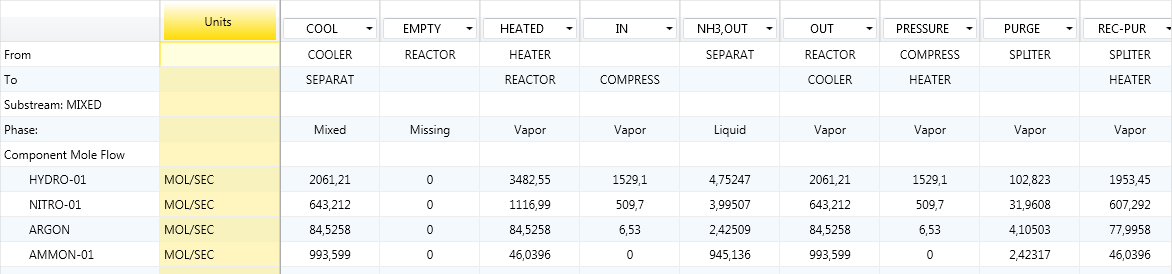
\includegraphics[scale=0.5]{RK-ASPEN.png}
	\end{center}
	\caption{Modèle \texttt{RK-ASPEN}, $750\si{\kelvin}$, $270\si{\bar}$, 5\%}
	\label{fig:RK-ASPEN}
\end{figure}

\begin{figure}[h!]
	\begin{center}
		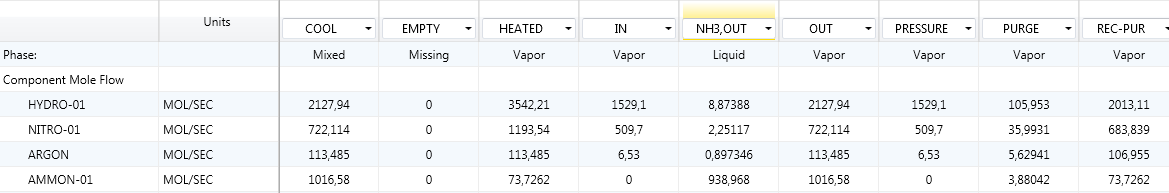
\includegraphics[scale=0.5]{PSRK.png}
	\end{center}
	\caption{Modèle \texttt{PSRK}, $750\si{\kelvin}$, $270\si{\bar}$, 5\%}
	\label{fig:PSRK}
\end{figure}

\begin{figure}[h!]
	\begin{center}
		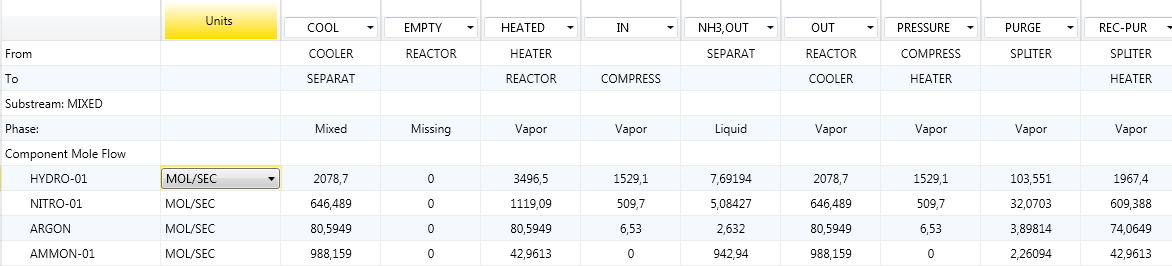
\includegraphics[scale=0.5]{SRK,750,270,5.png}
	\end{center}
	\caption{Modèle \texttt{SRK}, $750\si{\kelvin}$, $270\si{\bar}$, 5\%}
	\label{fig:SRK,750,270,0.05}
\end{figure}

\begin{figure}[h!]
	\begin{center}
		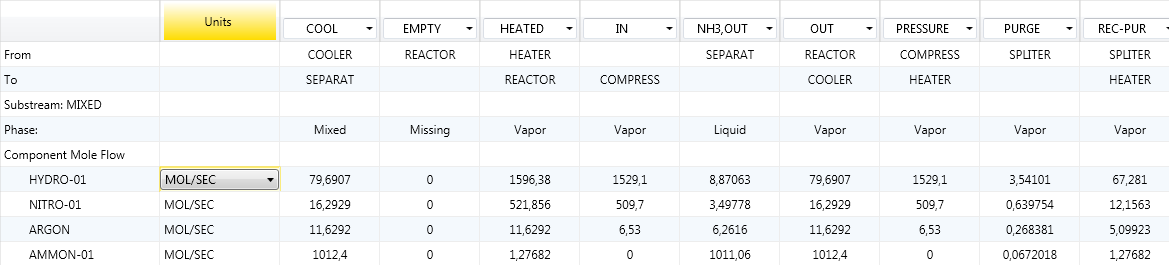
\includegraphics[scale=0.5]{SRK,500,270.png}
	\end{center}
	\caption{Modèle \texttt{SRK}, $500\si{\kelvin}$, $270\si{\bar}$, 5\%}
	\label{fig:SRK,500,270,0.05}
\end{figure}

\begin{figure}[h!]
	\begin{center}
		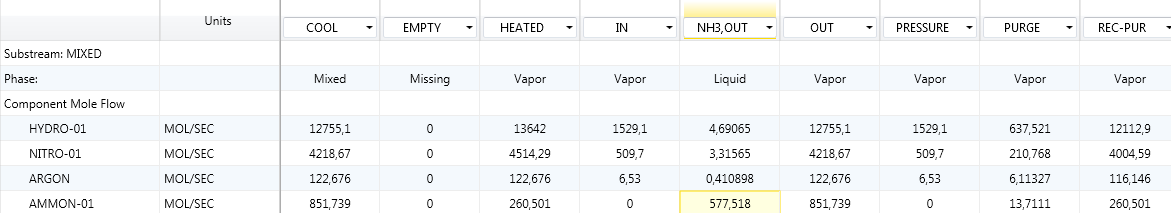
\includegraphics[scale=0.5]{SRK,1000,270.png}
	\end{center}
	\caption{Modèle \texttt{SRK}, $1000\si{\kelvin}$, $270\si{\bar}$, 5\%}
	\label{fig:SRK,1000,270,0.05}
\end{figure}

\begin{figure}[h!]
	\begin{center}
		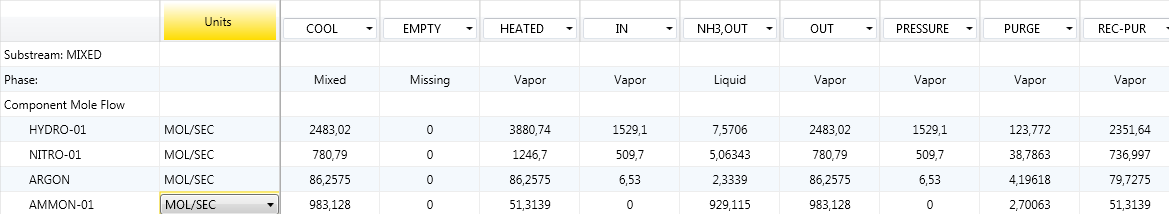
\includegraphics[scale=0.5]{SRK,750,220.png}
	\end{center}
	\caption{Modèle \texttt{SRK}, $750\si{\kelvin}$, $220\si{\bar}$, 5\%}
	\label{fig:SRK,750,220,0.05}
\end{figure}

\begin{figure}[h!]
	\begin{center}
		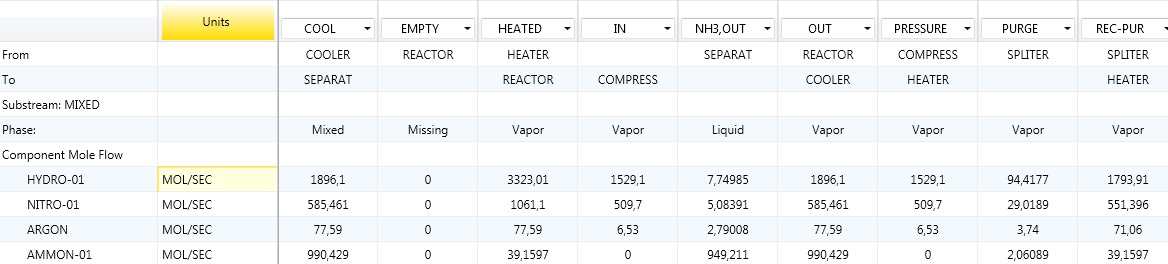
\includegraphics[scale=0.5]{SRK,750,300.png}
	\end{center}
	\caption{Modèle \texttt{SRK}, $750\si{\kelvin}$, $300\si{\bar}$, 5\%}
	\label{fig:SRK,750,300,0.05}
\end{figure}

\begin{figure}[h!]
	\begin{center}
		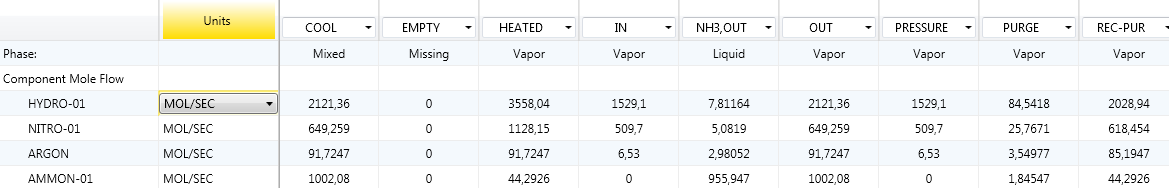
\includegraphics[scale=0.5]{SRK,750,270,4.png}
	\end{center}
	\caption{Modèle \texttt{SRK}, $750\si{\kelvin}$, $270\si{\bar}$, 4\%}
	\label{fig:SRK,750,270,0.04}
\end{figure}

\begin{figure}[h!]
	\begin{center}
		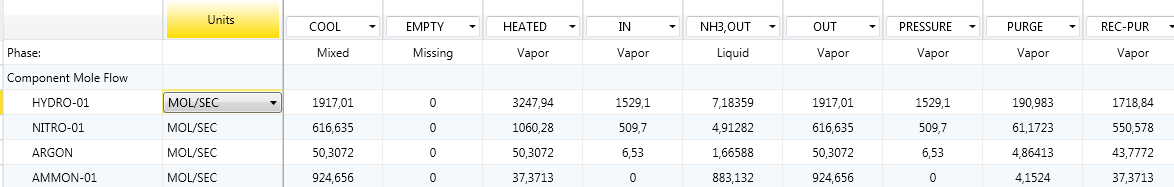
\includegraphics[scale=0.5]{SRK,750,270,10.png}
	\end{center}
	\caption{Modèle \texttt{SRK}, $750\si{\kelvin}$, $270\si{\bar}$, 10\%}
	\label{fig:SRK,750,270,0.1}
\end{figure}

\begin{figure}[h!]
	\begin{center}
		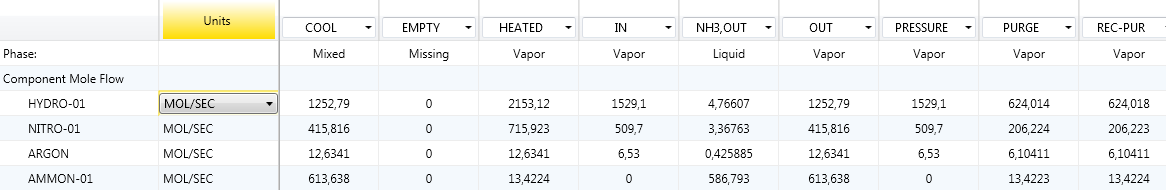
\includegraphics[scale=0.5]{SRK,750,270,50.png}
	\end{center}
	\caption{Modèle \texttt{SRK}, $750\si{\kelvin}$, $270\si{\bar}$, 50\%}
	\label{fig:SRK,750,270,0.5}
\end{figure}

\begin{figure}[h!]
	\begin{center}
		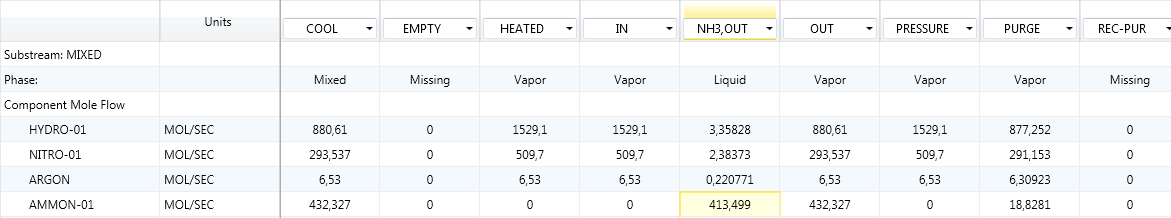
\includegraphics[scale=0.5]{SRK,750,270,100.png}
	\end{center}
	\caption{Modèle \texttt{SRK}, $750\si{\kelvin}$, $270\si{\bar}$, 100\%}
	\label{fig:SRK,750,270,1}
\end{figure}

\section{Outil de calcul: codes \textsc{Matlab}}




\printbibliography
\end{document}



\chapter{T\^ache 4}
%Quels sont les dangers présentés par les substances mises en œuvre durant la synthèse de l’ammoniac ?
\section{Dangers présentés les composés}

On retrouve $6$ gaz présents dans le réacteur. 
Certains ne présentent que peu de danger, 
d'autres peuvent provoquer d'importants dégats en cas de combustion.

\begin{itemize}	
	\item L'hydrogène est un gaz extrêmement inflammable et peut provoquer de grosses 
		explosions en cas de combustion. C'est le principal danger lié à sa présence. 
		En cas d'accumulation d'hydrogène dans une pièce ou un batiment, 
		sa présence peut provoquer un environnement déficient en oxygène et 
		donc provoquer la suffocation.

	\item  L'argon est présent naturellement dans l'air et n'est dangereux qu'en 
		quantités importantes. Il peut alors provoquer la suffocation.

	\item  L'azote est également naturellement présent dans l'air et n'est pas plus 
		dangereux que l'argon.

	\item  L'ammoniac est inflammable et peut donc provoquer une explosion en cas 
		d'accumulation et de combustion.

	\item  L'helium peut provoquer l'asphyxie en cas de concentration trop élevée.

	\item  Le méthane est inflammable et présente un danger d'explosion en cas 
		d'accumulation et de combustion. Il y a également un risque d'asphyxie en 
		cas d'accumulation simple.
\end{itemize}

\section{Circulation des flux de matière}

Les PDF et PID se trouvent à la fin du rapport dans l'annexe \ref{sec:fluxes}.



\section{Étude des dangers et catastrophes potentiels}


\paragraph{1} Imaginons que pour une quelconque raison, il y ait une fuite de gaz inflammable, 
de l'hydrogène par exemple. Le gaz se propagerait alors dans l'atmosphère à 
une pression de $150\si{\bar}$ et à une température de $180\si{\celsius}$. 
Il s'enflammerait directement, créant ainsi une augmentation rapide de la température. 
Les canalisations, chauffées par les flammes, verraient leur pression interne augmenter 
brutalement. Les canalisations se déchireraient, entraînant la libération d'hydrogène 
supplémentaire, provoquant ainsi une déflagration.

Nous pourrions éviter le déchirement des canalisations en utilisant des disques de rupture 
au niveau de celles-ci. Si la pression interne dépasse un certain seuil, le disque de rupture 
se rompt, libérant le gaz, mais évitant la destruction des tuyauteries.

\paragraph{2} Prenons maintenant le cas où un problème survient au niveau du réacteur 
de synthèse de l'ammoniac. La réaction de synthèse

\begin{equation}
	\ce{\frac{3}{2} H2_{(g)} + \frac{1}{2} N2_{(g)} <=> NH3_{(g)}}
	\label{eq:synthesis}
\end{equation}

est une réaction exothermique ($-45.9\si{\kilo\joule}$ à $298\si{\kelvin}$). 
Elle dégage donc beaucoup de chaleur, qu'il faut traiter afin d'éviter 
une hausse trop importante de la température au sein du réacteur. 
En faisant circuler les gaz de synthèse \ce{H2 \, et \, N2},  
qui sont à $180\si{\celsius}$, dans les parois du réacteur, 
ceux-ci vont absorber une partie de la chaleur produite par la réaction. 
Nous nous apercevons donc que s'il y a une défaillance au niveau du système 
de refroidissement, par exemple si l'entrée des gaz de synthèse est bouchée, 
la température du réacteur va augmenter brusquement. Etant donné que le volume est fixe, 
la pression va augmenter proportionnellement à la température, 
jusqu'à ce qu'elle dépasse la limite supportable par les parois du réacteur. 
A ce moment-là, le réacteur explose sous l'effet de la pression.

Pour éviter cela, il faut équiper le réacteur d'une soupape de sécurité, qui permettrait d'évacuer une partie du gaz afin de stabiliser la pression interne du réacteur. 
Nous pouvons également faire en sorte que le couvercle du réacteur cède en premier en cas de surpression, nous limiterions de cette manière fortement les dommages occasionnés.

\paragraph{3} Etudions maintenant le cas d'un blackout électrique. 
L'installation est soudainement privée d'électricité. 
Les compresseurs vont donc s'arrêter, et l'apport en réactifs au niveau 
du réacteur va donc s'arrêter.
La réaction va continuer jusqu'à ce que les pressions au niveau des tuyauteries 
des réactifs et de l'ammoniac s'équilibrent.
La synthèse de l'ammoniac diminue la pression car elle réduit le nombre de moles 
de gaz présent, mais est exothermique, et puisque le refroidissement est effectué 
par les réactifs, et que le système n'est plus alimenté, le réacteur va chauffer.
Il va également falloir redémarrer le réacteur une fois l'élecricité rétablie. 
Le réacteur doit avoir le temps de refroidir afin d'éviter 
que la température ne soit trop élevée lors du redémarrage. 
Il sera cependant nécessaire de purger ou préchauffer le réacteur si
la température du réacteur est trop basse car la réaction ne se fera pas.

Nous pouvons éviter tout problème en ayant des générateurs sur site capable 
de délivrer de l'électricité en cas de blackout jusqu'à ce que 
le courant soit rétablit. 

\section{Soupape de sécurité sur le réacteur de synthèse de l'ammoniac}

% Pourquoi n’y a-t-il pas de soupape de sécurité ou de disque de rupture (les deux types 
% de dispositifs servent à protéger un équipement ou une ligne contre les surpressions) 
% sur le réacteur de synthèse du NH3 ?

Un disque de rupture est un dispositif de sécurité qui sert à protéger les installations 
contre les surpressions.
La réaction de synthèse de l'ammoniac est la réaction \ref{eq:synthesis}.
On remarque immédiatement qu'il y a une diminution du nombre de moles de gaz (d'un facteur 2) 
lorsque de l'ammoniac est produit. La loi des gazs parfait nous indique que la pression
exercée par un gaz est directement proportionnelle à son nombre de moles.
Une surpression n'est pas envisageable pour cette réaction, 
il n'y a donc pas besoin de disque de rupture sur ce réacteur.

\section{Disque de rupture sur l'échangeur \textsc{124-mc}}
% Pourquoi y a-t-il des disques de rupture sur l’échangeur 124-MC ?

L'échangeur 124-C est un dispositif permettant de transférer de la chaleur d'un fluide
vers un autre, sans que ceux-ci ne se mélangent.
On a donc un flux \emph{chaud} et un flux \emph{froid}. Le flux froid va recevoir de 
l'énergie thermique et sa température va augmenter, il faut alors prévoir des disques 
de rupture au cas où la température dépasse une certaine limite qui produirait une 
supression du gaz et pourrait endommager, voire déchirer, la paroi.
Théoriquement, le flux chaud n'a pas besoin de disque de rupture parce que le gaz qu'il 
transporte ne peut que diminuer de volume. Cependant, on peut toujours considérer le cas
d'un apport soudain et imprévu de chaleur comme une explosion extérieure, qui produirait
une augmentation de température et par conséquent de pression. 
Il devient alors nécessaire d'avoir des disques de rupture dans les deux sens de l'échangeur.


\section{Circulation des flux de matières - \textsc{pdf} et \textsc{pid}'s}
\label{sec:fluxes}

\begin{center}
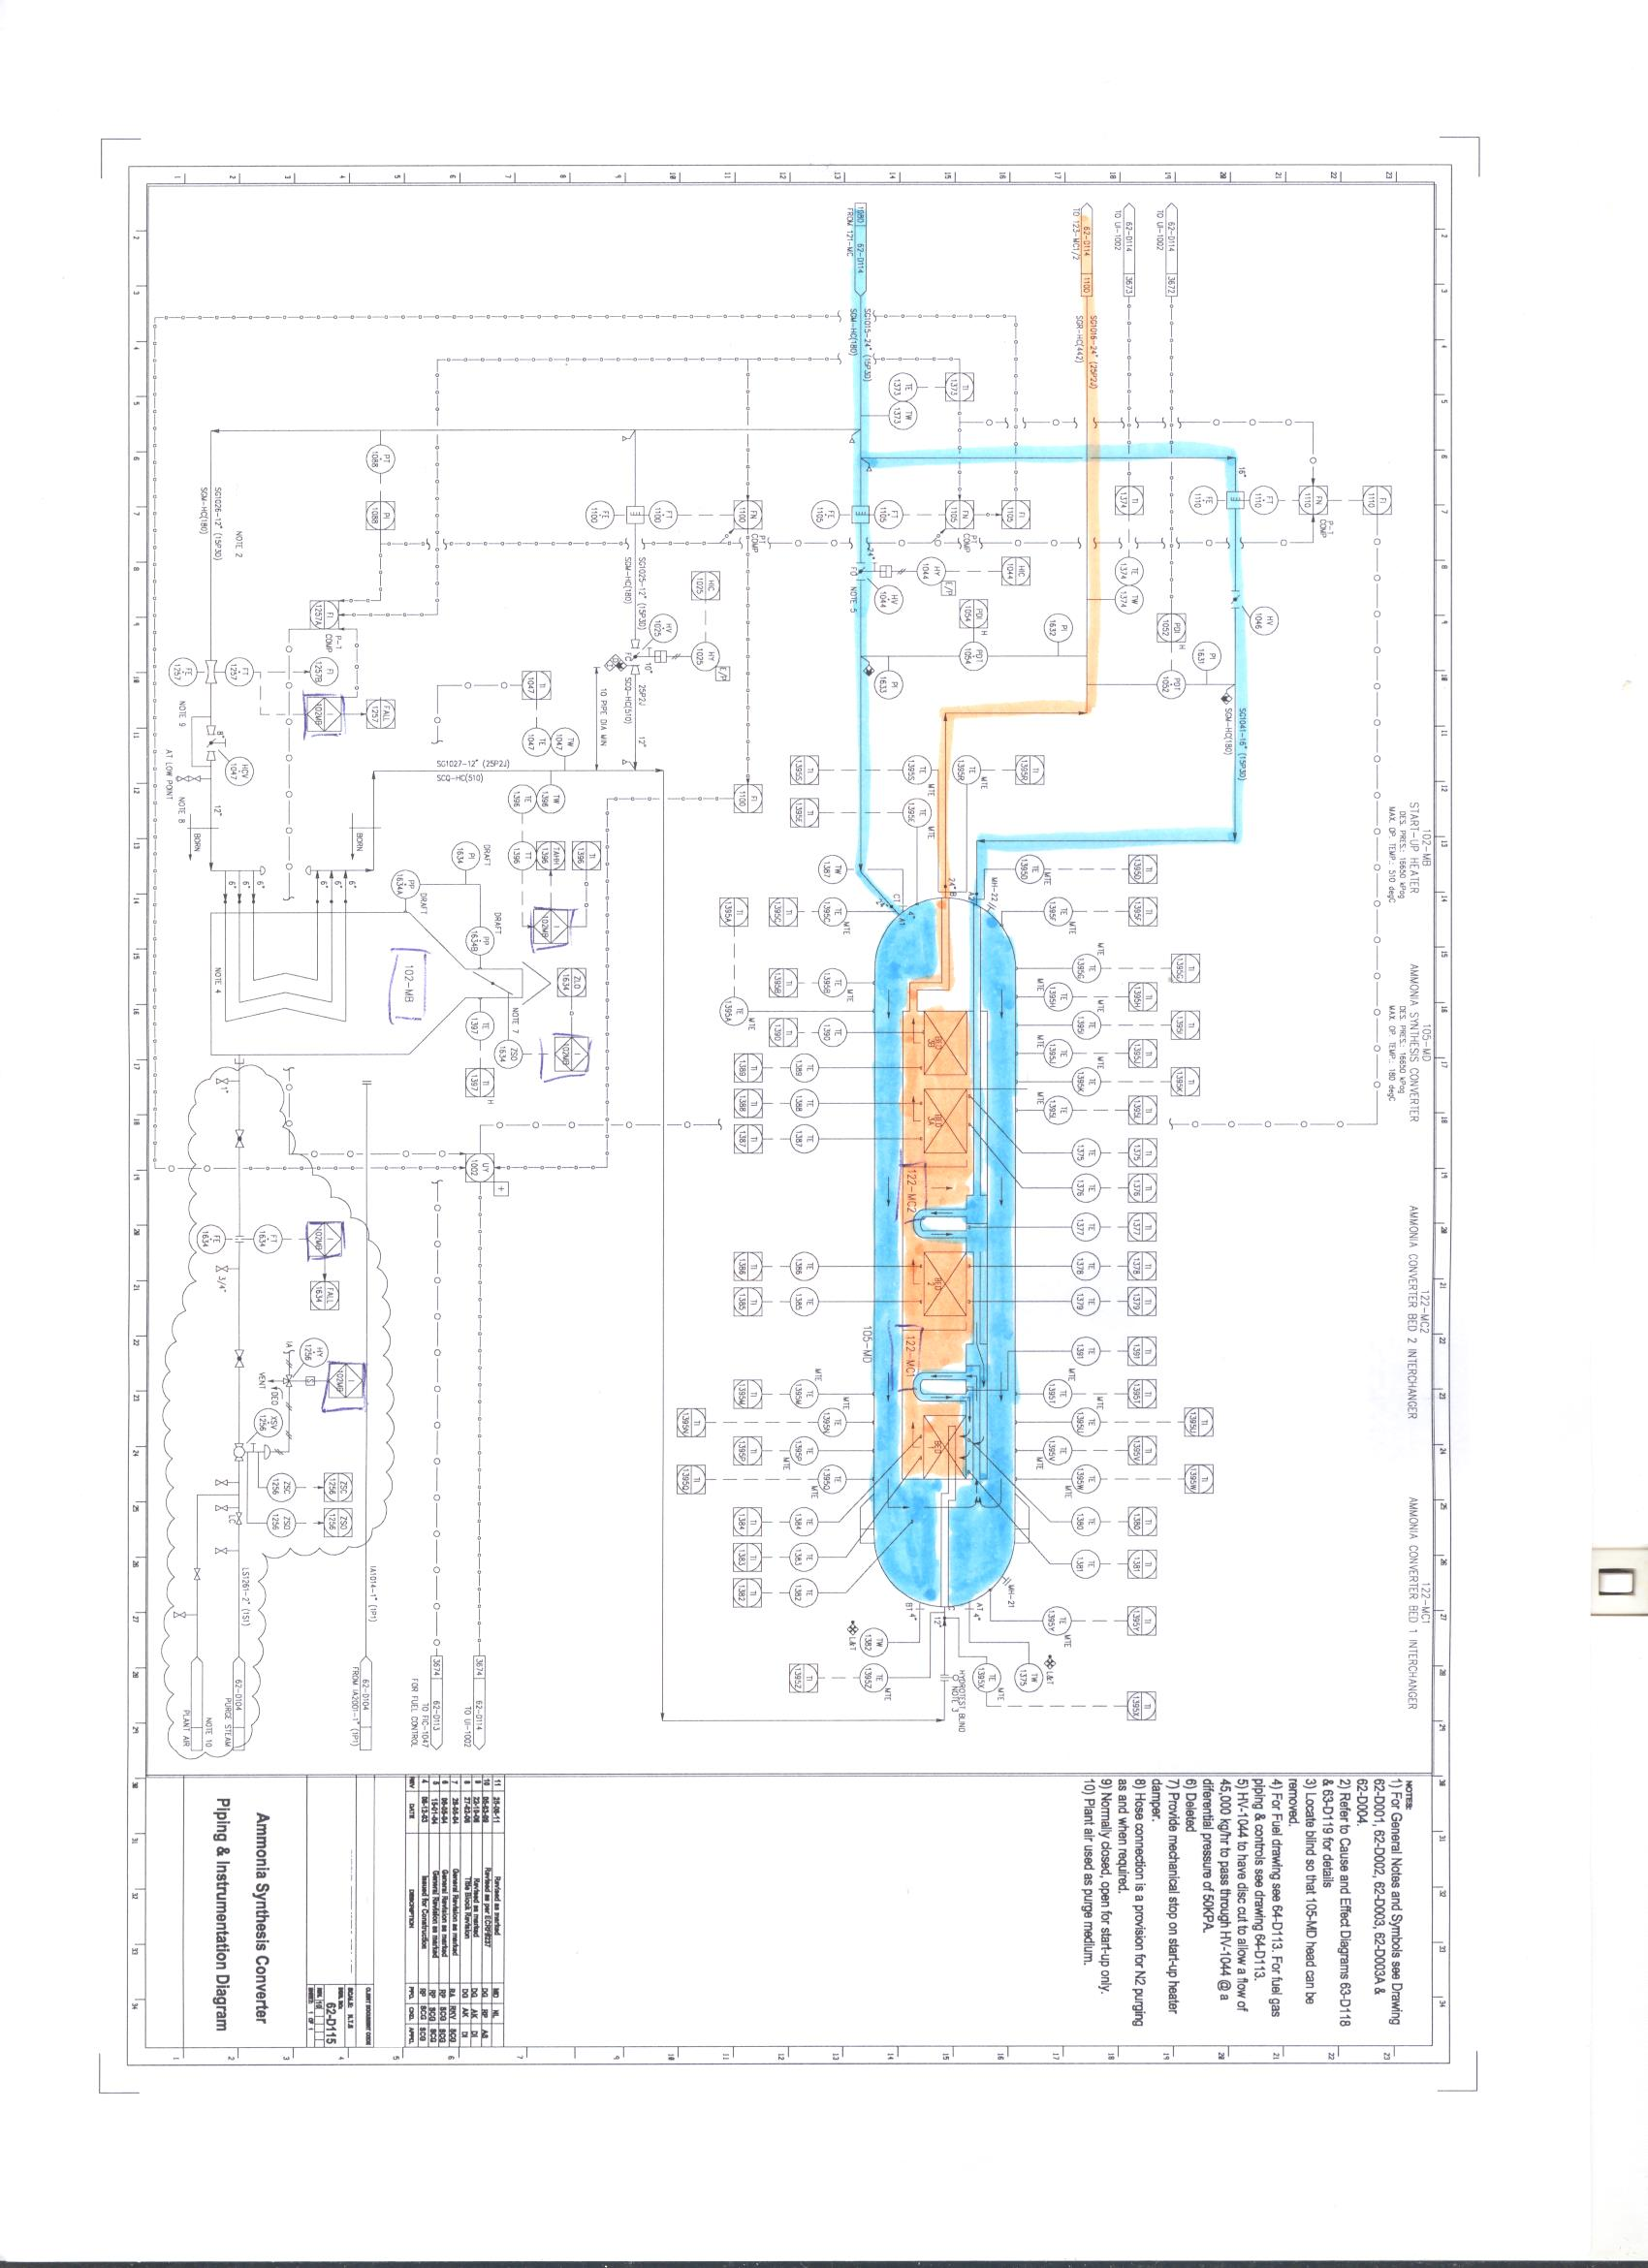
\includegraphics[scale=0.7]{../tache4/img/scan1.jpg}

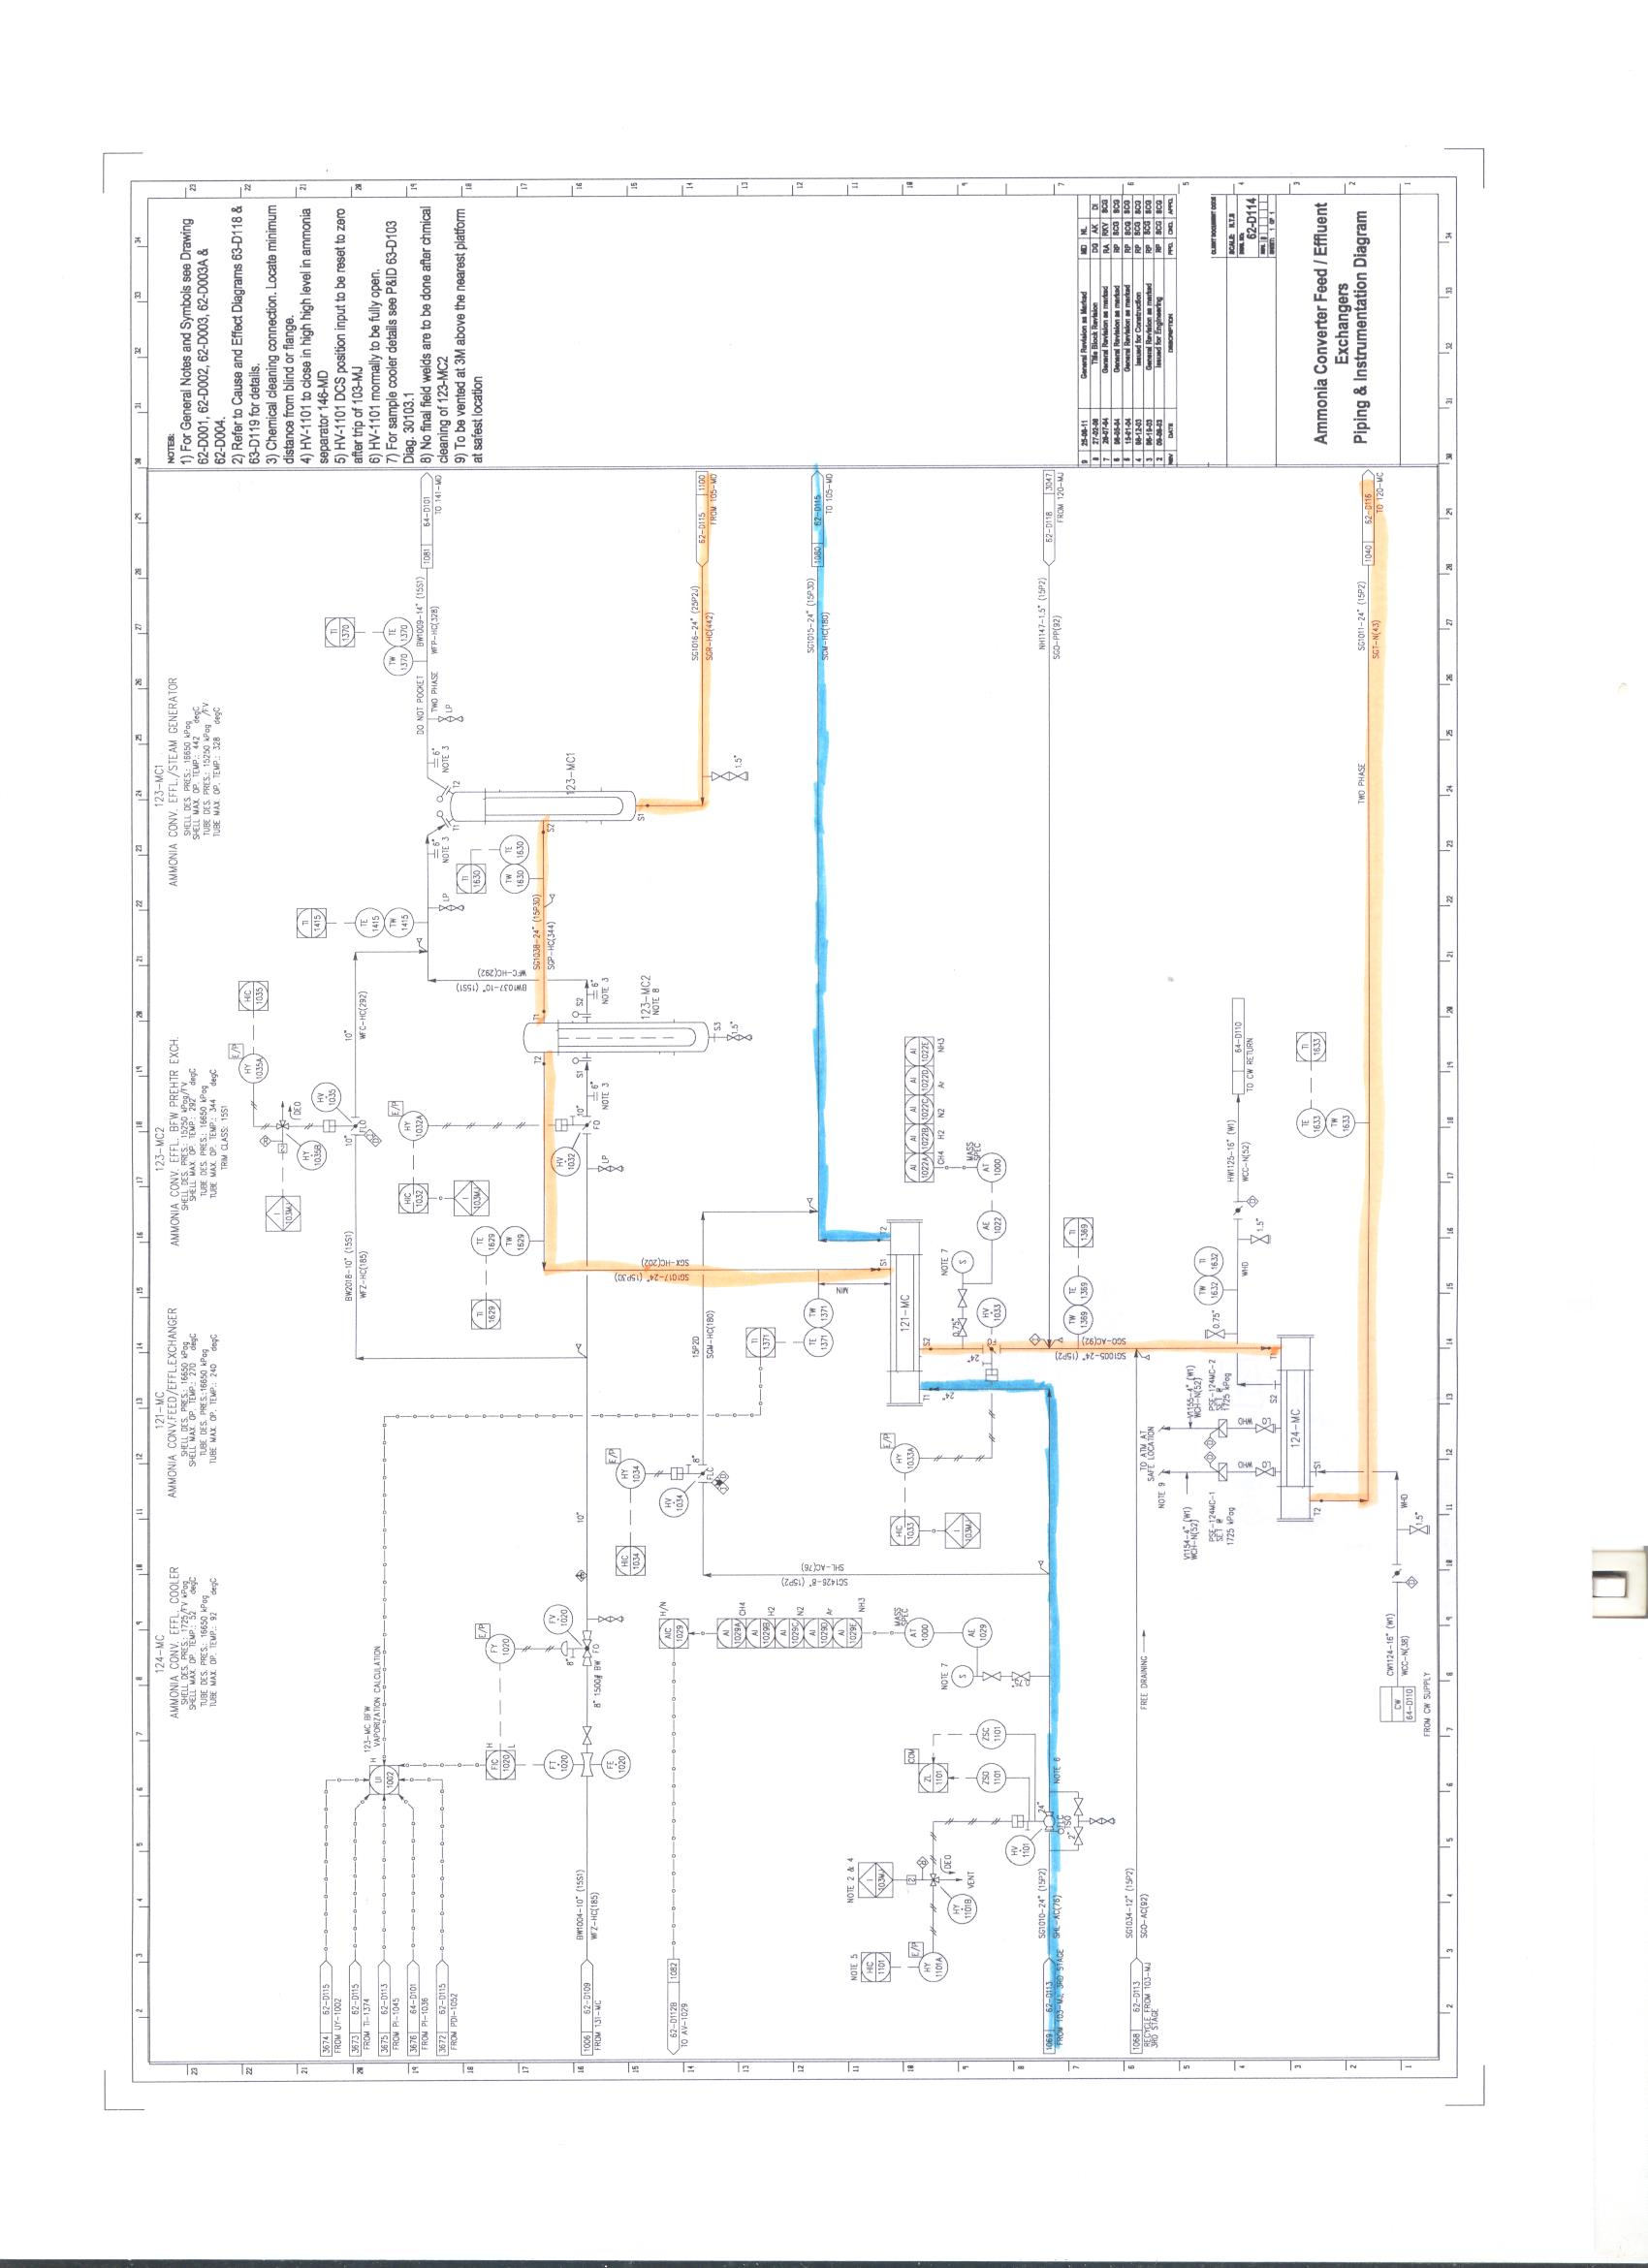
\includegraphics[scale=0.7]{../tache4/img/scan2.jpg}

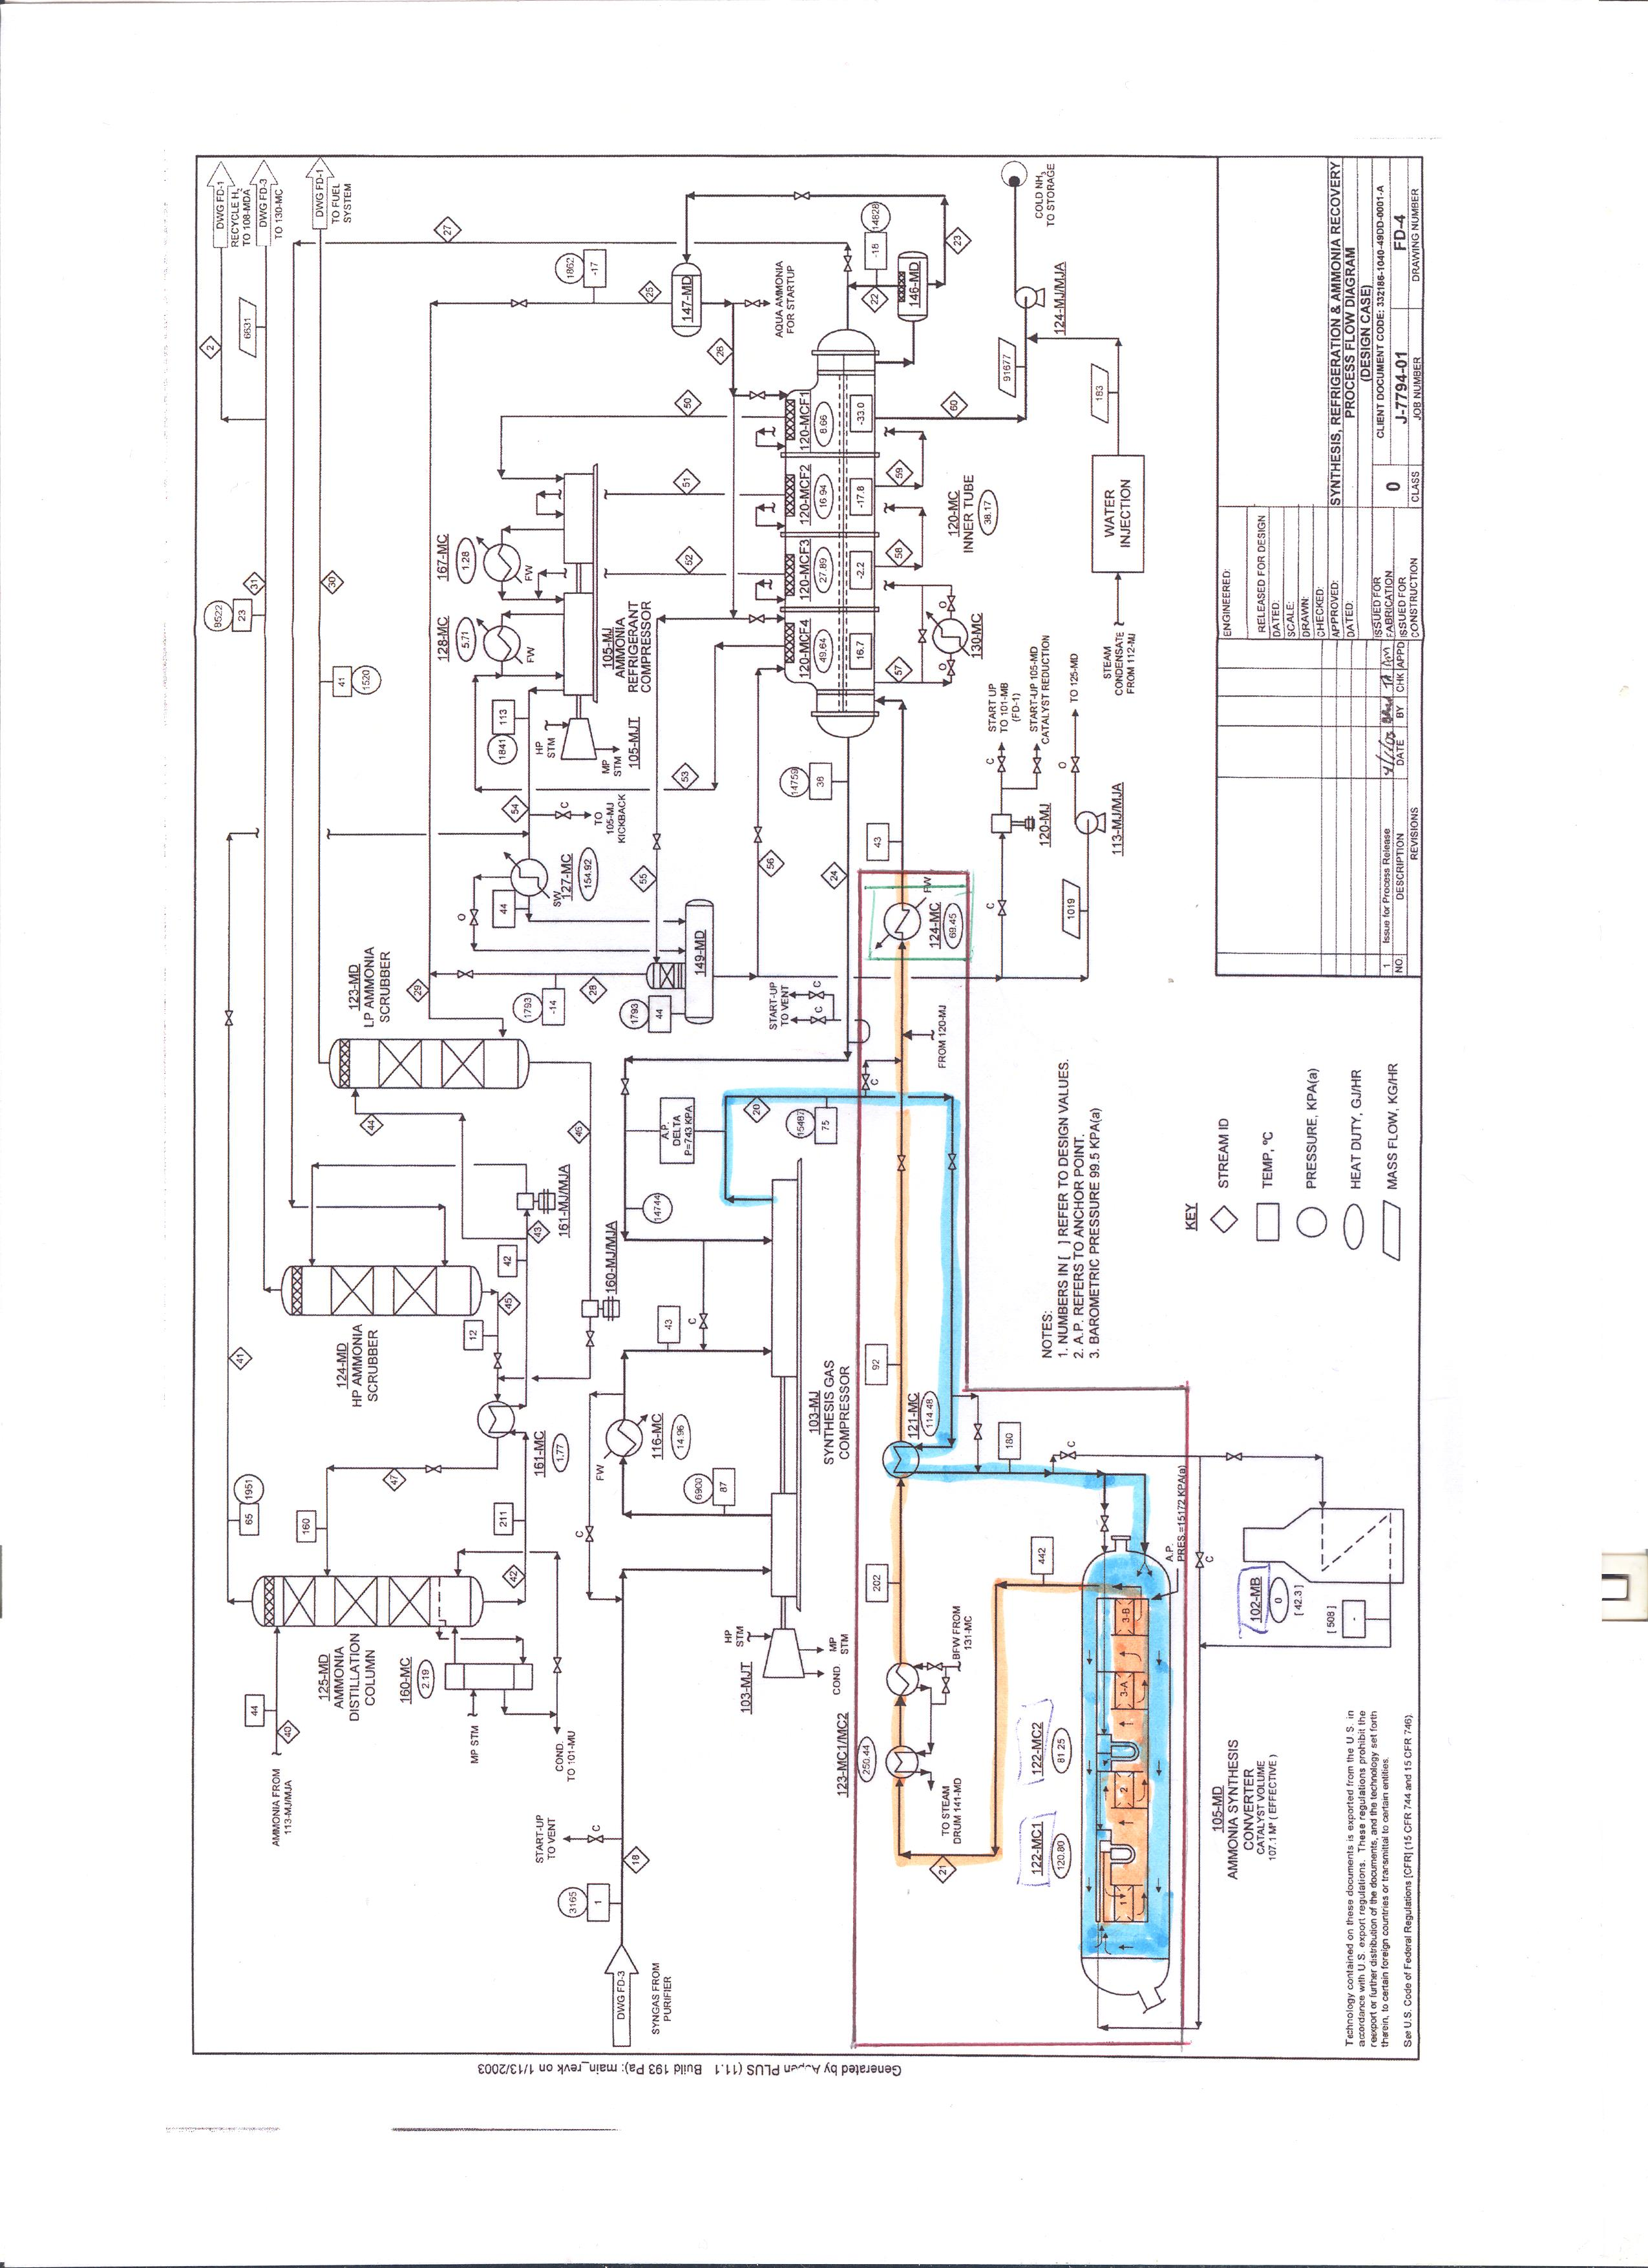
\includegraphics[scale=0.7]{../tache4/img/scan3.jpg}
\end{center}



\chapter{T\^ache 5}
Pour la t\^ache 5, il nous était demandé de dimensionner une soupape de sécurité
pour un tank contenant de l'ammoniac. Pour celà, nous avons recu quelques informations:

\begin{itemize}

\item Forme du tank: cylindrique vertical à extrémités hémisphériques. Tank au sol.
\item Hauteur totale du tank: $12 \si{\metre}$
\item Niveau de \ce{NH3} liquide dans le tank: $8\si{\metre}$
\item Diamètre du tank: $6 \si{\metre}$
\item Température normale de stockage: $20 \si{\degreeCelsius}$
\item Pression de design: $15 \barg$
\item Cp/Cv du \ce{NH3}: $1.33$; Facteur de compressibilité Z: $1.0$
\item La soupape sera une soupape conventionnelle et la contrepression sera nulle.
\item L’usine est munie de systèmes de drainages des fuites 
	et d’un équipement moderne de lutte contre l’incendie.
\end{itemize}

Nous avons également à notre disposition deux graphes donnant respectivement 
les pressions de stockage de l'ammoniac et de l'enthalpie de vaporisation 
en fonction de la température.

\paragraph{Remarque}
A travers cette section nous utilisons l'unité \barg, 
qui correspond à la pression supérieur à la pression atmosphérique.
On a donc:
\[ p [\barg] = p [\si{\bar}] - 1 \]

% Quelle est la pression normale de stockage ?
\section{Pression normale de stockage} 
La pression normale de stockage est de $7.8 \barg$ à $20\si{\celsius}$ 
(température normale de stockage). Nous avons obtenu ces résultats sur base des
graphiques que nous avions reçus.

% Quelle sera la pression de stockage en été (30°C) ?
\section{Pression de stockage en été} 
La pression de stockage en été est de $10.625 \barg$ à $30\si{\celsius}$.

% Quel sera la pression maximale de tarage de la soupape de sécurité ?
\section{Pression maximale de tarage de la soupape} 
La pression maximale de tarage de la soupape de sécurité vaut 
\[ 121\% \cdot p_{\text{design}} = 18.15 \barg \]

% Dimensionner la soupape pour cette pression de tarage.
%     -	Quelle sera la pression durant la décharge ?
%     -	Quelle sera la température du liquide durant la décharge via la soupape ?
%     -	Quelle sera la taille de la soupape nécessaire ?
\section{Dimensionnement de la soupape} 
La pression durant la décharge sera de $19.16325 \si{\bar}$. 
Cette pression est fort élevée car nous considérons le cas d'un incendie au niveau du réservoir. 
La température du gaz durant la décharge sera de $50\si{\celsius}$. 
Nous aurons besoin d'une soupape d'une section de $730\si{\milli\meter\squared}$ 
ou $1.13 \, \text{inch}^2$. Ceci correspond à une PSV de type $2J3$
\[ C = 0.03948 \cdot \sqrt{1.33 \cdot \frac{2}{2.33}^{\frac{2.33}{0.33}}} \]
\[ W = 43200 \cdot 1 \cdot 143.634^{0.82} \]
\[ A = \frac{W}{C \cdot 0.975 \cdot 20.071 \cdot 1 \cdot 1} \cdot \sqrt{\frac{323.15}{17}} \]

\section{Effet de l'augmentation de la pression de tarage de 5 à 20 barg pour une pression de design de 20 barg} 
Si la pression de design est à $20\barg$, nous pouvons augmenter la pression de tarage à \[ 121\% \cdot p_{\text{design}} = 24.2\barg \]

Nous recalculons A avec la pression et température plus élevées,
et obtenons que la soupape doit avoir une section de $590\si{\milli\meter\squared}$
ce qui nous donne $0.9118 \, \text{inch}^2$. Ceci correspond à une PSV de type $2J3$ comme celle trouvée précédemment. Il n'y a donc pas d'intérêt
à augmenter la pression de design dans ces conditions.

% Pour la première pression de tarage, quelle est l’influence d’isoler thermiquement 
% le tank avec un isolant tel que le coefficient d’échange avec l’extérieur 
% soit réduit à une valeur de 10 W/m2.K ? 
\section{Isolation thermique du tank}
Nous isolons la cuve avec un isolant réduisant le coefficient d'échange de la cuve avec l'extérieur à 
$10 \si{\watt}/\si{\meter\squared} \cdot \si{\kelvin}$
On réduit donc le facteur environnemental à $F = 0.15$. 
Notre $W$ va donc être fortement réduit, et nous pouvons donc réduire la taille de la soupape à 
$110\si{\milli\meter\squared}$ ou $0.17 \, \text{inch}^2$. 
Cette PSV est du type $1E2$. L'ajout de l'isolant réduit donc fortement la taille de
la soupape requise.



\chapter{T\^ache 7}
\section{Visite de la station de biométhanisation de l’\textsc{aive} à Tenneville}

L’usine de biométhanisation permet de créer du \ce{CH4} à partir de déchets organiques,
principalement ménagers, mais aussi provenant de parcs à conteneurs, etc.

Premièrement, les déchets sont acheminés par camions au centre de Tenneville.
Avant que les déchets ne soient stockés dans un entrepôt, 
les camions passent à travers un portique afin 
d'y détecter la présence de déchets radioactifs. Ils sont ensuite pesés
puis déchargés dans le premier entrepôt.

Les déchets passent à travers un broyeur et sont acheminés par tapis roulant 
où des aimants permettent d’y retirer les déchets ferreux indésirables.
À cette étape, les déchets sont prêts à entrer dans le digesteur. 
Ce digesteur ressemble à un grand silo d’une capacité de $3000 \si{\meter\cubed}$.
Le principe est assez simple, des bactéries anaérobies vont commencer à digérer 
ces matières organiques en l’absence d’oxygène, ce qui crée du méthane. 
Le méthane sert à la production d’électricité et de chaleur (principe de cogénération).
L’usine est donc autosuffisante en termes d'électricité et de chauffage.
Le surplus  d’électricité est redistribué sur le réseau, et l’excédent de chaleur 
est utilisé pour le séchage de boue ainsi que dans d’autres usines de recyclage. 

Une fois la matière digérée, elle est compostée complètement jusqu’à l’obtention 
de terreau qui est revendu aux agriculteurs.
En cas de panne de moteur - ou tout autre problème dans le digesteur -
il y a une torchère qui permet du brûler tout surplus de méthane
et donc d'éviter tout excès dans le digesteur. Cela évite aussi de devoir 
libérer du méthane dans l’atmosphère.

Quelques chiffres :
\begin{itemize}
	\item Capacité de traitement : $39 000$ tonnes par an
	\item Production en électricité : équivalent à la consommation de $1500$ ménages
	\item Production de gaz : $55\%$ de \ce{CH4}, $44\%$ de \ce{CO2} + autres gaz
\end{itemize}

\section{Visite du centre Total Research Technology Feluy}

\subsection{Catalyse}
\label{subsec:catalyse}

L'utilisation d'un catalyseur est essentielle pour de nombreuses réactions industrielles 
effectuées aujourd'hui. De nombreuses réactions ne seraient même pas possibles sans 
l'utilisation d'un catalyseur.
 
Un catalyseur réduit l'énergie d'activation d'une réaction en affaiblissant les liens
électroniques des molécules devant réagir, ou en affaiblissant les liens entre les 
molécules des réactifs. Certains catalyseurs sont en pratique ``consommés'' durant 
la réaction (ex: emprisonnés dans les molécules) et d'autres ne sont simplement pas 
affectés par les réactions. 

Dans de nombreuses réactions, les catalyseurs ont également d'autres rôles. 
Suivant le catalyseur utilisé, certaines réactions seront favorisées au détriment 
d'autres (il faut donc trouver un catalyseur favorisant la réaction voulue). 
Le catalyseur peut également déterminer la structure des molécules obtenues lors 
d'une cristallisation. Suivant le catalyseur utilisé lors de la synthèse de polyéthylène,
on obtiendra une poudre fine ou de plus gros grains,
deux structures ayant des applications différentes.
 
Trouver le bon catalyseur est donc essentiel dans la chimie moderne.
 
\subsection{Unités Pilotes}
 
Le développement de nouveaux procédés ou catalyseurs commence tout d'abord en laboratoire,
ou de microréacteurs permettent de tester la viabilité des nouveaux développements.
Si un catalyseur ou un procédé est considéré comme intéressant,
il va ensuite être testé dans une unité pilote. 

Différentes réactions demandent différents réacteurs,
et le réacteur idéal pour une nouvelle réaction est déterminé en laboratoire.
 
Les unités pilotes sont des réacteurs industriels réduits utilisés pour tester de
nouvelles réactions ou de nouveaux procédés. Les unités pilotes sont beaucoup plus
modulables que les unités industrielles. Celles-ci vont permettre de détecter
d'éventuels problèmes qui sont passés inaperçus lors des tests en laboratoires,
ainsi que de déterminer les conditions idéales pour l'utilisation des nouvelles réactions.
Si un nouveau produit (nouvelle structure ou autre) est considéré comme intéressant,
les unités pilotes vont permettre de produire une quantité limitée de ce nouveau
produit afin de fournir des échantillons à des partenaires commerciaux.
Elles évitent ainsi de devoir reconfigurer des plants de grande taille.

\section{Laboratoire d’électrolyse}

L'électrolyse de l'eau est un procédé qui permet de décomposer 
celle-ci en dioxygène et en dihydroègne, tous deux à l'état gazeux.

\begin{equation*}
	\ce{H2O_{(g)} <=> \frac{1}{2} \, O2_{(g)} + H2_{(g)}} 
\end{equation*}

Afin de produire du dihydrogène gazeux en quantités décentes, l'électrolyse de l'eau 
demande énormément d'énergie électrique (sous forme de courant). De plus, le rendement
de la réaction d'électrolyse de l'eau ne dépasse en général jamais les $50\%$.

Sur base des expérimentations effectuées en laboratoire, nous observons que pour un même volume de dihydrogène produit, 
plus l’intensité du courant est élevée, plus le temps nécessaire à la production
du dihydrogène est faible. En fait, le courant et le temps sont inversément proportionnels, 
et nous pouvons écrire la relation suivante :

\begin{equation*}
	It = \text{constante}
\end{equation*}

où I est l'intensité du courant électrique, et t, le temps écoulé. 
Cela montre bien que lorsqu'on augmente le courant, le temps diminue dans les mêmes proportions.

Calculons maintenant la puissance nécessaire pour produire tout l'hydrogène 
dont nous avons besoin pour un débit d'ammonicac de 1500 t/j.

En prenant une température de $1000 \si{\kelvin}$ pour le reformeur primaire, 
nous savons grâce à notre outil de calcul que pour produire 1500 t/j d'ammoniac, il faut $266,32 \si{\tonne}$ de dihydrogène 
par jour. Cela nous donne un débit massique de $184,944 \, \si{\kilo\gram/\minute}$.

Nous devons maintenant fixer trois paramètres pour le déroulement de la réaction d'électrolyse : le pH, la température et le courant.
La réaction d'électrolyse nécessite une puissance moins importante lorsque le pH tend vers 0. Mais un pH nul demande une grande quantité d'acide, nous allons donc nous contenter ici d'un pH = 1.
Par souci d'économie d'énergie, nous allons travailler à température ambiante, soit $20\si{\celsius}$.
Le dernier paramètre est le courant, que nous allons faire varier afin d'obtenir la quantité voulue d'hydrogène.
Par exemple, en appliquant un courant de $0,5 \si{\ampere}$, nous savons, grâce aux expériences faites en laboratoire, 
que nous produisons $4 \, \si{\milli\liter}$ de dihydrogène par minute. 
Considérons maintenant que le dihydrogène se comporte comme un gaz parfait, nous pouvons appliquer :

\begin{equation*}
	pV = mR^{*}T
\end{equation*}

et donc calculer la masse de dihydrogène, sachant que la réaction se déroule 
sous une température de $293,15 \si{\kelvin}$ et une pression de $1 \si{\bar}$. 
Nous obtenons ainsi qu'en faisant circuler un courant de $0.5 \si{\ampere}$, 
nous produisons $3,2824\e{-7} \, \si{\kilo\gram/\minute}$ de dihydrogène.

Pour atteindre un débit massique de $184,944 \, \si{\kilo\gram/\minute}$, 
il faut donc un courant électrique de $2,817\e{8} \si{\ampere}$. 
Nous savons grâce aux résultats du laboratoire que la tension électrique dépend quant à elle du pH. 
Pour un pH = 1, la tension appliquée par la source sera de 10 V.
Nous pouvons alors calculer la puissance électrique grâce à la relation suivante : 

\begin{equation*}
	P = UI
\end{equation*}

La puissance est donc égale à $2,817 \, \si{\giga\watt}$.

Cette puissance requise est énorme. L'électrolyse de l'eau demande 
beaucoup trop de puissance pour produire ce dont nous avons besoin. 
C'est pour cela que l'électrolyse est encore très peu utilisée à l'échelle industrielle. 
Il est donc préférable dans notre cas de se contenter du vaporeformage, 
malgré le fait qu'il émette du dioxyde de carbone.

\section{Visite du plant de Yara à Tertre}

Le plant de Yara fabrique des engrais et produit lui-même son propre ammoniac nécessaire
pour créer ces engrais. Avoir une production locale d'ammoniac permet non seulement 
d'éviter des coûts importants mais aussi d'éviter le transport de celui-ci car il 
peut s'avérer être toxique.

Tout d'abord, le réacteur où est synthétisé l'ammoniac est à une pression de $130 \si{\bar}$.
Comme décrit dans la section \ref{subsec:catalyse}, l'utilisation de catalyseurs dans la
production du méthane est fondamentale. Un catalyseur est utilisé lorsque la 
barrière énergétique pour qu'une réaction se produise est trop haute. Il va alors 
diminuer l'énergie d'activation sans modifier le chemin réactionnel.

Le diagramme de la figure \ref{fig:synthese} présente le fonctionnement simplifié 
des réacteurs de synthèse d'ammoniac. Il est important de préciser que le \emph{input}
est tout d'abord composé d'hydrogène et d'azote mais aussi de résidus de méthane, 
d'argon et d'hélium. Ceux-ci sont éliminés via différentes techniques 
de séparation (ex: par des membranes semi-perméables). 

\begin{figure}[h!]
	\begin{center}
		\begin{tikzpicture}
[node distance = 7em]

\tikzstyle{block} = [rectangle, draw, fill=blue!20, 
    text width=10em, text centered, rounded corners, minimum height=3em]
\tikzstyle{block2} = [rectangle, draw, fill=red!60, 
    text width=6em, text centered, minimum height=2em]
\tikzstyle{line} = [draw, -latex']
\tikzstyle{cloud} = [draw, ellipse,fill=red!20, node distance=2cm,
    minimum height=1em]
    
\node [block2] (purge) {Purge};
\node [block, below = 4em of purge] (compresseur) {Compresseur/Synthèse};
\node [cloud, right = 10em of purge] (input) {Input};
\node [block, right = 6em of compresseur] (cooler) {Refroidisseur};
\node [block, below = 4em of cooler] (separation) {Separation};
\node [cloud, left = 8em of separation] (output) {Output};

\path [line] (input) -- node[anchor = south] {\ce{N2} \ce{H2} \ce{CH4} \ce{Ar} \ce{He}}
	(purge);
\path [line] (purge) -- node[anchor = west] {\ce{N2} \ce{H2}}
	(compresseur);
\path [line,dashed] (compresseur) -- node[anchor = south] {\ce{NH3_{(g)}} \ce{NH3_{(l)}}} 
	(cooler);
\path [line,dashed] (cooler) -- node[anchor = west] {\ce{NH3_{(g)}} \ce{NH3_{(l)}}} 
	(separation);
\path [line,dashed] (separation) -- node[anchor = east] {\ce{NH3_{(g)}}}
	(compresseur);
\path [line] (separation) -- node[anchor = north] {\ce{NH3_{(l)}}} 
	(output);
\end{tikzpicture}


	\end{center}
	\caption{Fonctionnement simplifié de la synthèse d'ammoniac.}
	\label{fig:synthese}
\end{figure}

Une autre information importante concerne la quantité d'énergie nécessaire pour produire
une tonne d'ammoniac. Théoriquement on devrait avoir besoin de $20 \si{\giga\joule/\tonne}$
pour l'ensemble du processus. On observe cependant qu'il nous faut 
pratiquement $30 \si{\giga\joule/\tonne}$. On remarque donc qu'une partie 
importante de l'énergie est perdue à travers les différentes transformations. 
Ces pertes peuvent provenir par exemple d'une qualité non optimale (d'un point de vue 
de rendement) des réacteurs ou de tuyauteries peu isolantes thermiquement.

Le dernier point essentiel de la visite concerne la partie sur l'impact environnemental 
de la société. On compte environ $1000$ tonnes par jour de \ce{CO2} produit, une moitié,
dite impure, sera rejetée dans l'atmosphère tandis que l'autre moitié, dite pure, 
sera reliquéfiée pour ensuite être revendue (utile pour la production de bière par exemple).
On notera aussi le rejet de composés très polluants tels que le \ce{NO2} et le \ce{NOx} 
qui proviennent des fumées du reformage primaire à cause d'un manque d'efficacité
du brûleur.

\section{Atelier créatif (conduite de brainstorming)}

Comment faire preuve d'inventivité et d'originalité dans un projet tel que le nôtre ?
Tel était le thème de cet atelier où l'on nous a présenté le cheminement 
à suivre afin de mettre un maximum à profit la créativité de chacun.

Dans notre cas, la créativité est avant tout l'art de trouver des solutions 
originales et efficaces à un problème bien posé. 
La première partie du travail consiste donc à reformuler la problématique de façon 
à être capable de diverger et de trouver un angle nouveau sous lequel analyser le problème. 
Pour cela, il est conseillé de faire un schéma sur lequel on pourra retrouver différents
éléments comme par exemple les services attendus, la position géographique, 
ce qui se situe à proximité de l’usine,etc.

Cette représentation permet d'avoir une vue d'ensemble sur le travail qui 
devra être effectué et facilite donc l'organisation. Il est important de pousser tout
le monde à sortir de sa ``zone de confort'' et de confronter les idées de chacun.
Vient ensuite le retour à la réalité: il faut analyser les idées, choisir celles qui 
sont réalisables pour que le projet se précise enfin. De nombreux exercices ont été 
proposés afin de nous mettre en situation. 

Nous pouvons à présent faire bénéficier le reste du groupe de notre expérience et tenter
de suivre cette approche. Il est nécessaire de faire un résumé de tout cela pour essayer 
de convaincre et de prouver la viabilité de l'ébauche. Pour cela, on fait la liste 
de quatre choses: les besoins du client, la promesse, les raisons d'y croire, 
et un slogan pour accrocher. On continue l'argumentation avec des analogies,
des choses factuelles (brevets,...) ou inspirantes, etc. Le projet pourra alors
enfin être mis en place!

Une présentation sur le développement durable a aussi été faite afin de nous sensibiliser
et nous inviter à essayer d'y participer. 
En effet, notre système industriel actuel - où la recherche du profit occupe une position
centrale - est voué à l'échec, car il mène à des crises dans de nombreux domaines.
C'est pourquoi la société doit se remettre en question et évoluer pour atteindre
l'idéal d'un système organique, où l'humanité travaillerait ensemble pour un but commun. 

Dans notre cas, cela se résume à se préoccuper de l'écologie mais pas uniquement:
il serait intéressant de collaborer avec d'autres sociétés au niveau de l'importation
des ressources et de l'exportation nos déchets. Ces derniers pourraient être utiles
à d'autres et nous pourrions ainsi trouver des ententes profitables pour tous,
s'approchant d'un système cyclique.

%\documentclass[12pt,oneside]{article}

\NeedsTeXFormat{LaTeX2e}
\ProvidesPackage{custom}[2014/05/11 Custom Package]

\usepackage[utf8]{inputenc}
\usepackage[T1]{fontenc}
\usepackage[francais]{babel}

\usepackage[version=3]{mhchem}
\usepackage{chemfig}

\usepackage{amsmath}
\usepackage{amsthm}
\usepackage{amsfonts}

\usepackage{graphicx} 
\usepackage[top=3cm, bottom=3cm, left=3cm , right=3cm]{geometry}
%\usepackage{setspace} %doublespace, onehalfspace
\usepackage{siunitx}

\usepackage{tikz}
\usetikzlibrary{positioning}
\usetikzlibrary{shapes,arrows}

\usepackage{tabularx}
\usepackage{url} 
\usepackage{tocloft} %spacing in list of figures
\usepackage{listings} %input code
%\usepackage{multibbl} %multiplebibliography
\usepackage{hyperref}
\usepackage[babel=true]{csquotes}
\usepackage{listings}
\usepackage{color}

\usepackage{epstopdf}

\usepackage{caption}
\usepackage{subcaption}
\usepackage{float}

\newcommand{\dif}[1]{\mathrm{d}#1}
\newcommand{\e}[1]{\cdot 10^{#1}}

\endinput


\title{Annexe 3 - Préparation du laboratoire d'électrolyse}
\author{Groupe 1225}
\date{Lundi 3 Novembre}

\begin{document}

\maketitle

Les valeurs exactes demandées ainsi que le graphique de l'évolution de l'équilibre
dans la solution en acide sulfurique en fonction du pH sont obtenus en
exécutant la fonction \texttt{electrolyse.m}.

\section{Solution à pH acide}

Nous devons déterminer le volume (en \si{\milli\liter}) de \ce{H2SO4} (5M)
nécessaire pour atteindre un certain pH.
Il s'agit donc de prendre en compte le fait qu'une fois que tout 
le \ce{H2SO4} sera transformé en \ce{HSO4-}, celui-ci à son tour contribuera
à l'augmentation du pH étant donné que c'est un acide faible.

Les deux réactions sont les suivantes

\begin{align*}
	\ce{H2SO4 + H2O <-> HSO4- + H3O+} \\
	\ce{HSO4- + H2O <-> SO4^{2-} + H3O+}
\end{align*}

On connait le pH de la solution, $K_{a1}$\footnote{On observe que malgré le fait 
que $K_{a1}$ soit très grand, la réaction n'est pas totalement complète et il est
donc important de calculer l'équilibre pour la première fonction de \ce{H2SO4}.}
et $K_{a2}$ qui sont les constantes d'équilibre associées respectivement 
à la première et la seconde réaction.

On obtient donc un système de trois équations où les trois inconnues
sont $x$ le nombre de moles initial de \ce{H2SO4}, $\xi_1$ et $\xi_2$
les degrés d'avancement des réactions.

\begin{align*}
	K_{a1} &= \frac{\xi_1^2}{x - \xi_1} \\
	K_{a2} &= \frac{\xi_2 \, (\xi_1 + \xi_2)}{\xi_1 - \xi_2} \\
	\text{pH} &= - \log_{10}{(\xi_1 + \xi_2)} 
\end{align*}

Ce système est résolu dans \texttt{electrolyse.m}.

\section{Solution à pH basique}

Nous devons à nouveau déterminer le volume (en \si{\milli\liter}) 
de \ce{NaOH} (5M) nécessaire pour atteindre un certain pH.
Cette partie est beaucoup plus simple étant donné que l'hydroxide de sodium
est une base forte et n'a qu'une seule fonction basique.

Par la relation suivante

\[
	[\ce{OH-}] \cdot [\ce{H3O+}] = 10^{-14} 
\]
On trouve très facilement que 

\[
	V_{\ce{NaOH}} = \frac{10^{-14}}{10^{- \text{pH}}} \cdot 200 
	\quad \text{(en \si{\milli\liter})}
\]



\end{document}



>>>>>>> FETCH_HEAD

\printbibliography
\end{document}

